\documentclass[12pt, %
openright,
oneside, %
%twoside, %TCC: Se seu texto tem mais de 100 páginas, descomente esta linha e comente a anterior
a4paper,    %
english,   % necessário para o Abstract
brazil]{facom-ufu-abntex2}

\usepackage{graphicx}
\graphicspath{{figuras/}{pictures/}{images/}{./}} % where to search for the images

%, Pacotes adicionais para este trabalho, 
\usepackage{amsmath}    % ambientes e comandos matemáticos
\usepackage{amssymb}    % símbolos matemáticos
\usepackage{float}      % posicionamento [H] de figuras/tabelas
\usepackage{array}      % colunas customizadas (>{...})
\usepackage{booktabs}   % \toprule \midrule \bottomrule
\usepackage{tabularx}   % tabelas que ajustam largura ao texto

\newcommand{\blue}[1]{\textcolor{blue}{#1}}
\newcommand{\red}[1]{\textcolor{red}{#1}}

%, Fonte (origem) padronizada de figuras e tabelas (padrão ABNT), 
% (\fonte já é definido pela classe abntex2; usamos um nome próprio)
\newcommand{\fontefig}[1]{%
  \par\nopagebreak\vspace{0.15cm}%
  {\centering\footnotesize Fonte: #1\par}%
}

%, 
% Dados da CAPA, FOLHA DE ROSTO e identificação do curso
% (sobrescrevem os padrões da classe FACOM para o curso de Gestão da Informação)
%, 
\instituicao{%
  Universidade Federal de Uberlândia -- UFU
  \par
  Faculdade de Gestão e Negócios -- FAGEN
  \par
  Bacharelado em Gestão da Informação}

\tipotrabalho{Trabalho de Conclusão de Curso}

\preambulo{Trabalho de Conclusão de Curso apresentado à Faculdade de Gestão e
Negócios da Universidade Federal de Uberlândia, como parte dos requisitos
exigidos para a obtenção do título de Bacharel em Gestão da Informação.}

\local{Uberlândia}

\autor{Marcos Rodrigues de Oliveira Júnior}
\data{2026}
\orientador{Prof. Dr. José Eduardo Ferreira Lopes}
%\coorientador{Algum?}

\titulo{Auditoria de Sistemas de Inteligência Artificial em Plataformas de
Streaming: um Estudo Experimental sobre Vieses e Recomendação Musical no Spotify}

\hypersetup{pdfkeywords={Auditoria algorítmica}{Sistemas de recomendação}{Spotify}{Diversidade musical}{Viés de popularidade}}

\begin{document}
\frenchspacing

% ----------------------------------------------------------
% ELEMENTOS PRÉ-TEXTUAIS
% ----------------------------------------------------------
\imprimircapa
\imprimirfolhaderosto

%, 
% Folha de aprovação (preencher após a defesa; ou descomentar a linha abaixo
% para incluir o PDF escaneado da folha assinada)
%, 
% \includepdf{folhadeaprovacao_final.pdf}
\begin{folhadeaprovacao}

  \begin{center}
    {\ABNTEXchapterfont\large\imprimirautor}

    \vspace*{\fill}\vspace*{\fill}
    {\ABNTEXchapterfont\bfseries\Large\imprimirtitulo}
    \vspace*{\fill}

    \hspace{.45\textwidth}
    \begin{minipage}{.5\textwidth}
        \imprimirpreambulo
    \end{minipage}%
    \vspace*{\fill}
   \end{center}

   Trabalho aprovado. \imprimirlocal, \rule[-0.2em]{2.5em}{0.4pt} de
   \rule[-0.2em]{7em}{0.4pt} de 2026:

   \assinatura{\textbf{\imprimirorientador} \\ Orientador}
   \assinatura{\textbf{Professor(a)} \\ Avaliador(a) 1}
   \assinatura{\textbf{Professor(a)} \\ Avaliador(a) 2}

   \begin{center}
    \vspace*{0.5cm}
    {\large\imprimirlocal}
    \par
    {\large\imprimirdata}
    \vspace*{1cm}
  \end{center}

\end{folhadeaprovacao}
%, 

% As seções dedicatória, agradecimento e epígrafe são opcionais.
% Descomente e preencha caso julgue pertinente.
%\begin{dedicatoria}
%   \vspace*{\fill}\centering\noindent
%   \textit{Dedico este trabalho a \ldots}
%   \vspace*{\fill}
%\end{dedicatoria}
%
%\begin{agradecimentos}
%Agradeço a \ldots
%\end{agradecimentos}
%
%\begin{epigrafe}
%    \vspace*{\fill}
%	\begin{flushright}\textit{``Citação \ldots''}\end{flushright}
%\end{epigrafe}

%, 
% RESUMO em português
%, 
\begin{resumo}
Os sistemas de recomendação algorítmica consolidaram-se como principais
mediadores entre a obra musical e o ouvinte, operando como caixas-pretas cujos
critérios de seleção permanecem opacos. Este trabalho audita o sistema de
recomendação do Spotify sob a ótica da Gestão da Informação, investigando se a
curadoria automatizada favorece a diversidade cultural ou a homogeneização do
gosto musical. Adotou-se a metodologia de auditoria de caixa-preta por
agentes-sonda (\emph{sock puppet audit}), com quatro personas sintéticas de
arquétipos contrastantes, \emph{mainstream}, funcional/\emph{lo-fi},
nostálgico e de nicho, comparando-se os estímulos declarados (\emph{input})
com as recomendações geradas nos \emph{Daily Mixes} (\emph{output}). Diante da
remoção progressiva de campos da \emph{Web API} do Spotify durante a pesquisa,
fato tratado como meta-evidência da opacidade da plataforma, os dados
foram enriquecidos com as fontes externas Last.fm e MusicBrainz. Mensuraram-se a
diversidade e a concentração por meio da Entropia de Shannon, da \emph{evenness}
de Pielou, do Coeficiente de Gini, do Índice Herfindahl-Hirschman e do Índice de
Jaccard, com tratamento estatístico inferencial (intervalos de confiança por
\emph{bootstrap}, teste de Mann-Whitney, rarefação e teste de permutação). Os
resultados revelam um fenômeno de três níveis: no conteúdo, os repertórios de
artistas das personas permanecem integralmente disjuntos (Jaccard $= 0$, mais
segregados que o acaso, $p < 0{,}001$); no tema, há convergência parcial de
gêneros; e na magnitude, a diversidade converge por expansão de riqueza de
catálogo, e não por homogeneização de entropia. Confirmam-se, ainda, um viés de
popularidade (Daniel, $+131\%$ de ouvintes por artista) e um viés de \emph{hit}
dentro da cauda longa (Sofia, $+405\%$ de ouvintes por faixa). Conclui-se que o
algoritmo não homogeneíza o gosto entre usuários: ele expande a riqueza interna
de cada perfil e os aproxima tematicamente, mas preserva silos de conteúdo
distintos.

 \vspace{\onelineskip}

 \noindent
 \textbf{Palavras-chave}: Auditoria algorítmica. Sistemas de recomendação.
 Spotify. Diversidade musical. Viés de popularidade.
\end{resumo}

%, 
% ABSTRACT em inglês
%, 
\begin{resumo}[Abstract]
 \begin{otherlanguage*}{english}
   Algorithmic recommender systems have become the main mediators between
   musical works and listeners, operating as black boxes whose selection
   criteria remain opaque. This study audits Spotify's recommendation system
   from an Information Management perspective, investigating whether automated
   curation fosters cultural diversity or the homogenization of musical taste. A
   black-box, sock-puppet auditing methodology was adopted, using four synthetic
   personas of contrasting archetypes, mainstream, functional/lo-fi,
   nostalgic, and niche, comparing the declared stimuli (input) with the
   recommendations generated in the Daily Mixes (output). Given the progressive
   removal of fields from the Spotify Web API during the research, treated
   here as meta-evidence of the platform's opacity, the data were enriched
   with the external sources Last.fm and MusicBrainz. Diversity and
   concentration were measured through Shannon entropy, Pielou's evenness, the
   Gini coefficient, the Herfindahl-Hirschman Index, and the Jaccard index, with
   inferential statistical treatment (bootstrap confidence intervals, the
   Mann-Whitney test, rarefaction, and a permutation test). The results reveal a
   three-level phenomenon: at the content level, the personas' artist
   repertoires remain entirely disjoint (Jaccard $= 0$, more segregated than
   chance, $p < 0.001$); at the thematic level, there is partial genre
   convergence; and at the magnitude level, diversity converges through catalog
   richness expansion rather than entropy homogenization. A popularity bias
   (Daniel, $+131\%$ listeners per artist) and a hit bias within the long tail
   (Sofia, $+405\%$ listeners per track) are also confirmed. We conclude that the
   algorithm does not homogenize taste across users: it expands the internal
   richness of each profile and brings them thematically closer, while
   preserving distinct content silos.

   \vspace{\onelineskip}

   \noindent
   \textbf{Keywords}: Algorithm auditing. Recommender systems. Spotify. Music
   diversity. Popularity bias.
 \end{otherlanguage*}
\end{resumo}

%, 
% Listas de ilustrações e tabelas
%, 
\pdfbookmark[0]{\listfigurename}{lof}
\listoffigures*
\cleardoublepage

\pdfbookmark[0]{\listtablename}{lot}
\listoftables*
\cleardoublepage

%, 
% Lista de abreviaturas e siglas
%, 
\begin{siglas}
  \item[API] \emph{Application Programming Interface} (Interface de Programação de Aplicações)
  \item[FAGEN] Faculdade de Gestão e Negócios
  \item[HHI] \emph{Herfindahl-Hirschman Index} (Índice Herfindahl-Hirschman)
  \item[IA] Inteligência Artificial
  \item[IC] Intervalo de Confiança
  \item[IDM] \emph{Intelligent Dance Music}
  \item[KDE] \emph{Kernel Density Estimation} (Estimativa de Densidade por Núcleo)
  \item[KPI] \emph{Key Performance Indicator} (Indicador-Chave de Desempenho)
  \item[MB] MusicBrainz
  \item[MPB] Música Popular Brasileira
  \item[NLP] \emph{Natural Language Processing} (Processamento de Linguagem Natural)
  \item[OAuth] \emph{Open Authorization}
  \item[UFU] Universidade Federal de Uberlândia
\end{siglas}

%, 
% Sumário
%, 
\pdfbookmark[0]{\contentsname}{toc}
\tableofcontents*
\cleardoublepage

% ----------------------------------------------------------
% ELEMENTOS TEXTUAIS
% ----------------------------------------------------------
\textual

% ==========================================================
\chapter{Introdução}
% ==========================================================

Conforme observa \citeonline[p. 15]{ross2007rest}, a música adapta-se
continuamente às tecnologias de cada época, acompanhando o desenvolvimento da
humanidade e refletindo transformações culturais, sociais e tecnológicas. Desde
os primeiros instrumentos rudimentares até as complexas produções
contemporâneas, cada período histórico introduziu novas formas de criação,
registro e expressão artística. Na contemporaneidade, a convergência entre a era
digital e os avanços da inteligência computacional reformulou de maneira
significativa não apenas os processos de produção musical, mas, sobretudo, os
modos de mediação, distribuição e consumo da música.

O ambiente digital possibilitou a consolidação de mecanismos de curadoria
automatizada que hoje atuam como os principais filtros entre a obra musical e o
ouvinte. Nesse cenário, observa-se a substituição progressiva da curadoria
humana por sistemas complexos de Inteligência Artificial, fundamentados em
técnicas como Filtragem Colaborativa, Processamento de Linguagem Natural (NLP) e
Redes Neurais. Essas arquiteturas permitem processar grandes volumes de dados,
viabilizando a personalização de experiências sonoras em larga escala.

Sob a ótica da Gestão da Informação, essa transição caracteriza a ascensão da
governança algorítmica. Plataformas como o Spotify deixaram de ser meros
repositórios de arquivos para atuar como gestoras ativas de fluxos
informacionais, moldando a chamada ``arquitetura da escolha''
\cite{thaler2008nudge} de milhões de
usuários. Esses sistemas operam como caixas-pretas (\emph{black boxes}), cujos
critérios de seleção permanecem proprietários e opacos, gerando assimetria
informacional e limitando a compreensão do usuário sobre os processos que
influenciam sua percepção cultural. O uso de Aprendizado Profundo (\emph{Deep
Learning}) permite que tais sistemas aprendam continuamente com o comportamento
do usuário, tornando a auditoria algorítmica essencial para compreender se essas
decisões favorecem a diversidade ou a formação de bolhas de filtro.

A evolução dessas plataformas também impactou a economia do setor musical,
consolidando modelos de negócios associados à chamada Economia da Atenção
\cite{simon1971designing,davenport2001attention}. Nesse
modelo, o sucesso da plataforma depende da maximização da retenção do usuário, o
que frequentemente leva os algoritmos a priorizarem conteúdos de baixo risco e
alta aceitação estatística. Esse processo gera um ciclo de retroalimentação no
qual o conteúdo popular tende a ganhar maior visibilidade, enquanto produções
novas, experimentais ou de nicho permanecem marginalizadas.

Diante desse cenário, emerge a motivação central desta pesquisa: investigar como
os sistemas de recomendação influenciam a diversidade cultural. Ao priorizar
padrões estatisticamente mais consumíveis, tais algoritmos podem induzir à
homogeneização do gosto musical e ao fortalecimento de bolhas de filtro
(\emph{filter bubbles}), restringindo a descoberta de nichos e o acesso a
artistas independentes. O risco de alienação do gosto musical mediado por vieses
algorítmicos configura-se, assim, como um objeto crítico de análise da cultura
digital contemporânea.

É preciso, contudo, tratar a noção de ``bolha de filtro'' com rigor crítico. O
conceito, popularizado por \citeonline{pariser2011filter}, postula que a
personalização algorítmica encerraria o usuário em um universo informacional
autorreferente. Essa tese, entretanto, é objeto de controvérsia:
\citeonline{bruns2019filter} argumenta que a evidência empírica robusta para
bolhas de filtro é escassa e que o conceito, frequentemente, opera mais como
pânico moral do que como fenômeno mensurado. Esta pesquisa posiciona-se
justamente nesse debate, tomando a bolha de filtro não como pressuposto, mas
como \textbf{hipótese a ser testada empiricamente} no domínio da recomendação
musical, onde, como se verá no Capítulo~\ref{cap:resultados}, os próprios
dados sugerem um comportamento mais sutil do que a metáfora clássica da bolha
prevê (o algoritmo chega a \emph{arrombar} a bolha vertical do perfil
nostálgico, em vez de reforçá-la).

Nesse contexto, torna-se fundamental a realização de Auditorias Algorítmicas,
que investigam exogenamente o comportamento dos sistemas por meio da análise dos
\emph{outputs} gerados a partir de estímulos controlados. A auditoria de
caixa-preta permite avaliar empiricamente o viés algorítmico sem acesso ao
código-fonte, contornando desafios impostos pela volatilidade dos dados e pela
complexidade das interações humanas.

Embora estudos baseados em usuários reais sejam relevantes, eles frequentemente
sofrem com subjetividade e inconsistência comportamental, dificultando o
isolamento de variáveis estritamente algorítmicas. Para superar essa limitação,
esta pesquisa propõe uma abordagem experimental automatizada baseada na
mineração de dados.

Dessa forma, o estudo utiliza Personas Sintéticas como objeto central de
análise. Essas personas consistem em perfis de usuários cujos hábitos de consumo
são simulados por algoritmos de curadoria controlada, construídos a partir da
extração de metadados via API. As identidades sintéticas, Beatriz
(\emph{Mainstream}), Daniel (\emph{Lo-fi}), Ricardo (Nostálgico) e Sofia (Nicho),
funcionam como instrumentos de medição que isolam a variável algorítmica.

Ao analisar como o Spotify responde a essas quatro identidades musicais
distintas, o estudo busca avaliar se o sistema respeita preferências musicais
específicas ou se tende à padronização induzida pelo viés de popularidade.
Assim, pretende-se compreender em que medida a plataforma atua como facilitadora
de descobertas musicais autênticas ou como indutora de escolhas pré-determinadas
pela lógica estatística do mercado global.

\section{Objetivo Geral}

Este trabalho tem como objetivo geral auditar o comportamento dos sistemas de
recomendação algorítmica da plataforma Spotify, utilizando a metodologia de
\emph{Black-Box Auditing} com personas sintéticas, a fim de mensurar
quantitativamente o impacto das lógicas de curadoria automatizada na diversidade
cultural, na concentração de popularidade e na formação de bolhas de filtro
(\emph{filter bubbles}).

\section{Objetivos Específicos}

\begin{itemize}
  \item Modelar e implementar quatro arquétipos de consumo musical contrastantes
  (\emph{Mainstream}, Funcional, Nostálgico e \emph{Underground}), traduzindo
  perfis psicográficos em \emph{scripts} de automação para a geração de
  \emph{datasets} controlados.

  \item Validar estatisticamente a heterogeneidade e o isolamento dos perfis
  iniciais (\emph{inputs}), utilizando métricas de similaridade de conjuntos
  (Índice de Jaccard) e dispersão de popularidade para estabelecer uma linha de
  base neutra (\emph{cold start}).

  \item Coletar e processar os metadados técnicos e
  socioeconômicos das recomendações geradas (os seis \emph{Daily Mixes} de cada
  perfil), integrando a API do Spotify (faixas, álbuns e datas de lançamento) às
  fontes externas Last.fm (audiência e \emph{tags}) e MusicBrainz (país, tipo e
  início de carreira do artista), estruturando um \emph{corpus} de dados
  comparável entre os diferentes perfis.

  \item Mensurar a diversidade e a concentração das sugestões algorítmicas,
  aplicando indicadores matemáticos como a Entropia de Shannon (variedade
  informacional), o Coeficiente de Gini (desigualdade de distribuição) e o
  Índice HHI (concentração de mercado/gênero).

  \item Analisar o viés de popularidade e econômico, verificando se o sistema
  promove a ``gentrificação'' de gostos de nicho ao recomendar
  desproporcionalmente artistas ``\emph{Superstars}'' (Cauda Curta) em detrimento
  de artistas independentes (Cauda Longa).

  \item Avaliar o fenômeno de Colapso de Contexto, investigando se as
  recomendações para perfis distintos convergem entre si, distinguindo a
  convergência de \emph{conteúdo} (sobreposição de artistas, via Índice de
  Jaccard), de \emph{tema} (gêneros/\emph{tags}) e de \emph{magnitude} de
  diversidade (Entropia de Shannon), em vez de pressupor uma homogeneização
  única e indiferenciada.
\end{itemize}

% ==========================================================
\chapter{Referencial Teórico}
% ==========================================================

Este capítulo reúne os fundamentos teóricos que sustentam a auditoria conduzida,
organizados em cinco eixos: a governança algorítmica e a economia da atenção; a
controvérsia em torno da bolha de filtro; o viés de popularidade e a cauda longa;
as métricas de diversidade da informação e suas armadilhas; e os métodos de
auditoria algorítmica. Encerra-se com um panorama de estudos correlatos recentes.

\section{Governança algorítmica, caixa-preta e economia da atenção}

Sob a ótica da Gestão da Informação, as plataformas de \emph{streaming} deixaram
de ser meros repositórios para atuar como gestoras ativas de fluxos
informacionais, exercendo o que se convencionou chamar de \textbf{governança
algorítmica}: a mediação, em larga escala, das decisões de consumo cultural por
sistemas automatizados de recomendação. Esses sistemas operam como
\textbf{caixas-pretas} (\emph{black boxes}), cujos critérios de seleção
permanecem proprietários e opacos, gerando assimetria informacional entre a
plataforma e o usuário, e também entre a plataforma e o pesquisador.
\citeonline{eriksson2019spotify}, em \emph{Spotify Teardown}, evidenciam
empiricamente essa opacidade e a resistência da plataforma ao escrutínio externo,
justificando abordagens investigativas que operem ``de fora para dentro''.

Essa lógica articula-se ao modelo de negócio da \textbf{economia da atenção}
\cite{simon1971designing,davenport2001attention}, no
qual o sucesso da plataforma depende da maximização da retenção do usuário. A
noção de que a abundância de informação gera escassez de atenção remonta a
\citeonline{simon1971designing}, e a consolidação da atenção como recurso
econômico central das plataformas digitais é sistematizada por
\citeonline{davenport2001attention}. Daí
decorre uma tendência dos algoritmos a privilegiar conteúdos de baixo risco e
alta aceitação estatística, instaurando um ciclo de retroalimentação
(\emph{feedback loop}) em que o popular ganha visibilidade enquanto produções
novas, experimentais ou de nicho tendem a ser marginalizadas, pano de fundo
para os vieses investigados neste trabalho.

\section{Personalização e bolha de filtro: da hipótese à crítica}

O conceito de \textbf{bolha de filtro} (\emph{filter bubble}) foi popularizado
por \citeonline{pariser2011filter}, que postula que a personalização algorítmica
encerraria o usuário em um universo informacional autorreferente, reduzindo a
exposição ao diverso e ao contraditório. A tese, porém, é objeto de
controvérsia. \citeonline{bruns2019filter} argumenta que a evidência empírica
robusta para a existência de bolhas de filtro é escassa e que o conceito
frequentemente opera mais como pânico moral do que como fenômeno mensurado,
alertando para o risco de se atribuir à tecnologia efeitos que decorrem de
dinâmicas sociais mais amplas.

Esta pesquisa posiciona-se nesse debate tomando a bolha de filtro não como
pressuposto, mas como \textbf{hipótese a ser testada empiricamente} no domínio
da recomendação musical. Como se verá, os dados sugerem um comportamento mais
sutil do que a metáfora clássica prevê, exigindo distinguir a convergência de
conteúdo da convergência temática.

\section{Viés de popularidade e a teoria da cauda longa}

A teoria da \textbf{cauda longa} \cite{anderson2006longtail} sustenta que a
digitalização ampliaria o acesso a um vasto repertório de itens de nicho, antes
inviável no varejo físico. A literatura de sistemas de recomendação, contudo,
documenta um \textbf{viés de popularidade} (\emph{popularity bias}) que tensiona
essa promessa: os algoritmos tendem a sobre-representar itens já populares em
detrimento da cauda, prejudicando especialmente usuários de gosto
\emph{beyond-mainstream} \cite{bauer2019global,kowald2020unfairness}. Esse viés
tem implicações de \emph{fairness} não só para o usuário, mas para os
fornecedores (artistas), motivando propostas de avaliação de \emph{marketplaces}
mais equilibrados \cite{mehrotra2018towards}.

No plano dos efeitos agregados, \citeonline{hosanagar2014will} investigam se os
sistemas de recomendação fragmentam ou homogeneízam o consumo, encontrando
evidências de que podem \textbf{aumentar a comunalidade} entre usuários. Tais
achados situam a pergunta central deste trabalho, se o algoritmo do Spotify
aproxima ou afasta perfis distintos, em uma tradição consolidada de pesquisa.

\section{Diversidade da informação: métricas e suas armadilhas}

A mensuração de diversidade apoia-se na Teoria da Informação. A \textbf{Entropia
de Shannon} \cite{shannon1948mathematical} quantifica a variedade de uma
distribuição, mas é sensível tanto à \emph{riqueza} (número de categorias)
quanto à \emph{uniformidade} (\emph{evenness}). Para isolar a uniformidade,
recorre-se à \textbf{\emph{evenness} de Pielou} \cite{pielou1966measurement},
que normaliza a entropia pelo seu teto teórico; e, para um tratamento unificado
das ordens de diversidade, à formalização de \citeonline{jost2006entropy}. A
distinção é crucial: como alertam \citeonline{gotelli2001quantifying}, comparar
riqueza entre amostras de tamanhos diferentes é inválido sem padronização
(rarefação), sob pena de confundir efeito real com artefato de esforço amostral,
armadilha diretamente relevante a esta auditoria.

Complementam o instrumental o \textbf{Coeficiente de Gini} (desigualdade de
atenção entre artistas), o \textbf{Índice Herfindahl-Hirschman}
\cite{rhoades1993herfindahl}, originário da análise de concentração de mercado, e
o \textbf{Índice de Jaccard} (similaridade entre conjuntos). No campo dos
sistemas de recomendação, \citeonline{vargas2011rank} sistematizam métricas de
novidade e diversidade sensíveis a \emph{ranking}, oferecendo a ponte entre a
Teoria da Informação e a avaliação de recomendadores.

\section{Auditoria algorítmica: métodos e instrumentos}

A \textbf{auditoria algorítmica} investiga exogenamente o comportamento de
sistemas opacos pela análise de seus \emph{outputs} sob estímulos controlados.
\citeonline{sandvig2014auditing} propõem cinco desenhos de auditoria, entre os
quais o \textbf{\emph{sock puppet audit}}, agentes-sonda que se passam por
usuários reais, desenho adotado neste estudo. Por operar sobre saídas
ruidosas, esse paradigma exige rigor inferencial: a ferramenta AdFisher
\cite{datta2015automated} recorre a testes de permutação justamente para
assegurar a validade estatística de seus achados. Essas referências fundamentam
tanto o desenho experimental quanto o tratamento estatístico
(Seção~\ref{sec:inferencial}) desta pesquisa.

\section{Estudos correlatos recentes}

No domínio específico do \emph{streaming} musical,
\citeonline{anderson2020algorithmic}, em estudo da própria Spotify Research,
medem a diversidade de consumo por \emph{embeddings} sonoros e identificam um
\emph{trade-off} entre engajamento e diversidade, referência incontornável
para o diálogo com os achados deste trabalho. A agenda mantém-se ativa:
pesquisas recentes examinam o viés de popularidade em serviços comerciais
\cite{turnbull2022exploring}, a promoção (ou não) de música local pelos
recomendadores \cite{matrosova2024recommender} e os efeitos de escala sobre a
hipótese da bolha de filtro \cite{shakespeare2025reframing}, situando esta
investigação em uma discussão contemporânea e em curso.

% ==========================================================
\chapter{Metodologia}
\label{cap:metodologia}
% ==========================================================

A presente investigação adota uma abordagem de natureza experimental e
descritiva, fundamentada na estratégia de Auditoria Algorítmica de Caixa-Preta
(\emph{Black-Box Auditing}). Conforme proposto por
\citeonline{sandvig2014auditing}, essa técnica possibilita a análise do
comportamento de sistemas de Inteligência Artificial sem acesso ao código-fonte
ou aos dados internos das plataformas, baseando-se na observação sistemática dos
resultados produzidos a partir de estímulos controlados.

Paralelamente, a pesquisa recorre ao método bibliográfico com o objetivo de
sustentar teoricamente a análise dos fenômenos observados. Essa revisão,
conforme orientações de \citeonline{gil1991como}, abrange estudos sobre a
evolução da música e o papel das tecnologias digitais. A articulação entre a
auditoria algorítmica e a revisão bibliográfica permite uma compreensão
abrangente do impacto da Inteligência Artificial na música contemporânea,
contemplando tanto a perspectiva empírica quanto a análise teórica dos processos
sociotécnicos envolvidos.

\section{Procedimento de Coleta e Preparação Técnica}

O procedimento experimental foi dividido em fases sequenciais de configuração e
desenvolvimento técnico. Inicialmente, foram criadas quatro contas de utilizador
distintas na plataforma Spotify, garantindo que cada perfil partisse de um estado
``neutro'' (\emph{cold start}), sem histórico prévio de escuta que pudesse
enviesar os resultados iniciais.

Para a automação da interação com estas contas, utilizou-se o portal Spotify for
Developers para obtenção das credenciais de autenticação. O motor da pesquisa foi
construído em linguagem Python, utilizando a biblioteca \texttt{Spotipy} como
interface para as chamadas à API (\emph{Application Programming Interface}) do
serviço. Os códigos desenvolvidos foram responsáveis por automatizar a extração
de metadados das faixas e a construção das bibliotecas personalizadas
(\emph{playlists}), garantindo que a base de dados musical de cada persona fosse
estruturada de forma isolada e sistemática.

Complementarmente à automação da curadoria, foi desenvolvida uma arquitetura de
análise de dados robusta para processar e auditar os resultados. O sistema
integrou ferramentas de ciência de dados, como \texttt{pandas} para a
estruturação tabular, e \texttt{matplotlib} e \texttt{seaborn} para a
visualização gráfica. Mais do que apenas recolher listas de reprodução, o código
foi programado para calcular métricas complexas de diversidade e concentração, 
incluindo a Entropia de Shannon, o Coeficiente de Gini e o Índice de Jaccard.
Tais métricas permitem transformar a percepção subjetiva de gosto musical em
dados quantitativos auditáveis, essenciais para a verificação de vieses
algorítmicos.

\subsection{Tratamento de Dados e Definição das Métricas de Auditoria}

Para transcender a análise puramente qualitativa do gosto musical, esta pesquisa
implementou um \emph{pipeline} de engenharia de dados em Python, focado na
extração de indicadores matemáticos de diversidade e concentração. Os dados
brutos coletados via API foram processados utilizando as bibliotecas
\texttt{pandas} para estruturação tabular e \texttt{numpy} para operações
vetoriais, garantindo a reprodutibilidade dos cálculos. Salvo indicação em
contrário, todas as figuras e tabelas apresentadas neste trabalho são de
\textbf{elaboração própria do autor (2026)}, a partir dos dados coletados via
Spotify e enriquecidos com Last.fm e MusicBrainz.

A fim de quantificar fenômenos subjetivos como ``ecletismo'', ``bolha de filtro''
e ``viés de popularidade'', foram adotadas quatro métricas estatísticas
fundamentais, adaptadas da Teoria da Informação e da Economia da Cultura e em
diálogo com a literatura de métricas de diversidade e novidade para sistemas de
recomendação \cite{vargas2011rank}:

\textbf{A) Entropia de Shannon (Diversidade Informacional)}

Originalmente formulada na Teoria da Informação \cite{shannon1948mathematical}, é
utilizada aqui para mensurar o grau de imprevisibilidade e variedade na curadoria
de artistas. No contexto deste estudo, a Entropia ($H$) calcula a distribuição de
frequência dos artistas dentro de uma \emph{playlist}.
\[ H(X) = -\sum_{i=1}^{n} p(x_i) \log_2 p(x_i) \]
onde $p(x_i)$ é a probabilidade (frequência relativa) de ocorrência do artista
$i$. Calculada via \emph{script} Python, valores mais altos indicam maior
diversidade (\emph{playlist} pulverizada) e valores baixos indicam alta repetição
(\emph{playlist} monótona).

\textbf{B) Coeficiente de Gini (Desigualdade de Atenção)}

Originalmente usado para medir desigualdade de renda, aqui o Coeficiente de Gini
($G$) auditou a concentração de \emph{plays} entre os artistas.
\[ G = \frac{\sum_{i=1}^{n} (2i - n - 1)\, x_{(i)}}{n \sum_{i=1}^{n} x_{(i)}} \]
onde $x_{(i)}$ é a contagem de faixas do artista $i$, com os $n$ artistas
ordenados de forma crescente ($x_{(1)} \le x_{(2)} \le \dots \le x_{(n)}$). Esta
é a formulação equivalente à área sob a Curva de Lorenz efetivamente empregada
no cálculo. Um Gini próximo
de 0 indica que todos os artistas têm o mesmo espaço na \emph{playlist}
(igualdade perfeita); um Gini próximo de 1 indica que poucos artistas dominam a
quase totalidade das faixas (desigualdade extrema/monopólio de atenção). O
algoritmo ordena os artistas por frequência e calcula a área sob a Curva de
Lorenz, permitindo identificar perfis ``Superfãs'' (alto Gini) versus ``Ouvintes
Casuais'' (baixo Gini).

\textbf{C) Índice Herfindahl-Hirschman (HHI de Gêneros)}

Métrica econômica utilizada para detectar monopólios de mercado
\cite{rhoades1993herfindahl}. Neste estudo, o HHI avaliou a diversidade de
gêneros musicais.
\[ HHI = \sum_{i=1}^{N} s_i^2 \]
onde $s_i$ é a participação (\% do total) de cada gênero musical na biblioteca.
Diferentemente do HHI de mercado clássico, cujo limiar de concentração se
situa em torno de $0{,}25$, aqui o índice é calculado sobre a distribuição de
centenas de \emph{tags} explodidas por faixa, o que comprime sua escala por
construção: os valores observados situam-se entre $0{,}02$ e $0{,}08$. A leitura
é, portanto, \textbf{relativa} entre as personas (um HHI comparativamente mais
alto indica maior concentração temática, como o \emph{mono-cluster} \emph{lo-fi}
de Daniel) e não o cruzamento de um limiar absoluto de ``bolha''.

\textbf{D) Índice de Jaccard (Similaridade de Conjuntos)}

Empregado na etapa de validação cruzada para medir a sobreposição (\emph{overlap})
entre as bibliotecas das diferentes personas.
\[ J(A,B) = \frac{|A \cap B|}{|A \cup B|} \]
mede a razão entre a interseção (artistas em comum) e a união (total de artistas)
dos conjuntos $A$ e $B$. O objetivo é validar matematicamente o isolamento dos
perfis no estado inicial (\emph{Cold Start}): um índice de Jaccard igual a $0{,}0$
entre duas personas comprova que elas ocupam espaços vetoriais disjuntos,
garantindo a integridade do grupo de controle.

\subsection{Síntese Estatística e Definição dos Indicadores Descritivos}

Complementarmente à análise matemática de diversidade, foi desenvolvida uma etapa
de processamento dedicada à geração de \textbf{Resumos Estatísticos Textuais}. O
objetivo deste procedimento foi converter os dados brutos de cada \emph{playlist}
em relatórios estruturados, consolidando os principais indicadores de desempenho
(\emph{KPIs}) que compõem a ``Ficha Técnica'' de cada persona. Para operacionalizar
essa síntese, utilizou-se um \emph{script} Python que computa as estatísticas
descritivas fundamentais. Abaixo, definem-se os conceitos operacionais e a
interpretação metodológica de cada indicador apresentado nas tabelas de validação:

\noindent\textbf{Nota sobre a instrumentação.} Após a adaptação metodológica
descrita na Seção~\ref{sec:adaptacao} (migração para fontes externas), os
indicadores de audiência abaixo passaram a ser derivados do \textbf{Last.fm}, e
não mais dos campos \texttt{track\_popularity}, \texttt{artist\_popularity} e
\texttt{followers} do Spotify, removidos pela plataforma durante a execução da
pesquisa. As definições a seguir já refletem essa instrumentação e correspondem
diretamente às colunas apresentadas nas Tabelas 3.2 a 3.5.

\textbf{A) Audiência do Artista (\emph{Listeners} e \emph{Playcount} ---
Last.fm).} Mediana de \emph{listeners} únicos (base de fãs ativa) e mediana de
\emph{playcount} histórico cumulativo por artista, obtidas via
\texttt{artist.getInfo} do Last.fm. Substituem, respectivamente, os campos
\texttt{artist\_followers} e \texttt{artist\_popularity} do Spotify (cf.
Tabela 3.1). Servem como \emph{proxy} do capital social e econômico do artista:
valores altos (milhões de \emph{listeners}) indicam ``Artistas de Estádio'' na
Cauda Curta; valores baixos (poucos milhares) situam o consumo na Cauda Longa. O
\emph{playcount} distingue popularidade \emph{consagrada} (histórico acumulado
ao longo de décadas) de popularidade meramente atual.

\textbf{B) Alcance da Faixa (\emph{Listeners} por \emph{Track} --- Last.fm).}
Mediana de \emph{listeners} únicos por faixa, obtida via \texttt{track.getInfo}
do Last.fm. Substitui o índice \texttt{track\_popularity} (0--100) do Spotify.
Distingue a faixa ``\emph{hit}'' (alto alcance, \emph{single} de forte
exposição) da faixa ``\emph{deep cut}'' (baixo alcance, obscura). Uma mediana
alta indica um perfil ancorado em sucessos radiofônicos; uma mediana ordens de
grandeza menor indica consumo na zona de obscuridade do catálogo global.

\textbf{C) Recência Temporal e Viés de Imediatismo.} Análise da distribuição dos
anos de lançamento dos álbuns (\texttt{release\_date}, campo ainda disponível na
API do Spotify). Perfis com $>$80\% das
faixas na década atual exibem ``Viés de Imediatismo'', enquanto perfis ancorados
em décadas passadas testam a capacidade do algoritmo de respeitar o ``Legado
Cultural''.

\textbf{D) Estrutura Social e Temporal do Artista (MusicBrainz).} Duas métricas
novas, viabilizadas pela migração: o \emph{tipo} de artista
(\texttt{mb\_artist\_type}: solo/\emph{Person} vs. coletivo/\emph{Group}) e o ano
de início de carreira (\texttt{mb\_career\_start}, \emph{life-span begin}). O
tipo revela a estrutura social do consumo (predominância de solistas ou de
bandas); o início de carreira separa ``legado'' de \emph{newcomers}, permitindo
auditar o Viés de Recência também no eixo do artista, e não apenas no da faixa. A
cobertura de \texttt{mb\_career\_start} varia por perfil (ver Seção~\ref{sec:limitacoes})
e deve ser lida com cautela em nichos pouco catalogados.

\textbf{E) Estrutura (Duração Média).} Média da duração das faixas. Faixas curtas
($\sim$2:00) tendem a ser otimizadas para \emph{streaming} e \emph{looping} (como
no \emph{Lo-fi}), enquanto faixas longas ($>$4:30) indicam resistência à
comoditização, priorizando narrativas complexas (como no Rock Progressivo ou
\emph{Jazz}).

A automatização desses resumos garante que a caracterização das personas
(apresentada na Seção~\ref{sec:personas}) seja fundamentada em dados
quantitativos auditáveis, estabelecendo uma linha de base rigorosa para o
experimento.

\subsubsection{Tratamento Estatístico Inferencial}
\label{sec:inferencial}

Dado que os produtos algorítmicos auditados são intrinsecamente ruidosos e que o
desenho experimental opera com um número reduzido de agentes sintéticos
($n = 4$ personas), seguindo a tradição da auditoria de caixa-preta por
agentes-sonda \cite{sandvig2014auditing}, na qual a ferramenta AdFisher
recorre a testes de permutação justamente porque a saída observada é estocástica
\cite{datta2015automated}, adotou-se um tratamento inferencial complementar
às estimativas pontuais, implementado em rotina computacional dedicada, com
semente aleatória fixa para garantir a reprodutibilidade. As ferramentas foram escolhidas conforme o nível de agregação
de cada métrica, evitando seu uso indevido:

\begin{itemize}
  \item \textbf{Intervalos de confiança de 95\% por \emph{bootstrap} de
  percentis} \cite{efron1993introduction} para as \textbf{medianas de audiência}
  (\emph{listeners} e \emph{playcount}), reamostrando-se as faixas com reposição
  por mil iterações. O \emph{bootstrap} com reposição não é aplicado às métricas
  de forma (Shannon, Pielou, Gini, riqueza), pois nelas é enviesado para baixo,
a essas reserva-se a rarefação.

  \item \textbf{Teste de Mann-Whitney U} \cite{mann1947test} para comparar as
  distribuições \emph{track-level} de \emph{listeners} entre \emph{input} e
  \emph{output}, por persona (amostras de $n \approx 200$ contra $n \approx 270$),
  reportando-se a estatística U, o $p$-valor bicaudal e o tamanho de efeito
  (probabilidade de superioridade).

  \item \textbf{Rarefação por subamostragem sem reposição}
  \cite{gotelli2001quantifying} para controlar o confundimento de tamanho
  amostral nas métricas de diversidade/riqueza: cada \emph{output} é subamostrado
  ao tamanho do \emph{input} ($N = 200$ faixas), mil vezes, recomputando-se
  riqueza, Shannon, Pielou e Gini.

  \item \textbf{Teste de permutação} (rótulos de persona reembaralhados, com a
  correção de \citeonline{phipson2010permutation} para evitar $p$-valores nulos)
  para aferir a significância da (não) convergência \emph{cross-persona} medida
  pelo Índice de Jaccard (Seção~\ref{sec:diversidade-output}).
\end{itemize}

Esse arcabouço permite distinguir sinal de ruído amostral em cada afirmação
quantitativa do Capítulo~\ref{cap:resultados}, conferindo ao estudo o estatuto de
auditoria inferencialmente defensável, e não meramente descritiva. Os resultados
completos de cada teste (intervalos, estatísticas e $p$-valores) foram
persistidos em arquivos de saída reproduzíveis e estão sintetizados nas tabelas
e figuras deste e do próximo capítulo.

\subsection{Adaptação Metodológica: Migração para Fontes Externas (Last.fm + MusicBrainz)}
\label{sec:adaptacao}

O acesso programático à Spotify Web API foi progressivamente restringido entre o
final de 2024 e o primeiro semestre de 2026, afetando
diretamente os campos centrais utilizados na análise quantitativa deste estudo. É
metodologicamente importante situar essas restrições em relação ao cronograma da
pesquisa, cuja fase de coleta concentrou-se no primeiro semestre de 2026. A
\textbf{primeira onda (novembro de 2024) é anterior à coleta} e foi
\emph{encontrada} já na etapa de desenho do experimento, condicionando decisões
metodológicas desde o início (como o \emph{workaround} das \emph{playlists}-espelho).
A \textbf{segunda e a terceira ondas (2026) ocorreram durante a própria execução}
e foram, portanto, \emph{testemunhadas em tempo real}, inclusive na mesma semana
da coleta final. Essa distinção não enfraquece o argumento; ao contrário, torna-o
mais preciso: longe de constituir mera limitação operacional, a obstrução
progressiva revelou-se um achado com valor científico próprio, e é sobretudo nas
ondas testemunhadas ao vivo que ele se sustenta, pois evidenciam empiricamente,
\emph{durante} a auditoria, a opacidade e a governança algorítmica unilateral
exercida por plataformas de \emph{streaming}.

\textbf{Cronologia das restrições documentadas:}

\begin{enumerate}
  \item \textbf{Onda 1 (27/11/2024 --- anterior ao início da coleta desta
  pesquisa):} a Spotify removeu, para aplicações em modo
  \emph{development}, o acesso programático às \emph{playlists} algorítmicas
  (\emph{Daily Mix}, \emph{Discover Weekly}, \emph{Release Radar}, \emph{Made For
  You}) e ao \emph{endpoint} \texttt{/recommendations}. Como contornar essa
  restrição exigia autorização exclusiva via \emph{Extended Quota Mode}, 
  cujo processo de aprovação tem taxa de sucesso historicamente baixa para
  projetos acadêmicos, adotou-se um \emph{workaround} manual: cada persona,
  após o período de incubação algorítmica, copiou as faixas dos seis \emph{Daily
  Mixes} gerados pelo sistema para uma ``\emph{playlist} espelho'' de propriedade
  da própria conta, viabilizando a leitura via OAuth.

  \item \textbf{Onda 2 (06/02/2026):} a Spotify anunciou oficialmente novas
  restrições estruturais ao \emph{Development Mode}: exigência de assinatura
  \emph{Premium} ativa para o titular da aplicação, limitação a um único
  \emph{Client ID} por desenvolvedor, restrição a cinco usuários autorizados e
  migração do \emph{endpoint} \texttt{/playlists/\{id\}/tracks} (depreciado) para
  \texttt{/playlists/\{id\}/items}, com regra adicional de que a leitura de itens
  passa a exigir que o usuário OAuth seja \emph{dono ou colaborador} da
  \emph{playlist} consultada.

  \item \textbf{Onda 3 (identificada empiricamente em 28/04/2026, sem
  \emph{changelog} público):}
  a verificação empírica conduzida na semana da coleta final de dados (28 de
  abril de 2026) evidenciou a remoção
  sistemática dos campos \texttt{popularity}, \texttt{followers} e
  \texttt{genres} das respostas dos \emph{endpoints} \texttt{/artists},
  \texttt{/tracks}, \texttt{/albums} e \texttt{/search} para aplicações em
  \emph{Development Mode}. A confirmação foi obtida em testes controlados com
  \emph{tokens} OAuth de usuários \emph{Premium} e \emph{Free}, bem como com
  \emph{Client Credentials}, todos retornando os mesmos campos vazios, 
  comprovando o caráter universal da restrição em nível de aplicação, não em
  nível de usuário ou plano.
\end{enumerate}

\textbf{Solução metodológica adotada, fontes externas com mesma metodologia
para \emph{Input} e \emph{Output}.} A perda dos campos
\texttt{track\_popularity}, \texttt{artist\_popularity},
\texttt{artist\_followers} e \texttt{artist\_genres} comprometeria as métricas
centrais (HHI de gêneros, \emph{Long Tail}, Quadrante de Fama, Popularidade
Média) caso fossem mantidos exclusivamente os dados extraíveis via Spotify. Para
preservar o rigor metodológico e a comparabilidade \emph{Input vs. Output}, a
pesquisa adotou um \emph{pipeline} de enriquecimento via \textbf{duas fontes
externas consagradas}, aplicado consistentemente a ambos os conjuntos de dados:

\begin{itemize}
  \item \textbf{Last.fm}, API gratuita que fornece, para cada artista e cada
  faixa: número de \emph{listeners} únicos, total de \emph{plays} históricos
  cumulativos e \emph{top tags} atribuídas pela comunidade. O \emph{endpoint}
  \texttt{artist.getInfo} substituiu o cálculo de popularidade e alcance do
  artista; o \texttt{track.getInfo} substituiu o \texttt{track\_popularity} do
  Spotify.

  \item \textbf{MusicBrainz}, banco de dados aberto que fornece metadados
  ricos sobre artistas: gêneros (\emph{tags} \emph{crowdsourced}), país de
  origem, área geográfica, ano de início de carreira (\emph{life-span begin}),
  tipo de artista (\emph{Person}, \emph{Group}, \emph{Choir}, \emph{Orchestra}) e
  gênero (\emph{Male}, \emph{Female}, \emph{Other}).
\end{itemize}

A correspondência semântica entre as métricas migradas é descrita na
Tabela~\ref{tab:correspondencia}.

\begin{table}[H]
\centering
\caption{Correspondência entre métricas do Spotify e substitutos externos (Last.fm/MusicBrainz).}
\label{tab:correspondencia}
\footnotesize
\begin{tabularx}{\textwidth}{>{\raggedright\arraybackslash}p{3.4cm} >{\raggedright\arraybackslash}p{3.6cm} X}
\toprule
\textbf{Métrica original (Spotify)} & \textbf{Substituto adotado (Externo)} & \textbf{Justificativa metodológica} \\
\midrule
\texttt{track\_popularity} (índice 0--100) & Last.fm \texttt{track.listeners} & Ouvintes únicos como medida absoluta de alcance da faixa, em escala logarítmica natural. \\
\texttt{artist\_popularity} (índice 0--100) & Last.fm \texttt{artist.playcount} & \emph{Plays} históricos cumulativos como \emph{proxy} de popularidade consagrada (não apenas atual). \\
\texttt{artist\_followers} (contagem) & Last.fm \texttt{artist.listeners} & Ouvintes únicos como \emph{proxy} direto de base de fãs ativa. \\
\texttt{artist\_genres} (lista Spotify) & MusicBrainz \texttt{tags} (com \emph{fallback} Last.fm) & \emph{Tags crowdsourced} de fonte aberta, comparáveis em granularidade. \\
(não existia anteriormente) & MusicBrainz \texttt{life-span.begin} & Ano de início de carreira do artista, métrica nova que separa ``legado'' de ``\emph{newcomers}''. \\
(não existia anteriormente) & MusicBrainz \texttt{type} & Distinção solo (\emph{Person}) vs. coletivo (\emph{Group}), métrica nova de estrutura social do consumo. \\
\bottomrule
\end{tabularx}
\fontefig{Elaborado pelo autor (2026).}
\end{table}

\noindent\textbf{Observação sobre a natureza das métricas.} As substituições
trocam índices \emph{recência-ponderados e instantâneos} do Spotify (como o
\texttt{popularity}) por medidas \emph{cumulativas} do Last.fm
(\texttt{listeners}, \texttt{playcount}). Essa diferença semântica é assumida de
forma explícita: os \emph{proxies} preservam a ordenação de alcance e de
consagração entre artistas, mas, justamente por isso, privilegiam-se ao longo do
trabalho os deltas \emph{within-persona} (\emph{input} $\rightarrow$ \emph{output}
do mesmo perfil; Seção~\ref{sec:limitacoes}) sobre as comparações absolutas
\emph{cross-persona} de magnitude de audiência.

\textbf{Impacto na calibração das métricas.} Os limiares utilizados na análise de
Cauda Longa (\emph{Long Tail}) foram recalibrados por \textbf{discretização em
percentis (\emph{quantile binning}) sobre um
\emph{pool} único} que combina os oito conjuntos do estudo (quatro \emph{inputs}
$+$ quatro \emph{outputs}, deduplicados por artista), substituindo os limiares
absolutos baseados em \emph{followers} do Spotify (cujo intervalo de valores não
é diretamente transferível para a escala de \emph{listeners} do Last.fm). Essa
régua única, idêntica para \emph{input} e \emph{output}, aumenta a robustez
da classificação a mudanças de fonte e, sobretudo, garante que os \emph{tiers}
sejam diretamente comparáveis entre estímulo e recomendação.

\textbf{Cobertura empírica do enriquecimento.} O conjunto combinado de
\emph{inputs} e \emph{outputs} contém \textbf{557 artistas únicos} (contagem
global por \texttt{primary\_artist\_name}, sem dupla-contagem entre personas). O
enriquecimento alcançou \textbf{100\% das faixas} com ao menos dados do Last.fm;
a cobertura simultânea das \emph{duas} fontes (Last.fm $+$ MusicBrainz) varia por
persona, de 86,7\% para Sofia (perfil \emph{underground}, menos catalogado no
MusicBrainz) a 100\% para Beatriz e Ricardo no \emph{output}, o que constitui,
em si, indício do viés de cobertura discutido na Seção~\ref{sec:limitacoes}. Os
resultados foram persistidos em \emph{cache} incremental para garantir
reprodutibilidade.

\textbf{Implicação epistemológica.} O fato de que o próprio instrumental técnico
empregado em uma auditoria algorítmica tenha sido sistematicamente obstruído pela
plataforma auditada, \emph{durante} a execução da pesquisa, sem aviso público
no caso da Onda 3, constitui \emph{meta-evidência} da assimetria informacional
entre plataformas de \emph{streaming} e atores externos (incluindo pesquisadores
acadêmicos). Esta observação é retomada na Seção~\ref{sec:limitacoes} como achado
central da pesquisa.

\section{Arquitetura dos Agentes de Teste: Caracterização das Personas Sintéticas}
\label{sec:personas}

O núcleo experimental desta auditoria reside na implementação de Personas
Sintéticas. Estes agentes digitais constituem construções metodológicas
desenhadas para representar arquétipos de comportamento musical distintos e
polarizados, fundamentais para isolar variáveis específicas do sistema de
recomendação, como a popularidade, a recência e a funcionalidade sonora.

Para cobrir um espectro abrangente de hábitos de consumo, foram modelados quatro
perfis que operam em extremos opostos da economia da atenção musical: do consumo
passivo de sucessos globais à exploração ativa de nichos \emph{underground}. Nas
seções subsequentes, cada persona é apresentada através de uma estrutura
analítica: perfil psicográfico, que contextualiza a narrativa e humaniza o
comportamento simulado; e a motivação científica, que define explicitamente qual
hipótese de viés algorítmico está sendo testada. Imediatamente após a
caracterização teórica, apresenta-se a validação quantitativa do \emph{input},
onde métricas de popularidade, diversidade e dispersão gráfica confirmam
estatisticamente a consolidação de cada arquétipo antes do início da interação
com o algoritmo.

\subsection{Beatriz (A Consumidora Mainstream)}

\textbf{Perfil Psicográfico.} Bia é uma verdadeira nativa digital; ela não se
lembra de um mundo sem internet ou \emph{smartphones}. Nascida em Uberlândia, sua
infância foi marcada pelo YouTube, e sua adolescência, pelo auge do Instagram e a
explosão do TikTok. A música, para ela, nunca veio do rádio, mas sim dos
\emph{challenges} de dança e das trilhas sonoras virais. Atualmente, com 19 anos,
ela é estudante de Relações Internacionais na UFU e personifica o espírito
``conectado''. Para Bia, a música é um evento social, um catalisador de
interações. É ela quem geralmente conecta o celular na caixa de som nas reuniões
com amigos, e estar por dentro dos últimos \emph{hits} brasileiros é essencial
para se sentir parte do grupo. Sua relação com a música é imediata e efêmera,
focada no presente e no que é compartilhado coletivamente.

\textbf{Motivação.} Esta persona atua como o Grupo de Controle (\emph{Baseline})
do experimento. Beatriz representa o comportamento que a literatura da economia
da atenção (Capítulo~2) associa à maximização da retenção
pelas plataformas: consumo rápido, alta rotatividade e foco
em sucessos globais. O objetivo é verificar a existência de um ciclo de
retroalimentação positivo (\emph{feedback loop}), testando a hipótese de que o
sistema de recomendação tende a blindar usuários \emph{mainstream} contra
conteúdos de nicho, reforçando uma bolha de alta popularidade e dificultando a
serendipidade (descoberta do inesperado).

\textbf{Validação Quantitativa do Input.} A análise estatística dos dados de
entrada confirma a aderência do perfil Beatriz ao arquétipo \emph{Mainstream}
brasileiro contemporâneo. A biblioteca apresenta uma Mediana de \textbf{194 mil
ouvintes únicos no Last.fm} por artista e uma \textbf{Mediana de Playcount
Histórico de 3,4 milhões} de execuções por artista, patamares característicos
da zona de consagração comercial massiva. O viés de recência (do álbum) é
extremo: \textbf{84,9\% das faixas pertencem à década de 2020}, com Ano Médio de
Lançamento de 2023, corroborando o perfil de consumo imediatista e focado em
novidades virais. A \textbf{Mediana de Listeners por Track} alcança \textbf{51,8
mil}, valor consistente com faixas que ocupam posições intermediárias-superiores
em \emph{rankings} populares brasileiros.

Em termos estruturais, a \emph{playlist} reflete o formato radiofônico padrão,
com Duração Média de 3:20, alinhada com as produções comerciais otimizadas para
\emph{streaming} e engajamento rápido. A análise de \textbf{estrutura social do
consumo} (\texttt{mb\_artist\_type}) revela um equilíbrio entre artistas solo
(61\% \emph{Person}) e bandas/duplas (37\% \emph{Group}), composição típica do
\emph{mainstream} brasileiro, onde duplas sertanejas coexistem com solistas
\emph{pop}. A \textbf{Era de Carreira Mediana dos Artistas é 1993} (cobertura:
51\%), refletindo presença de artistas consagrados como Henrique \& Juliano e
Gusttavo Lima, ainda que com forte recência no consumo das faixas específicas.

A diversidade aparente de gêneros (HHI $0{,}035$ sobre \emph{tags} de
MusicBrainz) revela, na prática, uma concentração temática brasileira: as
\emph{tags} \texttt{sertanejo} (64), \texttt{brazil}/\texttt{brazilian} (103
combinadas), \texttt{pop} (30) e \texttt{funk} (23) dominam o repertório,
refletindo fielmente os \emph{charts} nacionais. A dispersão de artistas (94
únicos, média de 2,13 faixas por artista) confirma um comportamento de escuta
passiva, focado em \emph{hits} diversos em vez de discografias profundas.

\begin{table}[H]
\centering
\caption{Indicadores quantitativos do perfil Beatriz (input).}
\label{tab:beatriz}
\footnotesize
\begin{tabularx}{\textwidth}{>{\raggedright\arraybackslash}p{4.3cm} >{\raggedright\arraybackslash}p{2.6cm} X}
\toprule
\textbf{Indicador} & \textbf{Valor Obtido} & \textbf{Interpretação} \\
\midrule
Listeners Mediano por Artista (Last.fm) & 194.228 & Zona de consagração massiva; artistas com base de fãs ativa de centenas de milhares. \\
Playcount Mediano por Artista (Last.fm) & 3.434.708 & Histórico cumulativo robusto; evidência de validação comercial sustentada no tempo. \\
Listeners Mediano por Track (Last.fm) & 51.879 & Faixas com alcance amplo, características de \emph{hits} radiofônicos. \\
Entropia de Shannon (Artistas) & 6,03 (Alta) & Escuta horizontal pulverizada, padrão ``tipo rádio'' (\emph{Grazing}), com baixa fidelidade a artistas específicos. \\
Coeficiente de Gini & 0,42 (Médio) & Distribuição moderadamente desigual de faixas entre artistas; alguns favoritos sem monopolização. \\
Riqueza (Artistas Únicos) & 94 & Alta variedade característica do consumo ``tipo rádio''. \\
Era de Carreira Mediana & 1993 (cob.\ 51\%) & Mistura de artistas estabelecidos (sertanejo \emph{legacy}) com novidades virais. \\
Tipo de Artista (MB) & 61\% solo, 37\% grupo & Equilíbrio típico do \emph{mainstream} brasileiro. \\
Recência Temporal (Álbum) & 84,9\% Anos 2020 & Viés de Imediatismo extremo; rejeição ao catálogo profundo. \\
Tags Dominantes (\texttt{mb\_tags}) & sertanejo, brazil, pop, funk & Bolha de filtro geocultural; espelhamento dos \emph{charts} locais. \\
HHI de Tags & 0,035 (Baixo) & Diversidade aparente, mas concentração temática implícita na predominância brasileira. \\
Estrutura (Duração) & Média 3:20 & Adesão ao formato radiofônico (\emph{Radio Edit}). \\
\bottomrule
\end{tabularx}
\fontefig{Elaborado pelo autor (2026).}
\end{table}

O conjunto de seis painéis a seguir sintetiza graficamente o perfil de Beatriz. A
distribuição de \emph{listeners} por faixa (Figura~\ref{fig:beatriz-1})
concentra-se na casa das dezenas de milhares, coerente com \emph{hits} de forte
exposição; o mapa de gêneros (Figura~\ref{fig:beatriz-2}) é dominado por
\emph{tags} brasileiras (\texttt{sertanejo}, \texttt{funk}, \texttt{pop}); a
distribuição temporal (Figura~\ref{fig:beatriz-3}) mostra forte concentração nos
anos 2020, confirmando o viés de imediatismo; a Curva de Lorenz
(Figura~\ref{fig:beatriz-4}) aproxima-se da diagonal, sinal de consumo pulverizado
(baixa concentração por artista); o cruzamento de audiência
(Figura~\ref{fig:beatriz-5}) posiciona a persona no quadrante de alta
visibilidade; e a distribuição de duração (Figura~\ref{fig:beatriz-6})
concentra-se em torno de 3:20, o formato radiofônico padrão.

\begin{figure}[H]
\centering
\caption{Beatriz (input): distribuição de \emph{listeners} por faixa (Last.fm).}
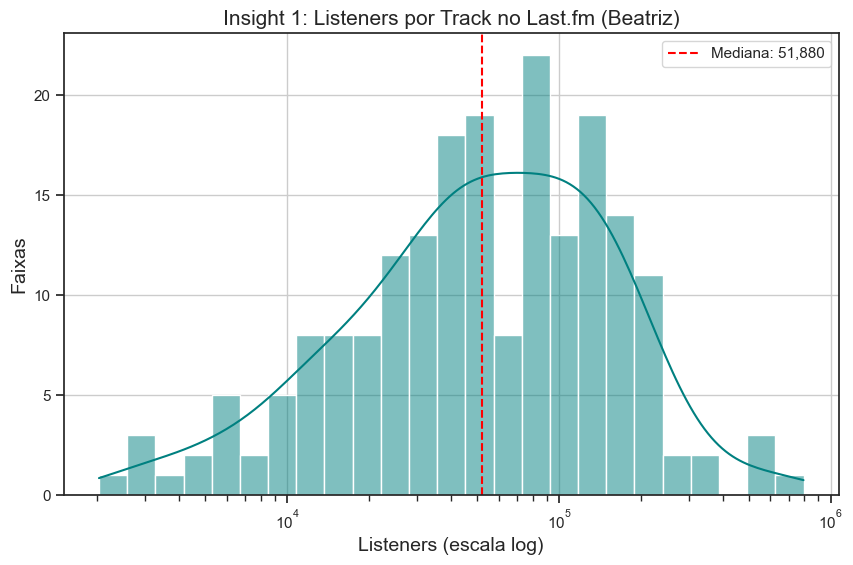
\includegraphics[width=0.78\textwidth]{beatriz_1_listeners.png}
\fontefig{Elaborado pelo autor (2026).}
\label{fig:beatriz-1}
\end{figure}

\begin{figure}[H]
\centering
\caption{Beatriz (input): distribuição de gêneros (\emph{top tags}).}
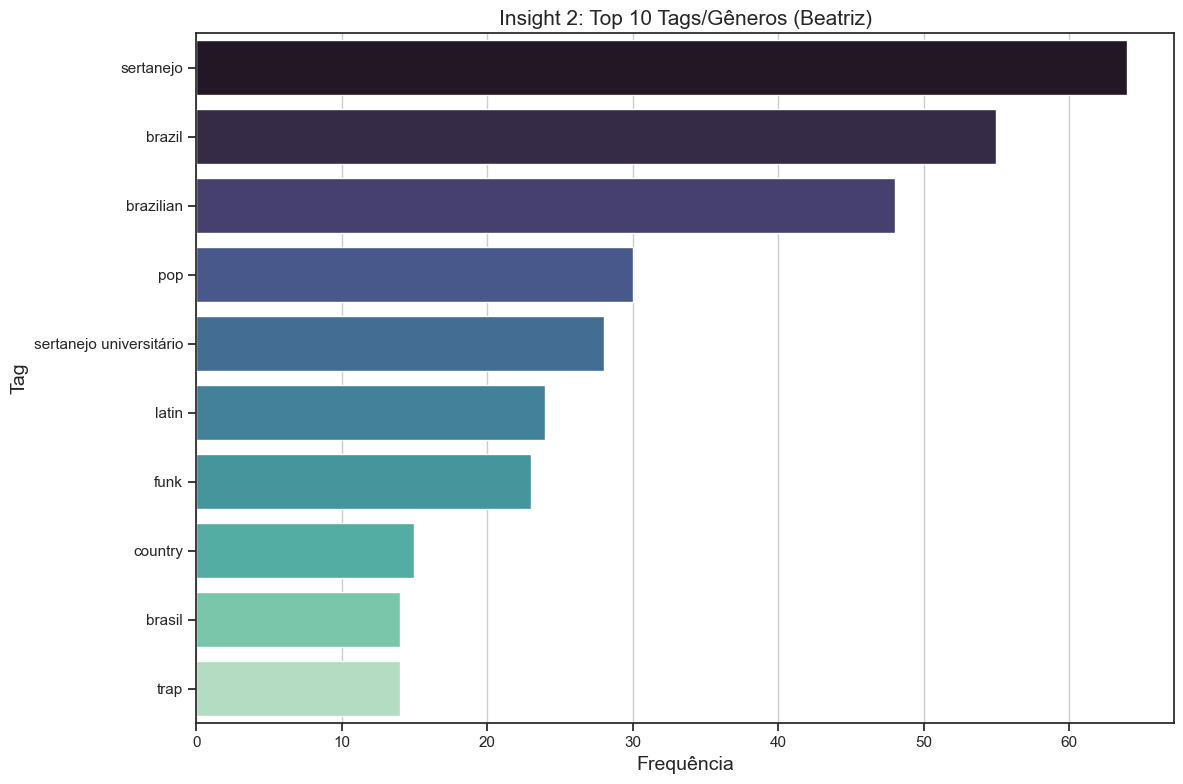
\includegraphics[width=0.78\textwidth]{beatriz_2_generos.png}
\fontefig{Elaborado pelo autor (2026).}
\label{fig:beatriz-2}
\end{figure}

\begin{figure}[H]
\centering
\caption{Beatriz (input): distribuição temporal (era musical das faixas).}
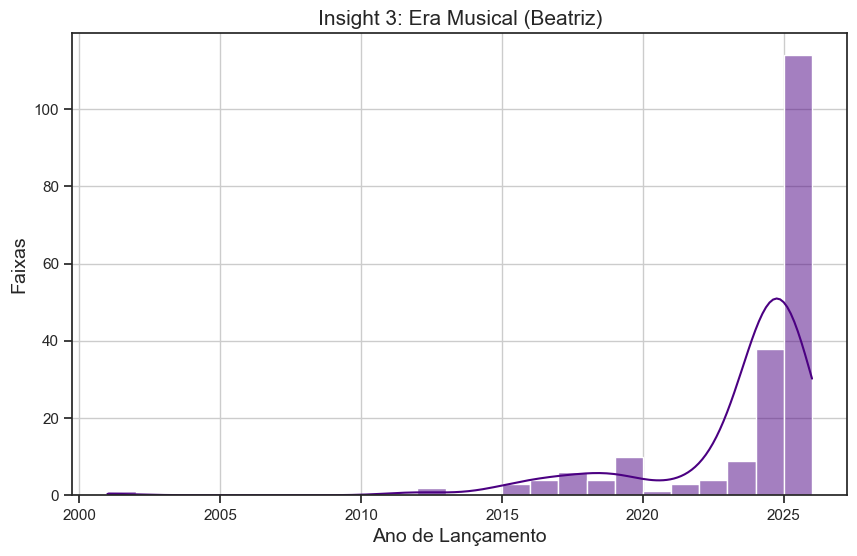
\includegraphics[width=0.78\textwidth]{beatriz_3_era.png}
\fontefig{Elaborado pelo autor (2026).}
\label{fig:beatriz-3}
\end{figure}

\begin{figure}[H]
\centering
\caption{Beatriz (input): concentração de artistas (Curva de Lorenz).}
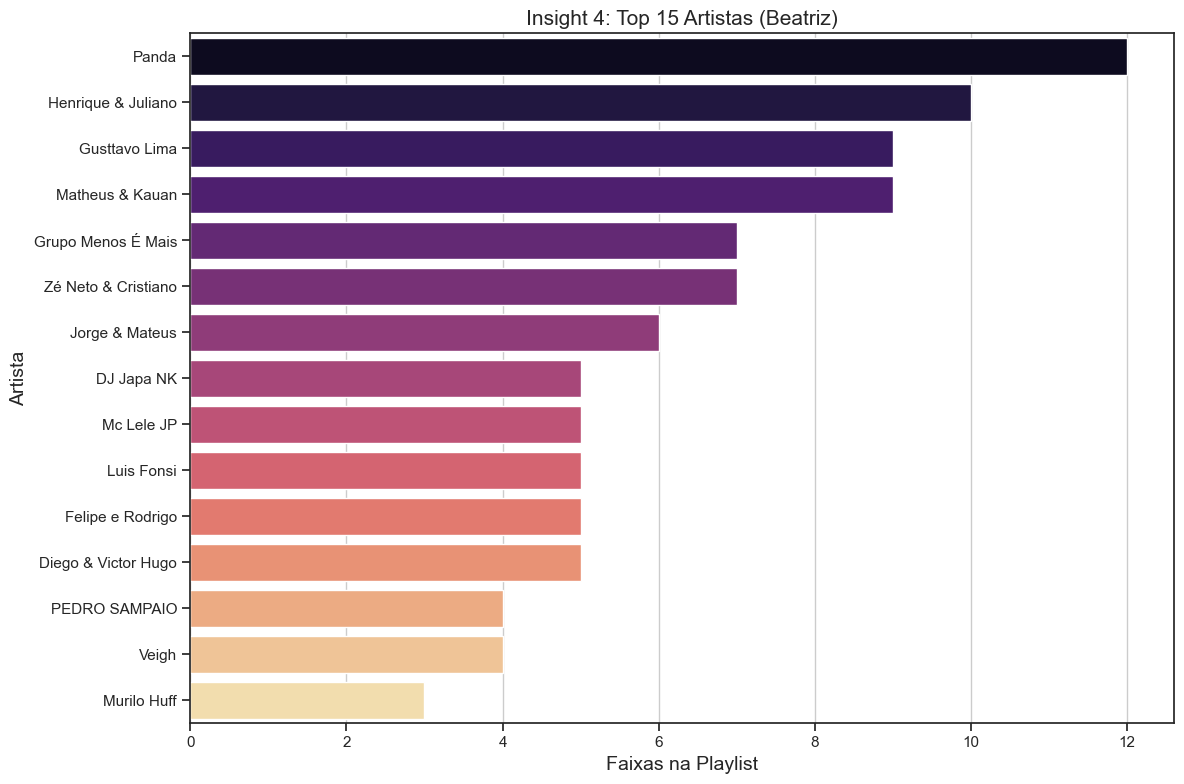
\includegraphics[width=0.78\textwidth]{beatriz_4_lorenz.png}
\fontefig{Elaborado pelo autor (2026).}
\label{fig:beatriz-4}
\end{figure}

\begin{figure}[H]
\centering
\caption{Beatriz (input): popularidade vs.\ alcance dos artistas.}
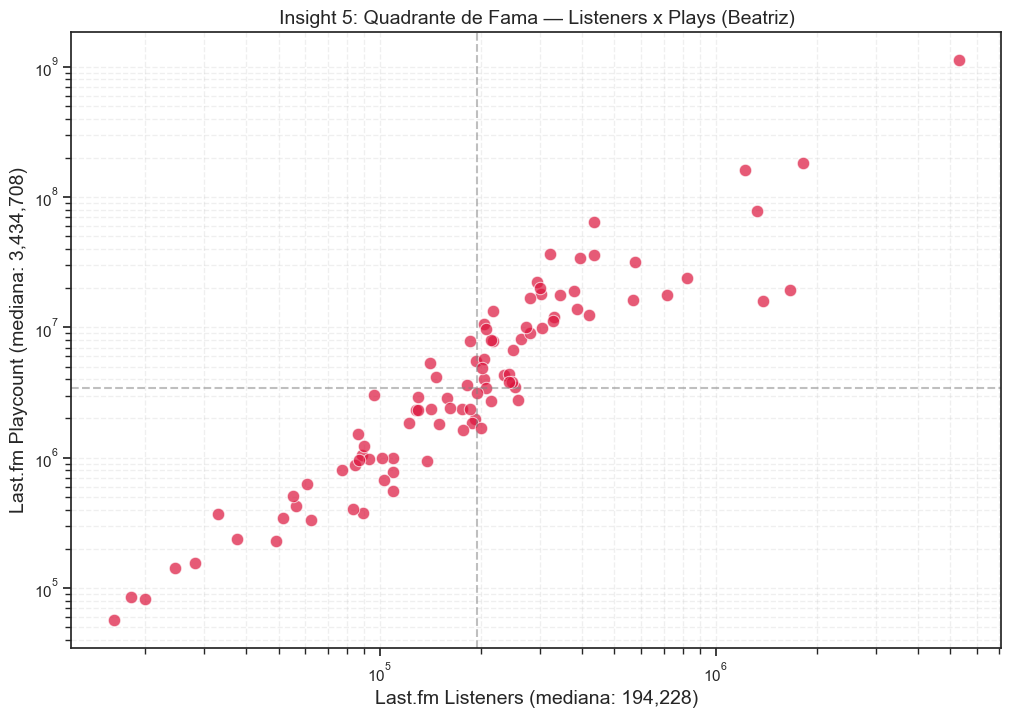
\includegraphics[width=0.85\textwidth]{beatriz_5_popfollow.png}
\fontefig{Elaborado pelo autor (2026).}
\label{fig:beatriz-5}
\end{figure}

\begin{figure}[H]
\centering
\caption{Beatriz (input): distribuição de duração das faixas.}
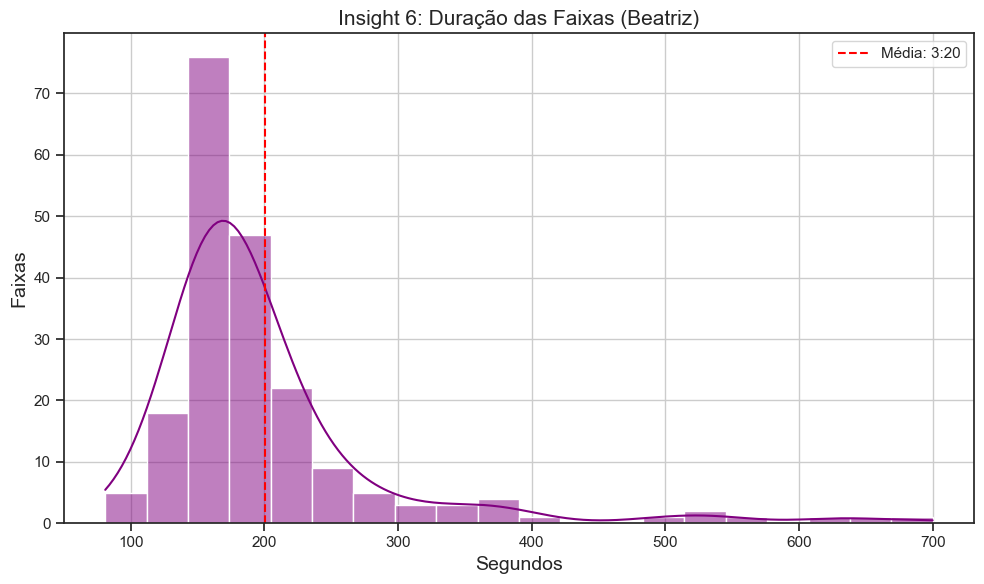
\includegraphics[width=0.78\textwidth]{beatriz_6_duracao.png}
\fontefig{Elaborado pelo autor (2026).}
\label{fig:beatriz-6}
\end{figure}

\subsection{Daniel (O Foco Instrumental/Lo-fi)}

\textbf{Perfil Psicográfico.} Sempre pragmático e focado, Daniel nunca encarou a
música como um componente central de sua identidade cultural, mas sim como uma
infraestrutura cognitiva. Formado em Ciência da Computação, foi durante a
graduação que descobriu o poder das paisagens sonoras como ferramenta de
produtividade. Atualmente com 25 anos e atuando como desenvolvedor de
\emph{software}, seu consumo musical é estritamente utilitário. Sua busca na
plataforma não é por artistas ou ídolos, mas por ``funções'': sonoridades para
concentração profunda (\emph{deep work}), batidas de baixa interferência para
programação ou frequências relaxantes. Para Daniel, a música não é uma obra de
arte a ser contemplada, mas um recurso \emph{bio-hackeável} para otimizar
desempenho e modulação de humor.

\textbf{Motivação Científica.} Esta persona foi desenhada para testar a
capacidade dos algoritmos de respeitarem contextos funcionais em detrimento da
popularidade. Daniel investiga o fenômeno da ``Música de Mobília''
(\emph{Furniture Music}), onde a faixa serve como plano de fundo. A hipótese
central é verificar se o sistema consegue manter a recomendação dentro de
parâmetros acústicos específicos (alta instrumentalidade, baixa energia, sem
vocais) ou se ocorrerá uma ``contaminação \emph{Pop}'', onde o algoritmo tenta
inserir faixas com vocais ou artistas famosos que quebram o fluxo de
concentração, revelando uma incapacidade de distinguir ``gosto musical'' de ``uso
funcional''.

\textbf{Validação Quantitativa do Input (Linha de Base).} Os dados de entrada
confirmam a construção de um perfil altamente especializado e, paradoxalmente,
anônimo. A biblioteca de Daniel apresenta uma \textbf{Mediana de Listeners por
Artista de 79,6 mil} (Last.fm), patamar característico da Cauda Longa do
consumo musical, combinada com uma \textbf{Mediana de Listeners por Track de
apenas 18,8 mil}. Esse contraste valida o fenômeno da Comoditização Musical: o
usuário consome o ``gênero'' (\emph{Lo-fi Beats}), ignorando completamente quem é
o autor da obra.

A estrutura das faixas é radicalmente distinta do padrão \emph{mainstream}. Com
\textbf{Duração Média de apenas 2:17}, as músicas são projetadas para
\emph{looping} contínuo e consumo rápido em \emph{playlists} de estudo. O viés de
recência é o mais extremo do estudo: \textbf{98,5\% das faixas pertencem à década
de 2020} (Ano Médio 2024), evidenciando a natureza efêmera e industrial desse
gênero, onde milhares de \emph{beats} são lançados diariamente para alimentar
algoritmos de foco.

A análise de \emph{tags} revela um \textbf{\emph{mono-cluster} temático}: as
marcas \texttt{lo-fi} (93 ocorrências), \texttt{hip hop} (83),
\texttt{downtempo} (78) e \texttt{instrumental} (77) dominam massivamente. A
predominância de \textbf{70\% artistas solo (\emph{Person})} confirma o
ecossistema de \emph{bedroom producers}, produtores independentes que operam
em isolamento, contribuindo individualmente para o catálogo \emph{lo-fi}
industrial. A \textbf{Era de Carreira Mediana de 1987} (cobertura limitada: 20\%,
refletindo a invisibilidade de produtores obscuros nos catálogos do MusicBrainz)
deve ser interpretada com cautela.

\begin{table}[H]
\centering
\caption{Indicadores quantitativos do perfil Daniel (input).}
\label{tab:daniel}
\footnotesize
\begin{tabularx}{\textwidth}{>{\raggedright\arraybackslash}p{4.3cm} >{\raggedright\arraybackslash}p{2.6cm} X}
\toprule
\textbf{Indicador} & \textbf{Valor Obtido} & \textbf{Interpretação Científica} \\
\midrule
Listeners Mediano por Artista (Last.fm) & 79.595 & Zona de Cauda Longa: base de fãs ativa baixa, mas \emph{plays} altos via consumo passivo. \\
Playcount Mediano por Artista (Last.fm) & 348.630 & Histórico cumulativo modesto, característico da era \emph{streaming} funcional. \\
Listeners Mediano por Track (Last.fm) & 18.824 & Faixas projetadas para \emph{background listening}, sem aspiração a \emph{hit} cultural. \\
Entropia de Shannon (Artistas) & 6,27 (Máxima do estudo) & Pulverização Funcional; indiferença à autoria, consome-se o ``gênero'', não o ``artista''. \\
Coeficiente de Gini & 0,37 (Baixo-Médio) & Pouca concentração; distribuição quase uniforme entre os 99 produtores. \\
Riqueza (Artistas Únicos) & 99 (média 2,02 faixas/artista) & Consumo extremamente disperso. \\
Era de Carreira Mediana & 1987 (cob.\ 20\%) & Cobertura limitada, muitos produtores \emph{lo-fi} sem registro no MusicBrainz; baixa confiabilidade. \\
Tipo de Artista (MB) & 70\% solo, 24\% grupo & Confirma ecossistema de \emph{bedroom producers} individuais. \\
Recência Temporal (Álbum) & 98,5\% Anos 2020 & Produção Industrial/Efêmera; obsolescência rápida do catálogo. \\
Tags Dominantes (mb+lastfm) & lo-fi, hip hop, downtempo, instrumental & Hiper-especialização cognitiva; bloqueio de vocais e dinâmicas intensas (\emph{Deep Work}). \\
HHI de Tags & 0,055 (Baixo) & Tags concentradas em poucos termos do mesmo \emph{cluster} sonoro. \\
Estrutura (Duração) & Média 2:17 & Economia do \emph{Stream}; \emph{looping} contínuo em sessões longas. \\
\bottomrule
\end{tabularx}
\fontefig{Elaborado pelo autor (2026).}
\end{table}

Os seis painéis de Daniel evidenciam seu perfil funcional. A distribuição de
\emph{listeners} por faixa (Figura~\ref{fig:daniel-1}) desloca-se para valores
baixos ($\approx$18,8 mil), típicos de \emph{background listening}; o mapa de
gêneros (Figura~\ref{fig:daniel-2}) revela o \emph{mono-cluster}
\texttt{lo-fi}/\texttt{instrumental}/\texttt{downtempo}; a distribuição temporal
(Figura~\ref{fig:daniel-3}) é a mais concentrada nos anos 2020 do estudo
(98,5\%), refletindo a produção industrial e efêmera do gênero; a Curva de Lorenz
(Figura~\ref{fig:daniel-4}) é quase diagonal (Gini 0,37), confirmando a
pulverização entre produtores; o cruzamento de audiência
(Figura~\ref{fig:daniel-5}) situa Daniel na zona de cauda longa; e a distribuição
de duração (Figura~\ref{fig:daniel-6}) concentra-se em torno de 2:17, otimizada
para \emph{looping}.

\begin{figure}[H]
\centering
\caption{Daniel (input): distribuição de \emph{listeners} por faixa (Last.fm).}
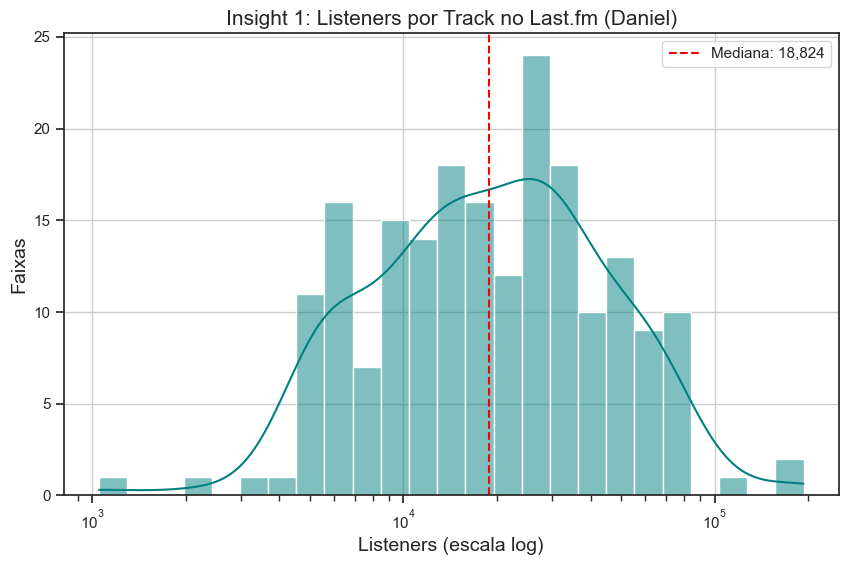
\includegraphics[width=0.78\textwidth]{daniel_1_listeners.png}
\fontefig{Elaborado pelo autor (2026).}
\label{fig:daniel-1}
\end{figure}

\begin{figure}[H]
\centering
\caption{Daniel (input): distribuição de gêneros (\emph{top tags}).}
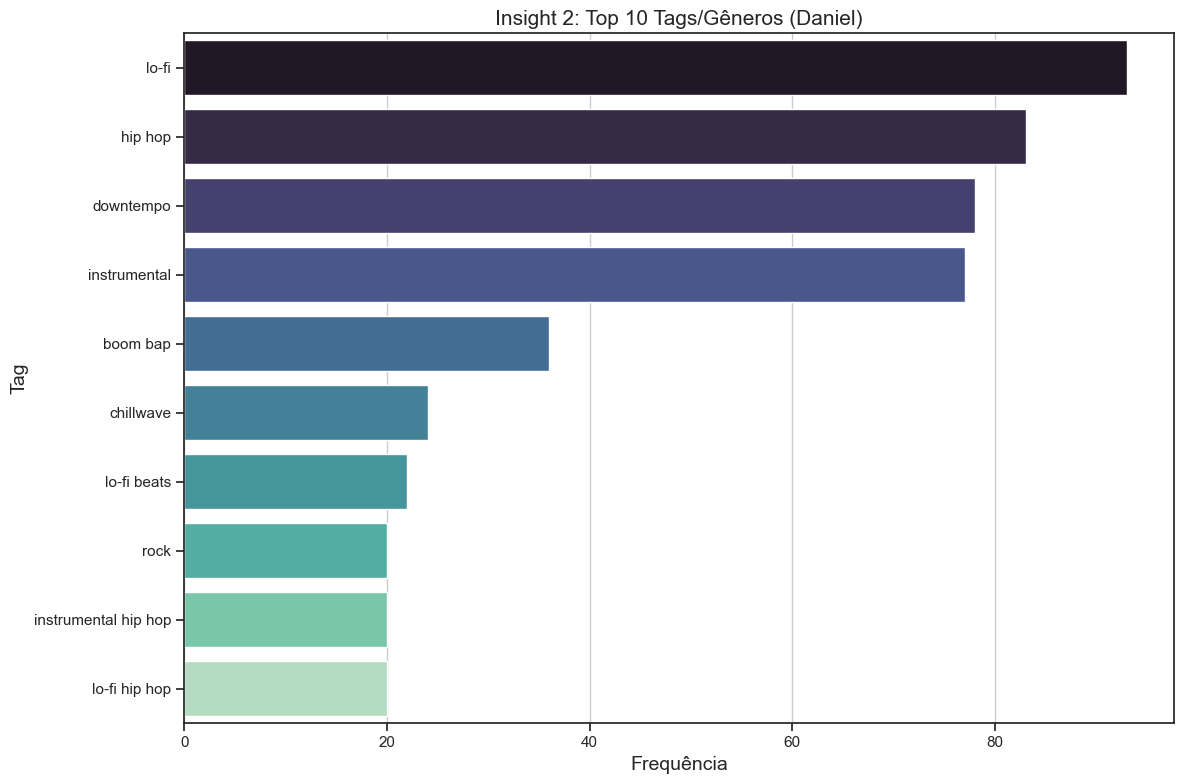
\includegraphics[width=0.78\textwidth]{daniel_2_generos.png}
\fontefig{Elaborado pelo autor (2026).}
\label{fig:daniel-2}
\end{figure}

\begin{figure}[H]
\centering
\caption{Daniel (input): distribuição temporal (era musical das faixas).}
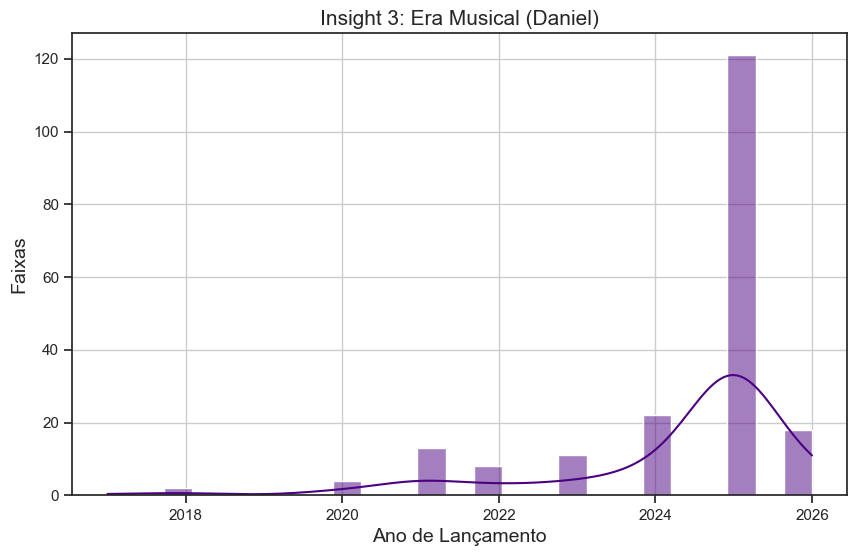
\includegraphics[width=0.78\textwidth]{daniel_3_era.png}
\fontefig{Elaborado pelo autor (2026).}
\label{fig:daniel-3}
\end{figure}

\begin{figure}[H]
\centering
\caption{Daniel (input): concentração de artistas (Curva de Lorenz).}
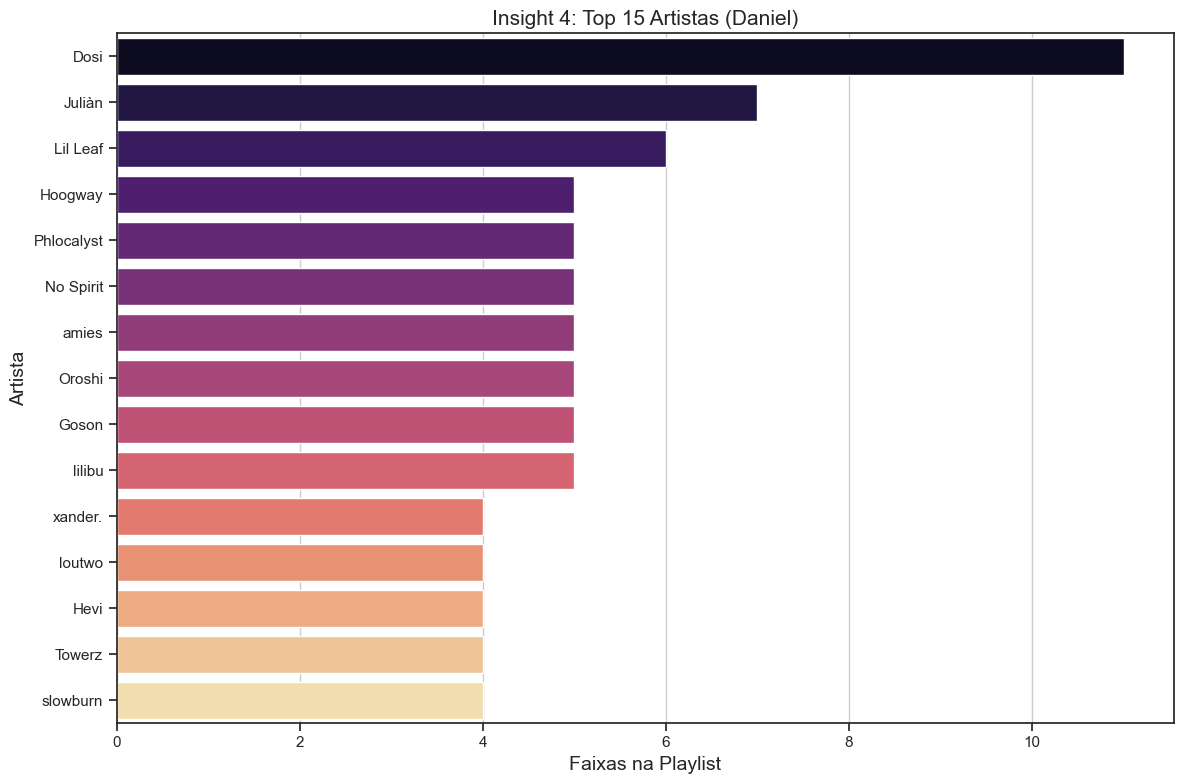
\includegraphics[width=0.78\textwidth]{daniel_4_lorenz.png}
\fontefig{Elaborado pelo autor (2026).}
\label{fig:daniel-4}
\end{figure}

\begin{figure}[H]
\centering
\caption{Daniel (input): popularidade vs.\ alcance dos artistas.}
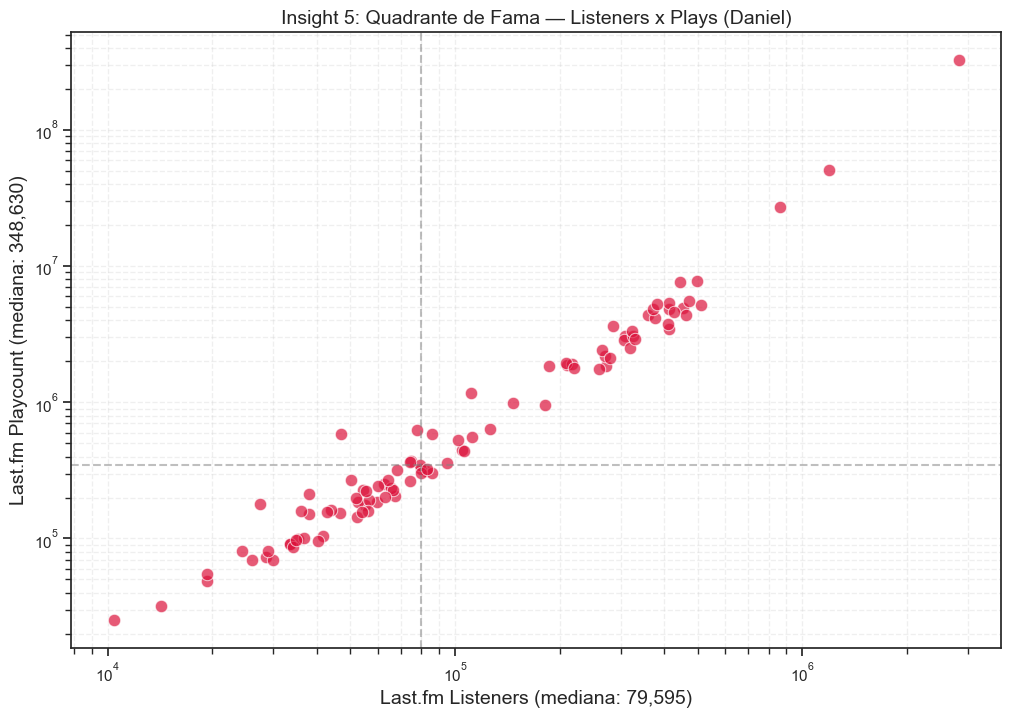
\includegraphics[width=0.85\textwidth]{daniel_5_popfollow.png}
\fontefig{Elaborado pelo autor (2026).}
\label{fig:daniel-5}
\end{figure}

\begin{figure}[H]
\centering
\caption{Daniel (input): distribuição de duração das faixas.}
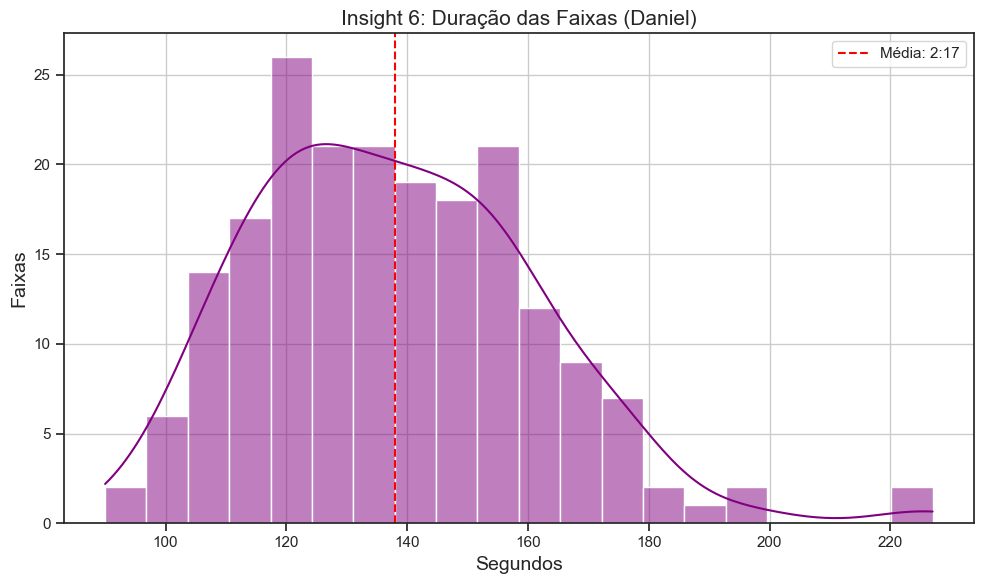
\includegraphics[width=0.78\textwidth]{daniel_6_duracao.png}
\fontefig{Elaborado pelo autor (2026).}
\label{fig:daniel-6}
\end{figure}

\subsection{Sofia (A Consumidora de Nicho)}

\textbf{Perfil Psicográfico.} Nascida em 2002, Sofia cresceu na fronteira entre o
físico e o digital, mas escolheu habitar os cantos mais silenciosos da internet.
Formada em Design Gráfico, ela encara a música não como entretenimento de fundo,
mas como uma extensão direta de sua identidade estética e emocional. Diferente da
euforia coletiva de Beatriz, a experiência musical de Sofia é introspectiva e
solitária, forjada em fóruns de discussão e \emph{blogs} especializados (como o
Rate Your Music) em vez de \emph{feeds} de redes sociais de massa. Ela valoriza a
autenticidade, a textura sonora e a ``melancolia poética'', buscando ativamente o
que é raro. Sua postura é de curadoria ativa: Sofia não espera que o algoritmo
lhe diga o que ouvir; ela garimpa, cataloga e preserva suas descobertas como
artefatos digitais preciosos, temendo a banalização de seus ``tesouros'' pelo
\emph{mainstream}.

\textbf{Motivação.} Esta persona atua como o Caso de Borda (\emph{Edge Case}) ou
o teste da Cauda Longa (\emph{Long Tail}). Sofia representa o desafio de
personalização para usuários com gostos altamente específicos e baixa
sobreposição com a massa de dados global. O objetivo é testar a capacidade do
sistema de recomendação em operar com \emph{data sparsity} (escassez de dados
comportamentais coletivos), verificando se o algoritmo consegue manter a
coerência estética de nicho ou se sofre de um viés de popularidade, sugerindo
artistas famosos incorretamente na tentativa de preencher lacunas. Avalia-se aqui
a precisão em micro-gêneros e a sensibilidade a texturas sonoras complexas.

\textbf{Validação Quantitativa do Input.} A análise dos metadados da biblioteca
de Sofia confirma rigorosamente seu arquétipo de ``Arqueóloga Digital'' e
consumidora \emph{underground}. A Mediana de Listeners por Track no Last.fm é de
apenas \textbf{1.223}, três ordens de magnitude abaixo de Beatriz (51.879) e
quase 16 vezes menor que Daniel, evidenciando que a grande maioria de seu
consumo reside na obscuridade quase total do catálogo global. A Mediana de
Listeners por Artista (59.042) também é a mais baixa do estudo, validando seu
interesse pelo cenário independente.

O comportamento de consumo de Sofia é profundamente focado e leal, evidenciado
pela \textbf{média de 7,41 faixas por artista} (segunda maior, atrás apenas de
Ricardo). Enquanto a persona \emph{mainstream} consome \emph{hits} isolados,
Sofia consome discografias e álbuns: artistas como S.Maharba, Eterna e Patch+
possuem 15 ou mais faixas cada em sua biblioteca, demonstrando uma escuta
vertical e investigativa.

Temporalmente, ela compartilha o viés de contemporaneidade (Ano Médio 2021, com
77\% das faixas na década de 2020), mas com um propósito diferente: ela busca a
vanguarda experimental atual, não os sucessos de rádio. A distribuição de
\emph{tags} valida sua formação em design e gosto por atmosferas: há
predominância de estilos baseados em textura e colagem sonora, 
\texttt{shoegaze}, \texttt{plunderphonics}, \texttt{cloud rap}, \texttt{IDM},
\texttt{lo-fi indie}, gêneros complexos que exigem análise de conteúdo de
áudio (timbre/ritmo) mais apurada do que a simples filtragem colaborativa. A
composição \textbf{61\% solo, 39\% grupos} (MusicBrainz) reflete a predominância
individual típica de cenas independentes contemporâneas.

\begin{table}[H]
\centering
\caption{Indicadores quantitativos do perfil Sofia (input).}
\label{tab:sofia}
\footnotesize
\begin{tabularx}{\textwidth}{>{\raggedright\arraybackslash}p{4.3cm} >{\raggedright\arraybackslash}p{2.6cm} X}
\toprule
\textbf{Indicador} & \textbf{Valor Obtido} & \textbf{Interpretação Científica} \\
\midrule
Listeners Mediano por Artista (Last.fm) & 59.042 & A mais baixa do estudo; isolamento quase total das tendências de massa. \\
Playcount Mediano por Artista (Last.fm) & 565.579 & Comunidades de nicho com fãs leais e ativos, gerando \emph{plays} concentrados em audiência pequena. \\
Listeners Mediano por Track (Last.fm) & \textbf{1.223} & \textbf{Três ordens de magnitude abaixo do \emph{mainstream}}; consumo na obscuridade extrema do catálogo global. \\
Entropia de Shannon (Artistas) & 4,43 (Baixa) & Consumo Imersivo/Vertical; forte oposição à escuta passiva. \\
Coeficiente de Gini & 0,36 & Distribuição com algumas favoritas claras (S.Maharba, Eterna, Patch+ com 15+ faixas cada). \\
Riqueza (Artistas Únicos) & 27 (média 7,41 faixas/artista) & Escuta focada em discografia profunda, \emph{active listening}. \\
Era de Carreira Mediana & 1984 (cob.\ 41\%) & Cena experimental com mistura de pioneiros (anos 80--90) e contemporâneos. \\
Tipo de Artista (MB) & 61\% solo, 39\% grupo & Predominância de projetos individuais, característico de cenas independentes. \\
Recência Temporal (Álbum) & 77,0\% Anos 2020 & Vanguarda contemporânea; busca do alternativo no tempo presente. \\
Tags Dominantes (mb+lastfm) & shoegaze, plunderphonics, cloud rap, IDM, lo-fi indie & Curadoria estético-textural; gêneros de alta complexidade tímbrica. \\
HHI de Tags & 0,024 (Mais baixo do estudo) & Maior diversidade tímbrica/conceitual entre as personas. \\
Estrutura (Duração) & Média 2:57 (\emph{range} 0:06--7:04) & Flexibilidade artística; rejeição à padronização (vinhetas a épicos). \\
\bottomrule
\end{tabularx}
\fontefig{Elaborado pelo autor (2026).}
\end{table}

Os seis painéis de Sofia confirmam o arquétipo \emph{underground}. A distribuição
de \emph{listeners} por faixa (Figura~\ref{fig:sofia-1}) é a mais deslocada para
a obscuridade (mediana de 1.223), três ordens de magnitude abaixo do
\emph{mainstream}; o mapa de gêneros (Figura~\ref{fig:sofia-2}) reúne estilos
texturais (\texttt{shoegaze}, \texttt{plunderphonics}, \texttt{IDM}); a
distribuição temporal (Figura~\ref{fig:sofia-3}) é contemporânea, porém de
vanguarda; a Curva de Lorenz (Figura~\ref{fig:sofia-4}) reflete a escuta vertical
em poucos artistas favoritos; o cruzamento de audiência
(Figura~\ref{fig:sofia-5}) posiciona-a no quadrante de nicho; e a distribuição de
duração (Figura~\ref{fig:sofia-6}) é a mais ampla do estudo (0:06 a 7:04),
evidenciando rejeição à padronização.

\begin{figure}[H]
\centering
\caption{Sofia (input): distribuição de \emph{listeners} por faixa (Last.fm).}
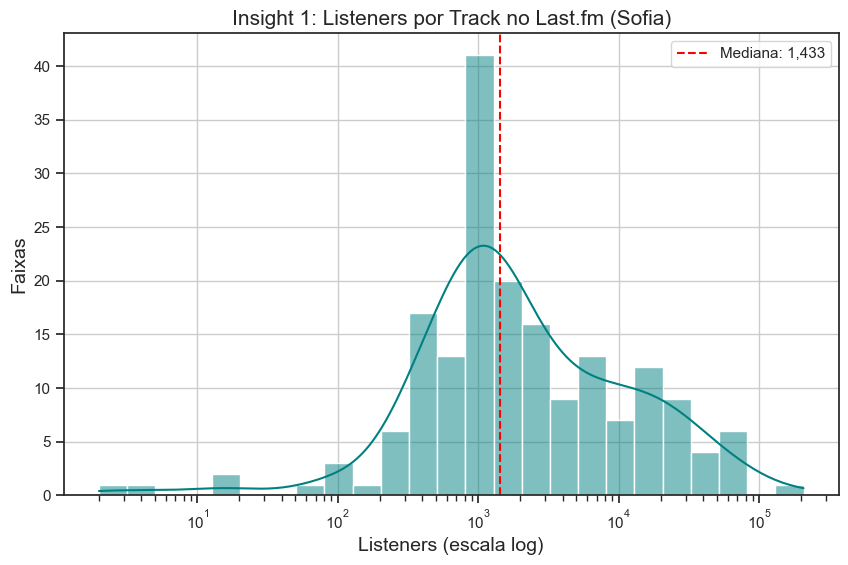
\includegraphics[width=0.78\textwidth]{sofia_1_listeners.png}
\fontefig{Elaborado pelo autor (2026).}
\label{fig:sofia-1}
\end{figure}

\begin{figure}[H]
\centering
\caption{Sofia (input): distribuição de gêneros (\emph{top tags}).}
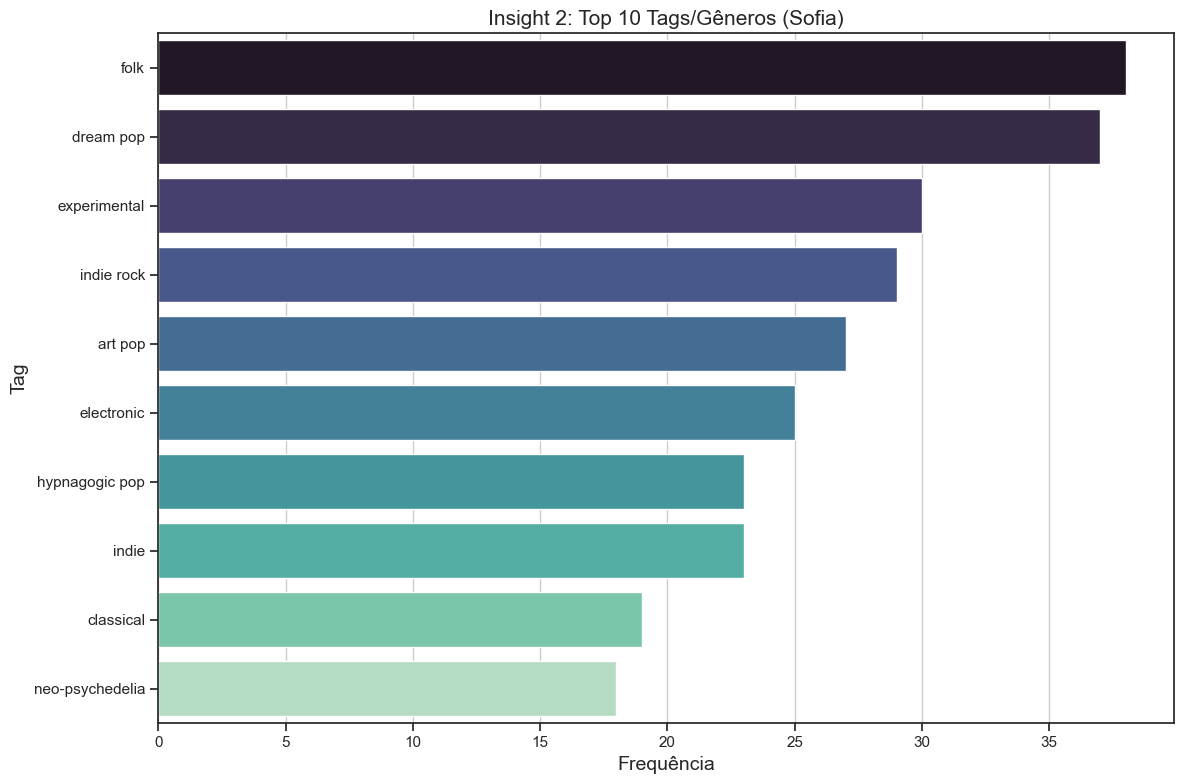
\includegraphics[width=0.78\textwidth]{sofia_2_generos.png}
\fontefig{Elaborado pelo autor (2026).}
\label{fig:sofia-2}
\end{figure}

\begin{figure}[H]
\centering
\caption{Sofia (input): distribuição temporal (era musical das faixas).}
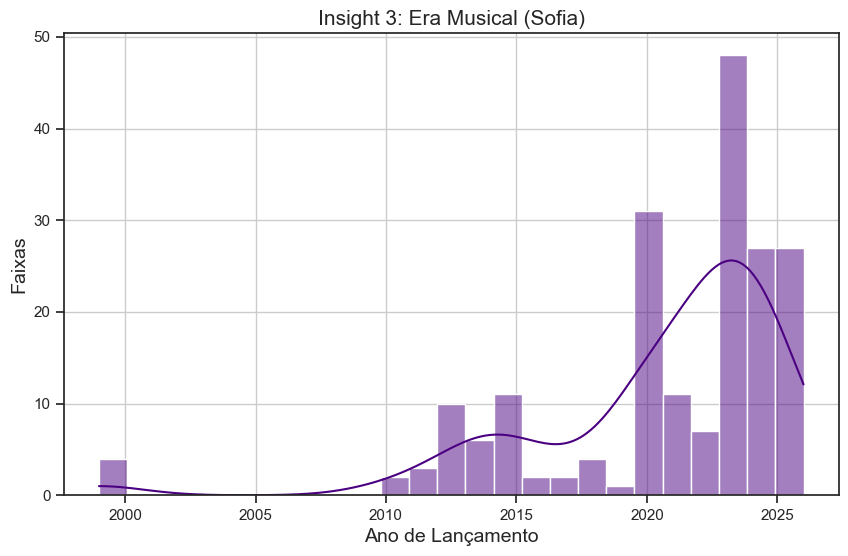
\includegraphics[width=0.78\textwidth]{sofia_3_era.png}
\fontefig{Elaborado pelo autor (2026).}
\label{fig:sofia-3}
\end{figure}

\begin{figure}[H]
\centering
\caption{Sofia (input): concentração de artistas (Curva de Lorenz).}
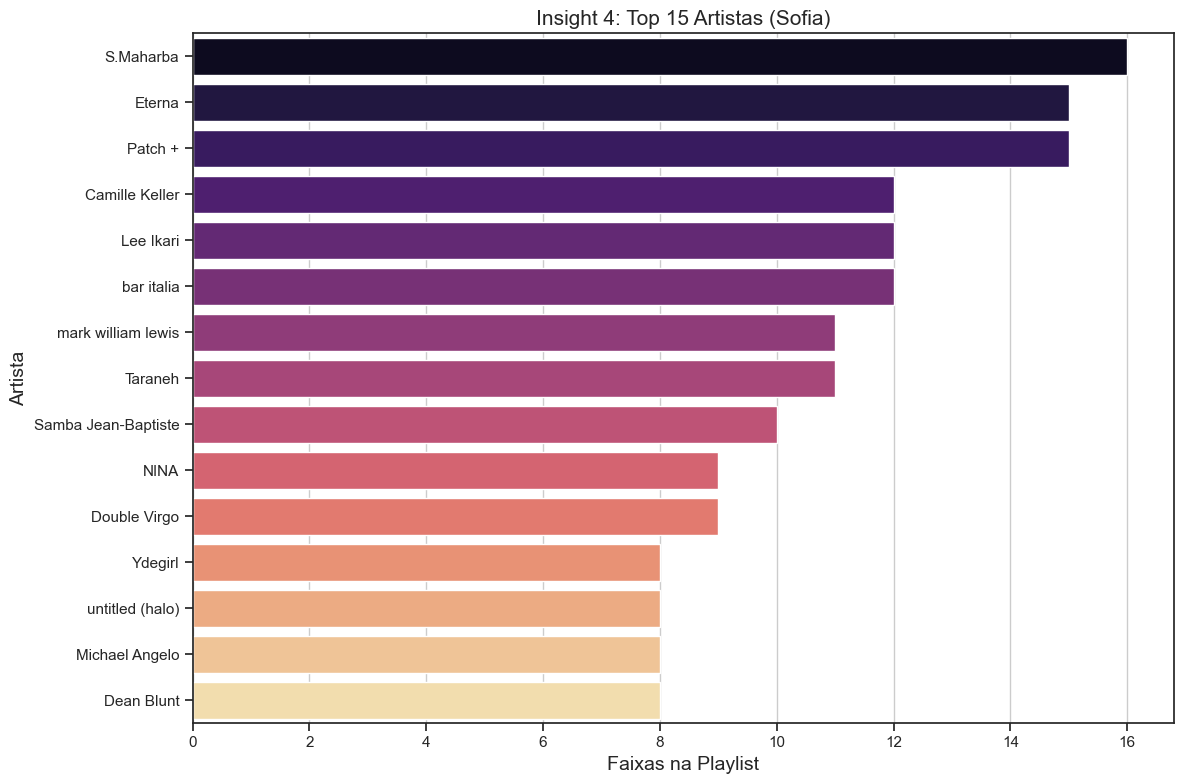
\includegraphics[width=0.78\textwidth]{sofia_4_lorenz.png}
\fontefig{Elaborado pelo autor (2026).}
\label{fig:sofia-4}
\end{figure}

\begin{figure}[H]
\centering
\caption{Sofia (input): popularidade vs.\ alcance dos artistas.}
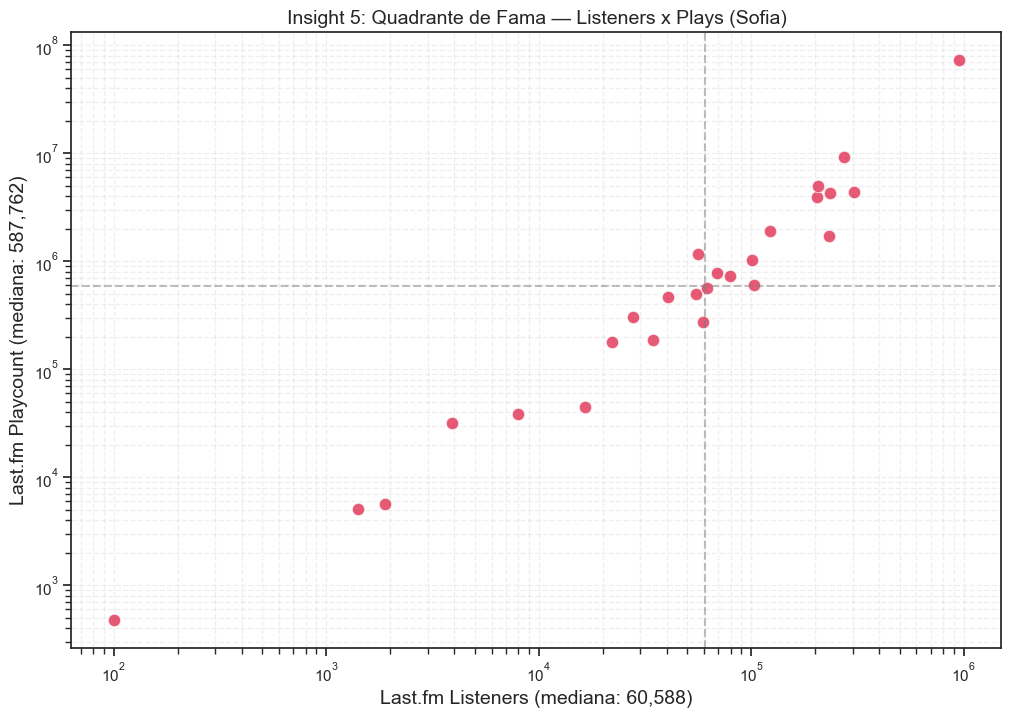
\includegraphics[width=0.85\textwidth]{sofia_5_popfollow.png}
\fontefig{Elaborado pelo autor (2026).}
\label{fig:sofia-5}
\end{figure}

\begin{figure}[H]
\centering
\caption{Sofia (input): distribuição de duração das faixas.}
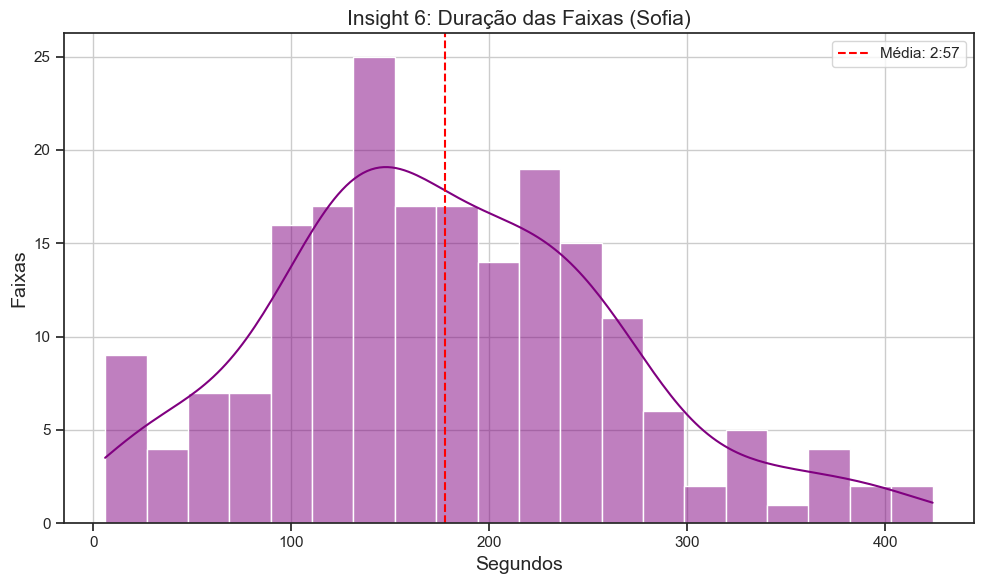
\includegraphics[width=0.78\textwidth]{sofia_6_duracao.png}
\fontefig{Elaborado pelo autor (2026).}
\label{fig:sofia-6}
\end{figure}

\subsection{Ricardo (O Consumidor Nostálgico)}

\textbf{Perfil Psicográfico.} Nascido em 1982, Ricardo representa a transição da
era analógica para a digital. Sua formação musical ocorreu na ``Era de Ouro'' da
indústria fonográfica física (anos 90), moldada pela escassez e pela valorização
do objeto: a gravação de fitas K7, a compra ritualística de LPs e a apreciação de
álbuns completos. Como Engenheiro Civil, ele possui uma abordagem estruturada e
crítica em relação ao consumo; para ele, a música deve possuir narrativa,
complexidade instrumental e autenticidade técnica. Embora utilize o
\emph{streaming} por conveniência, sua mentalidade permanece a de um colecionador.
Ricardo exibe uma forte resistência algorítmica: ele desconfia da superficialidade
das ``curadorias automáticas'' e prefere atuar como o guardião do ``bom gosto'' em
seu círculo social, utilizando momentos de lazer (como churrascos) para educar as
gerações mais novas sobre os clássicos do Rock e da MPB.

\textbf{Motivação.} Esta persona atua como o Controle Temporal (\emph{Legacy
Control}) do experimento. Ricardo desafia o sistema de recomendação a lidar com o
``Viés de Recência'' (\emph{Recency Bias}). O objetivo é verificar se o algoritmo
consegue distinguir entre ``Alta Popularidade Atual'' e ``Alta Popularidade
Histórica''. Testa-se a capacidade do modelo em recomendar ``\emph{Deep Cuts}''
(faixas menos conhecidas de artistas famosos) e se ele é capaz de sair do
\emph{loop} temporal, sugerindo, por exemplo, bandas novas que tenham a sonoridade
``\emph{Classic Rock}'' (Greta Van Fleet, por exemplo) ou se ficará preso
recomendando apenas reedições das décadas de 70 e 80, gerando um estagnamento de
descoberta.

\textbf{Validação Quantitativa do Input.} A análise dos metadados valida
robustamente o arquétipo do ouvinte ``Saudosista e Leal''. A biblioteca exibe a
\textbf{Mediana de Listeners por Artista mais alta do estudo}, \textbf{4,4
milhões} no Last.fm, e uma \textbf{Mediana de Playcount Histórico cumulativo
de 144,5 milhões}, evidenciando que Ricardo consome ``Lendas da Música'' e
``Gigantes do Estádio'' (Metallica, Queen, Rolling Stones, Beatles). A
\textbf{Mediana de Listeners por Track de 311 mil} corrobora que mesmo as faixas
individuais escolhidas são \emph{singles} de grande exposição.

O indicador mais forte de seu comportamento de ``escuta de álbum'' (em oposição à
escuta de \emph{playlist}) é a \textbf{Concentração de Artistas}: com apenas
\textbf{18 artistas únicos para 200 músicas} (média 11,11 faixas/artista),
Ricardo apresenta a \textbf{menor entropia de Shannon do estudo (4,10) e Gini de
0,18} (mínimo de desigualdade, todos os 18 artistas têm peso comparável). Isso
confirma que ele não consome apenas os \emph{greatest hits}, mas mergulha na
discografia profunda de seus ídolos (ex.: 16 faixas de Djavan e Metallica).

Temporalmente, o \emph{input} é deslocado para o século passado, com Ano Médio de
Lançamento de 1985 e mais de 81\% das faixas concentradas entre as décadas de 70,
80 e 90. A análise de \textbf{Era de Carreira no MusicBrainz} (cobertura 100\%, 
todos os 18 artistas têm registro completo) confirma com \textbf{mediana de 1965}
que a seleção concentra-se em artistas que iniciaram carreira na ``Era de Ouro''
da indústria fonográfica. \textbf{66,7\% dos artistas são bandas (\emph{Group})},
refletindo a centralidade do \emph{band format} no rock clássico, em contraste
com a predominância solo das demais personas. Estruturalmente, a \emph{playlist}
rejeita a economia da atenção atual: Duração Média de 4:33, com faixas chegando a
quase 9 minutos.

\begin{table}[H]
\centering
\caption{Indicadores quantitativos do perfil Ricardo (input).}
\label{tab:ricardo}
\footnotesize
\begin{tabularx}{\textwidth}{>{\raggedright\arraybackslash}p{4.3cm} >{\raggedright\arraybackslash}p{2.6cm} X}
\toprule
\textbf{Indicador} & \textbf{Valor Obtido} & \textbf{Interpretação Científica} \\
\midrule
Listeners Mediano por Artista (Last.fm) & \textbf{4.412.516} & Zona de consagração histórica; o mais alto do estudo. Lendas globais com milhões de fãs. \\
Playcount Mediano por Artista (Last.fm) & \textbf{144.558.091} & Histórico cumulativo enorme, décadas de \emph{plays} acumulados. Validação canônica plena. \\
Listeners Mediano por Track (Last.fm) & 311.105 & \emph{Singles} consagrados; todas as faixas têm exposição internacional sustentada. \\
Entropia de Shannon (Artistas) & \textbf{4,10 (Mínima do estudo)} & Baixa \textbf{riqueza} (poucos artistas), não concentração: a \emph{evenness} de Pielou (0,98) confirma distribuição uniforme. \\
Coeficiente de Gini & \textbf{0,18 (Mínimo do estudo)} & Distribuição quase uniforme entre os 18 artistas, todos com 8--16 faixas. \\
Riqueza (Artistas Únicos) & \textbf{18 (média 11,11 faixas/artista)} & \emph{Album-Oriented Rock}, escuta de discografia, não de \emph{playlist}. \\
Era de Carreira Mediana (MB) & \textbf{1965 (cob.\ 100\%)} & Era de Ouro da indústria fonográfica; cobertura integral confirma artistas plenamente documentados. \\
Tipo de Artista (MB) & \textbf{66,7\% grupo, 33,3\% solo} & Predominância de bandas, refletindo o \emph{band format} do rock clássico. \\
Recência Temporal (Álbum) & Ano Médio 1985 ($>$81\% entre 70s--90s) & Cristalização temporal; viés de nostalgia ativo. \\
Tags Dominantes (mb+lastfm) & rock, classic rock, hard rock, MPB, bossa nova & Purismo analógico; instrumentação orgânica e virtuosismo técnico. \\
HHI de Tags & 0,054 & Concentração moderada; \emph{cluster} temático claro mas não monolítico. \\
Estrutura (Duração) & Média 4:33 (\emph{range} 2:02--8:35) & Narrativa progressiva; rejeição à economia da atenção atual. \\
\bottomrule
\end{tabularx}
\fontefig{Elaborado pelo autor (2026).}
\end{table}

Os seis painéis de Ricardo caracterizam o ouvinte de legado. A distribuição de
\emph{listeners} por faixa (Figura~\ref{fig:ricardo-1}) é a mais alta do estudo
(mediana de 311 mil), formada por \emph{singles} consagrados; o mapa de gêneros
(Figura~\ref{fig:ricardo-2}) concentra \texttt{rock}, \texttt{classic rock} e
\texttt{MPB}; a distribuição temporal (Figura~\ref{fig:ricardo-3}) isola-se no
século XX ($>$81\% entre as décadas de 70 e 90); a Curva de Lorenz
(Figura~\ref{fig:ricardo-4}) é a mais afastada da diagonal, refletindo a
fidelidade a apenas 18 artistas; o cruzamento de audiência
(Figura~\ref{fig:ricardo-5}) situa-o no quadrante \emph{Head} de máxima
consagração; e a distribuição de duração (Figura~\ref{fig:ricardo-6}) é a mais
longa (média 4:33), com faixas de quase 9 minutos.

\begin{figure}[H]
\centering
\caption{Ricardo (input): distribuição de \emph{listeners} por faixa (Last.fm).}
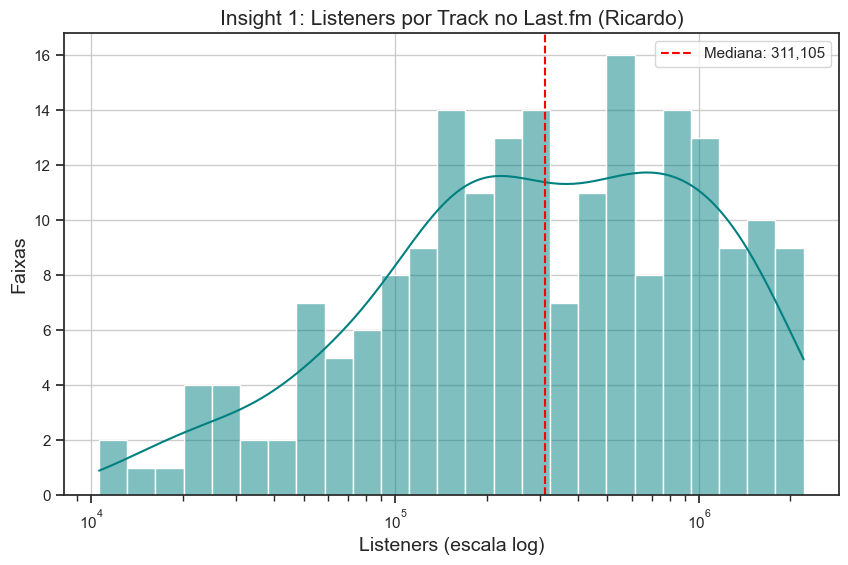
\includegraphics[width=0.78\textwidth]{ricardo_1_listeners.png}
\fontefig{Elaborado pelo autor (2026).}
\label{fig:ricardo-1}
\end{figure}

\begin{figure}[H]
\centering
\caption{Ricardo (input): distribuição de gêneros (\emph{top tags}).}
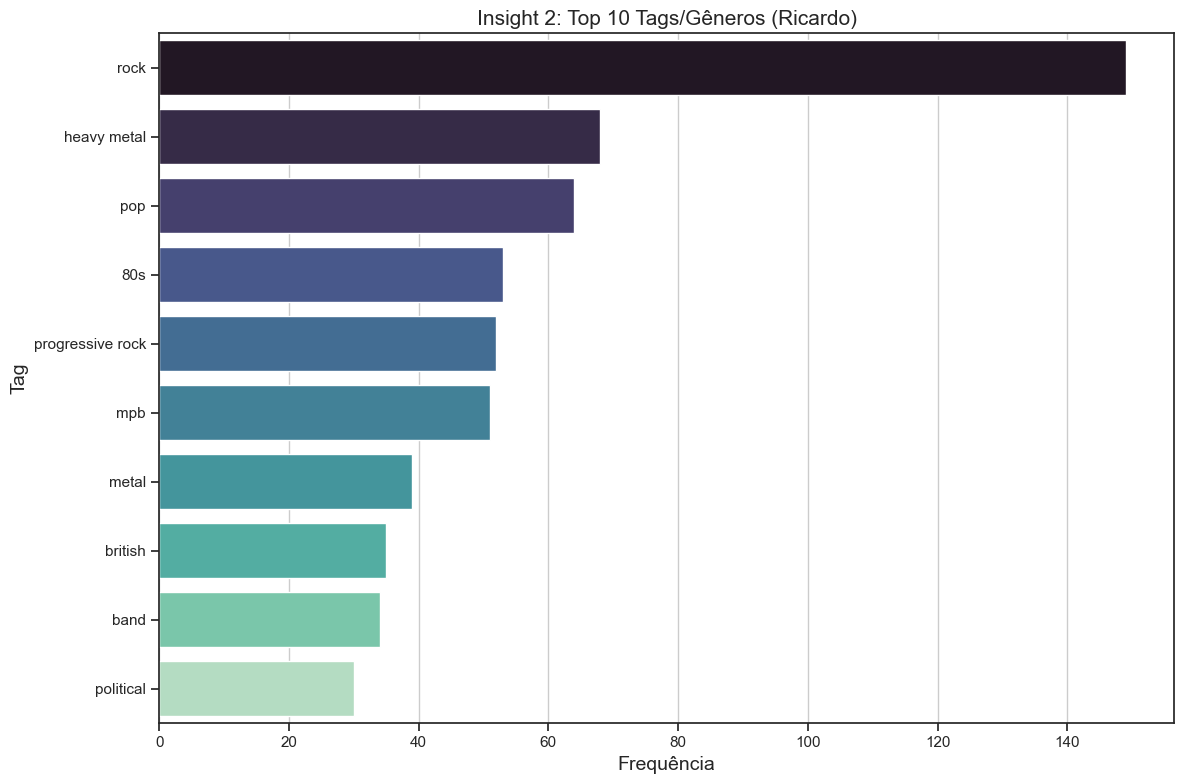
\includegraphics[width=0.78\textwidth]{ricardo_2_generos.png}
\fontefig{Elaborado pelo autor (2026).}
\label{fig:ricardo-2}
\end{figure}

\begin{figure}[H]
\centering
\caption{Ricardo (input): distribuição temporal (era musical das faixas).}
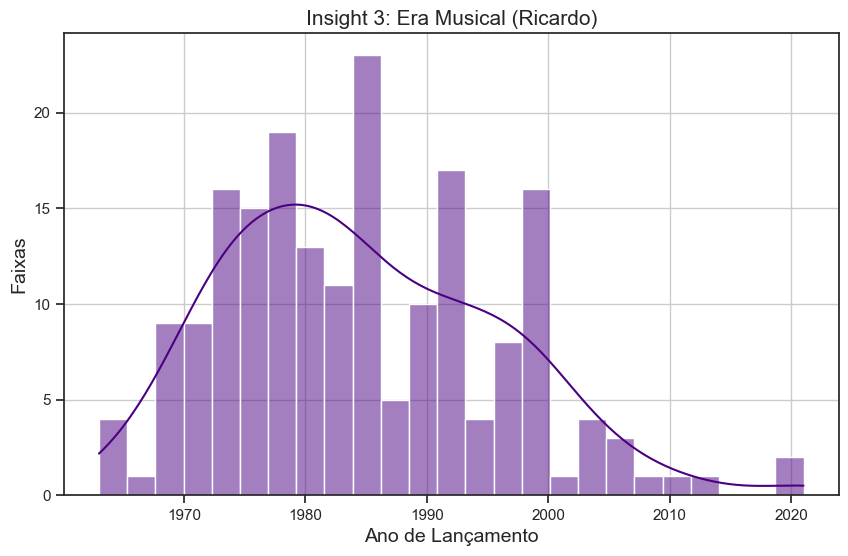
\includegraphics[width=0.78\textwidth]{ricardo_3_era.png}
\fontefig{Elaborado pelo autor (2026).}
\label{fig:ricardo-3}
\end{figure}

\begin{figure}[H]
\centering
\caption{Ricardo (input): concentração de artistas (Curva de Lorenz).}
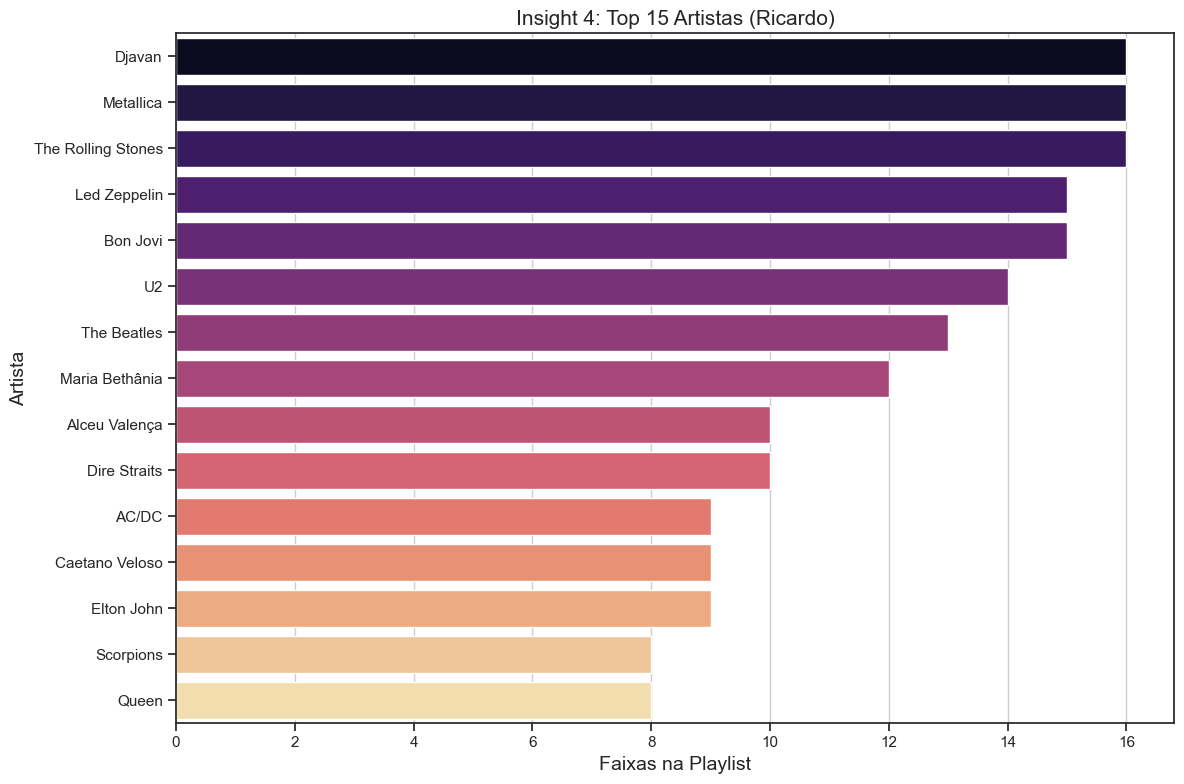
\includegraphics[width=0.78\textwidth]{ricardo_4_lorenz.png}
\fontefig{Elaborado pelo autor (2026).}
\label{fig:ricardo-4}
\end{figure}

\begin{figure}[H]
\centering
\caption{Ricardo (input): popularidade vs.\ alcance dos artistas.}
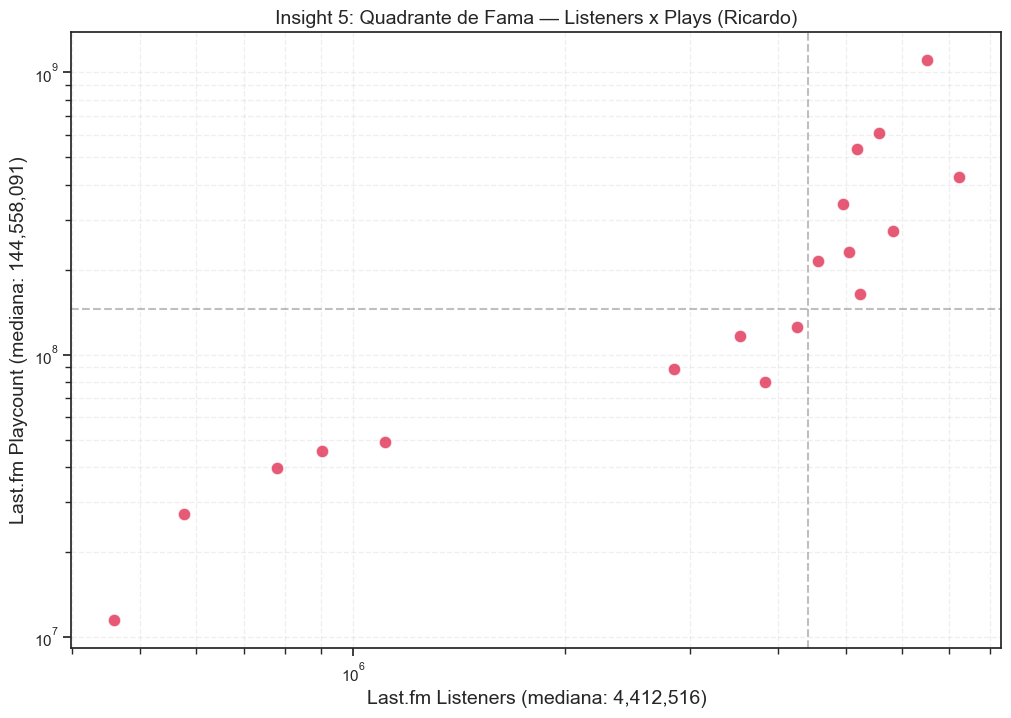
\includegraphics[width=0.85\textwidth]{ricardo_5_popfollow.png}
\fontefig{Elaborado pelo autor (2026).}
\label{fig:ricardo-5}
\end{figure}

\begin{figure}[H]
\centering
\caption{Ricardo (input): distribuição de duração das faixas.}
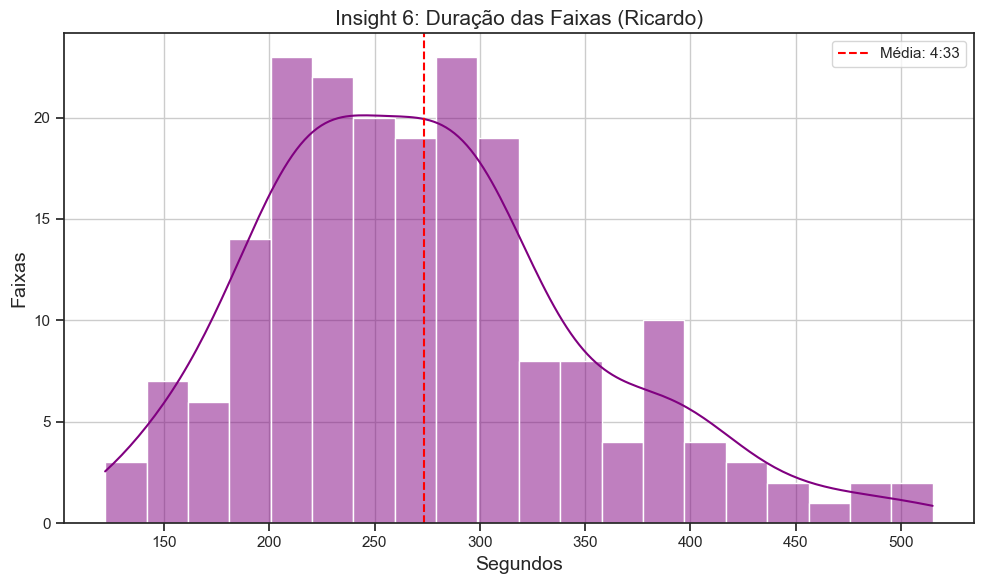
\includegraphics[width=0.78\textwidth]{ricardo_6_duracao.png}
\fontefig{Elaborado pelo autor (2026).}
\label{fig:ricardo-6}
\end{figure}

\section{Análise Comparativa e Validação dos Estímulos (Inputs)}

Para assegurar a integridade da auditoria, é imperativo validar se as personas
geradas representam, de fato, \emph{clusters} comportamentais distintos e
independentes. Esta etapa de \textbf{Validação Cruzada} (\emph{Cross-Validation})
tem como objetivo demonstrar a ortogonalidade dos vetores de entrada: comprovar
que os quatro perfis ocupam quadrantes separados no espaço vetorial de consumo,
minimizando o risco de contaminação cruzada no estágio inicial (\emph{Cold
Start}).

Esta validação estabelece a \textbf{Linha de Base} (\emph{Baseline}) do
experimento. A confirmação de que não há sobreposição significativa entre os
conjuntos de dados iniciais é pré-requisito para a inferência causal futura:
qualquer convergência (ou divergência) observada nas recomendações
(\emph{Outputs}), seja de conteúdo, de tema ou de magnitude de diversidade, 
poderá ser atribuída à interferência do algoritmo, e não à similaridade original
dos usuários.

\subsection{Métricas de Diversidade e Entropia da Informação}

A aplicação de indicadores de diversidade revela as diferenças estruturais na
``dieta informacional'' de cada persona. A Tabela~\ref{tab:diversidade} apresenta
a Entropia de Shannon (incerteza/variedade), a \textbf{\emph{Evenness} de Pielou}
($J = H/\log_2 S$, que normaliza a Shannon pelo seu teto teórico e isola a
\emph{uniformidade} da \emph{riqueza}; \citeonline{pielou1966measurement}), o
Coeficiente de Gini (desigualdade de atenção) e a Riqueza (artistas únicos, $S$).
Estas métricas dependem apenas da contagem de artistas únicos e suas
frequências, não foram afetadas pela transição de fonte e mantêm os valores
originalmente computados.

\begin{table}[H]
\centering
\caption{Métricas de diversidade dos inputs (Shannon, Pielou, Gini, riqueza).}
\label{tab:diversidade}
\footnotesize
\begin{tabularx}{\textwidth}{>{\bfseries\raggedright\arraybackslash}p{1.7cm} c c c c X}
\toprule
\textbf{Persona} & \textbf{Shannon} & \textbf{Pielou} & \textbf{Gini} & \textbf{Riqueza ($S$)} & \textbf{Interpretação Estrutural} \\
\midrule
Beatriz & 6,03 (Alta) & 0,92 & 0,42 (Média) & 94 & Consumo Exploratório/Caótico; ouvinte de \emph{hits}, alta rotatividade e baixa fidelidade a álbuns. \\
Daniel & 6,27 (Máxima) & 0,95 & 0,37 (Baixa) & 99 & Pulverização Funcional; foco na utilidade da ``faixa'', não na identidade do ``artista''. \\
Ricardo & 4,10 (Mínima) & \textbf{0,98} & 0,18 (Mínima) & 18 & Baixa riqueza, alta uniformidade; Shannon mínima decorre dos poucos artistas (18), não de concentração. \\
Sofia & 4,43 (Baixa) & 0,93 & 0,36 (Baixa) & 27 & Curadoria Seletiva; foco em \emph{Deep Cuts} de poucos artistas de nicho (escuta vertical). \\
\bottomrule
\end{tabularx}
\fontefig{Elaborado pelo autor (2026).}
\end{table}

\textbf{Análise.} O ponto decisivo é que a \emph{Evenness} de Pielou é alta e
praticamente plana (0,92--0,98) em todas as personas. Isso significa que as
grandes diferenças de Entropia de Shannon entre os perfis (4,10 a 6,27)
\textbf{não decorrem de diferenças de uniformidade, mas de diferenças de riqueza}
($S$): Ricardo tem Shannon baixa porque consome \emph{poucos} artistas (18), não
porque os distribui de forma desigual, ao contrário, sua distribuição é a mais
uniforme do estudo. Essa distinção entre riqueza e uniformidade é central para a
leitura correta do Capítulo~\ref{cap:resultados}, onde se demonstra que a
``convergência'' da Shannon nos \emph{outputs} é, na verdade, \textbf{expansão de
riqueza de catálogo} com a \emph{evenness} preservada, e não homogeneização de
entropia.

\subsection{Distribuição de Mercado (Cauda Longa)}

A análise da estratificação econômica dos artistas valida a hipótese de
polarização entre ``Cabeça'' (\emph{Head}) e ``Cauda'' (\emph{Tail}) da
distribuição de Pareto. Os limiares de classificação foram \textbf{calibrados por
discretização em percentis (\emph{quantile binning}) sobre um \emph{pool} único}
que combina os oito conjuntos do estudo
(quatro \emph{inputs} $+$ quatro \emph{outputs}, deduplicados por artista: 557
artistas), resultando em \textbf{P25 $=$ 65.376} e \textbf{P75 $=$ 474.962}
\emph{listeners} no Last.fm. O \emph{quantile binning} é um procedimento
não-paramétrico padrão para tornar estratos comparáveis entre amostras de escalas
distintas, sem impor um limiar absoluto arbitrário. Essa \textbf{régua única},
idêntica para
\emph{input} e \emph{output}, substitui os limiares absolutos baseados em
\emph{followers} do Spotify (deprecados em 02/2026) e torna os \emph{tiers}
diretamente comparáveis entre estímulo e recomendação; calibrá-los separadamente
por \emph{source} produziria classificações incomparáveis.

\begin{table}[H]
\centering
\caption{Distribuição de Cauda Longa dos inputs (régua única de \emph{listeners}).}
\label{tab:longtail}
\footnotesize
\begin{tabularx}{\textwidth}{>{\bfseries\raggedright\arraybackslash}p{1.6cm} >{\centering\arraybackslash}p{1.9cm} >{\centering\arraybackslash}p{1.9cm} >{\centering\arraybackslash}p{2.0cm} X}
\toprule
\textbf{Persona} & \textbf{\% \emph{Superstars} ($>$P75)} & \textbf{\% Médios (P25--P75)} & \textbf{\% Cauda Longa ($\leq$P25)} & \textbf{Perfil Econômico} \\
\midrule
Beatriz & 10,6\% & 75,5\% & 13,8\% & Consumidora de Massa; concentração em Médios brasileiros (sertanejo, funk). \\
Ricardo & \textbf{94,4\%} & 5,6\% & 0,0\% & Consumidor de Legado; foco quase exclusivo em gigantes consagrados. \\
Daniel & 5,1\% & 54,5\% & \textbf{40,4\%} & Consumidor Funcional Misto; fronteira entre \emph{bedroom producers} e produtores estabelecidos. \\
Sofia & 3,7\% & 40,7\% & \textbf{55,6\%} & Consumidora Subcultural; majoritariamente cauda longa, com poucas exceções consolidadas. \\
\bottomrule
\end{tabularx}
\fontefig{Elaborado pelo autor (2026).}
\end{table}

\textbf{Análise.} O contraste entre Ricardo (94,4\% \emph{Superstars}) e Sofia
(55,6\% Cauda Longa) cria o cenário ideal para auditar o viés econômico:
permitirá verificar se o algoritmo tenta forçar uma ``gentrificação'' do gosto de
Sofia, empurrando-a em direção à média de mercado para maximizar a retenção. O
uso de uma régua única (\emph{input} $+$ \emph{output}) também garante que
qualquer deslocamento de \emph{tier} observado no Capítulo~\ref{cap:resultados}
seja atribuível ao algoritmo, e não a uma diferença de calibração entre os
conjuntos.

\subsection{Análise Visual Cruzada e Topologia dos Dados}

As visualizações a seguir sintetizam graficamente as diferenças estruturais entre
as quatro personas, comprovando a heterogeneidade da amostra inicial através de
uma análise topológica dos dados. O objetivo destas representações é demonstrar a
\textbf{ortogonalidade dos perfis}: cada persona ocupa uma região distinta no
espaço vetorial de consumo.

\textbf{A) Matriz de Similaridade (Índice de Jaccard).} Esta matriz atua como a
prova definitiva do isolamento experimental. A predominância absoluta de valores
nulos (0,00) ou próximos a zero nas interseções entre personas confirma que não
há compartilhamento de repertório, garantindo que o estado de \emph{Cold Start} é
único para cada agente.

\begin{figure}[H]
\centering
\caption{Matriz de Similaridade (Índice de Jaccard) entre as personas (input).}
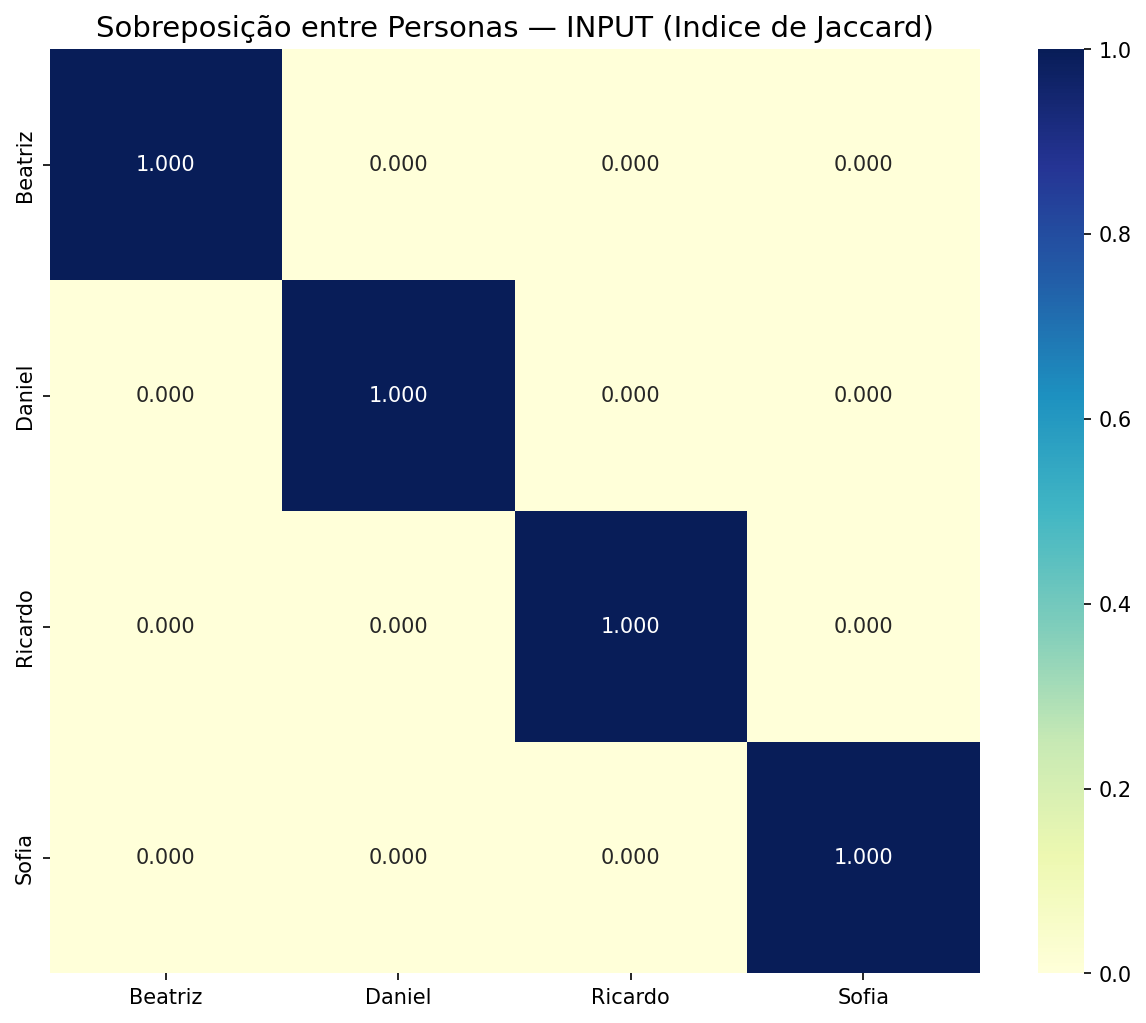
\includegraphics[width=0.72\textwidth]{cross_jaccard.png}
\fontefig{Elaborado pelo autor (2026).}
\label{fig:cross-jaccard}
\end{figure}

\textbf{B) Mapeamento da Economia da Atenção (\emph{Scatter Plot}:
Ouvintes $\times$ Execuções históricas).} Este gráfico espacializa a Teoria da
Cauda Longa (\emph{The Long Tail}), cruzando o número de \emph{listeners} únicos
e o \emph{playcount} histórico dos artistas (Last.fm), que substituem a
popularidade e os seguidores do Spotify após a migração descrita na
Seção~\ref{sec:adaptacao}. O Quadrante Superior Direito (\emph{Head}) é
ocupado por Ricardo e Beatriz, representando o consumo de alta visibilidade e
capital social; o Quadrante Inferior Esquerdo (\emph{Tail}), por Sofia e Daniel,
representando a zona de obscuridade e nicho. A clara separação visual valida a
capacidade do experimento de auditar o viés algorítmico em diferentes estratos de
poder econômico.

\begin{figure}[H]
\centering
\caption{Mapeamento da Economia da Atenção: popularidade vs.\ alcance, por persona (input).}
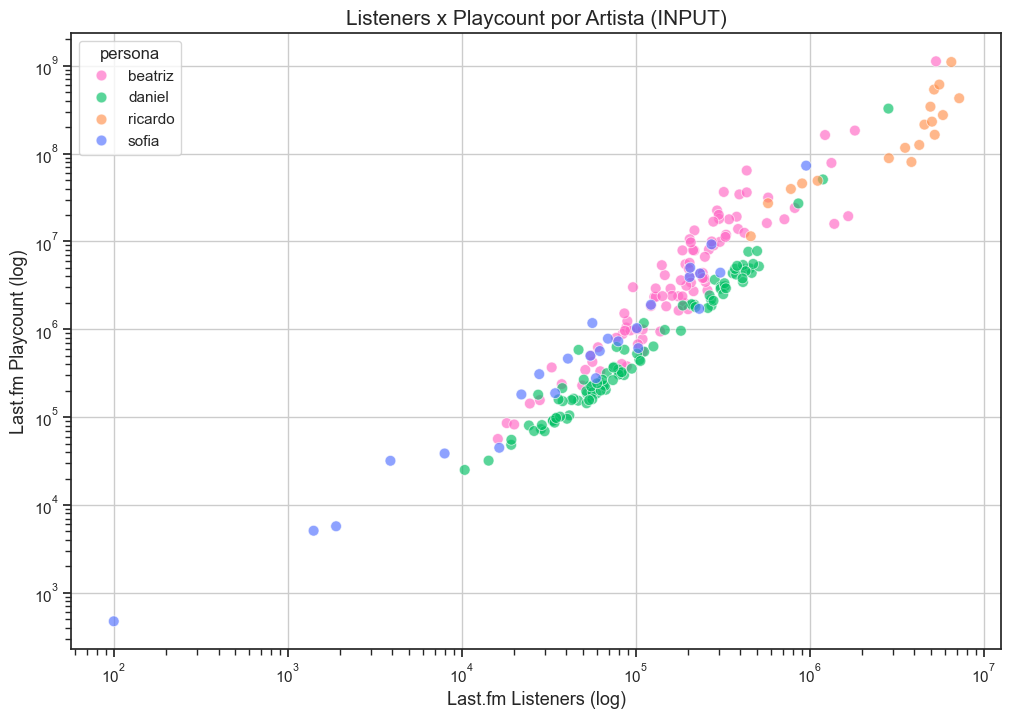
\includegraphics[width=0.85\textwidth]{cross_popfollow.png}
\fontefig{Elaborado pelo autor (2026).}
\label{fig:cross-popfollow}
\end{figure}

\textbf{C) Cronologia do Consumo (Distribuição Temporal).} A visualização de
densidade temporal (\emph{KDE Plot}) valida o controle da variável ``Tempo''.
Observa-se a sobreposição das curvas de Daniel, Beatriz e Sofia na extrema
direita (anos 2020), enquanto a curva de Ricardo se isola à esquerda (século XX).
Este gráfico serve como linha de base para medir o \textbf{Viés de Recência}:
deslocamentos futuros da curva de Ricardo para a direita indicarão uma tentativa
do sistema de impor novidades a um perfil conservador.

\begin{figure}[H]
\centering
\caption{Cronologia do consumo: distribuição temporal das faixas por persona (KDE, input).}
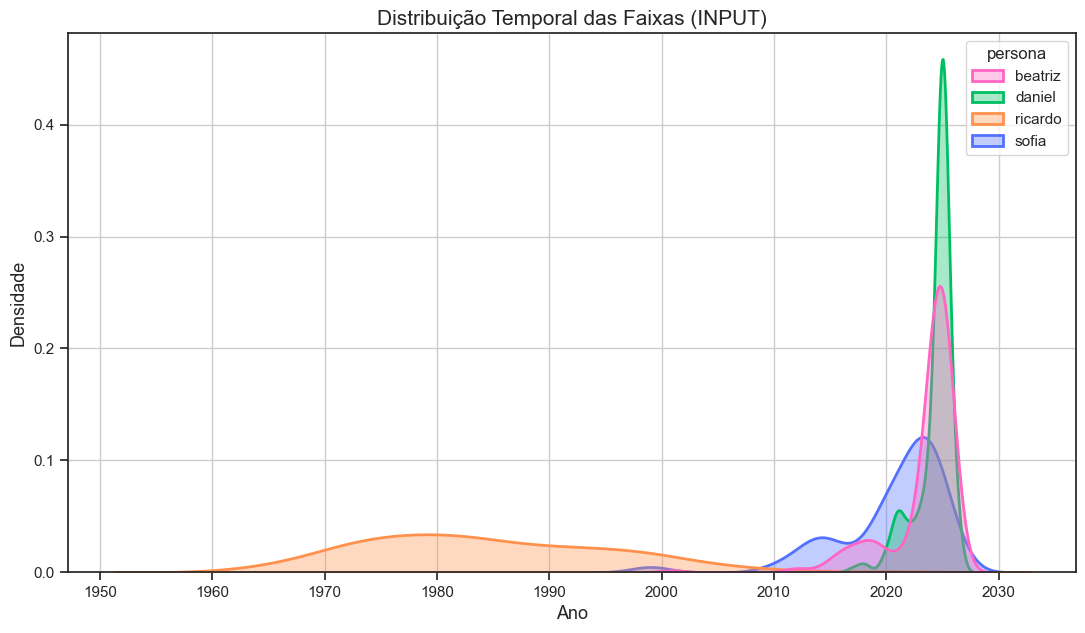
\includegraphics[width=0.85\textwidth]{cross_era.png}
\fontefig{Elaborado pelo autor (2026).}
\label{fig:cross-era}
\end{figure}

\textbf{D) Curva de Lorenz (Concentração de Artistas).} O gráfico ilustra a
desigualdade na distribuição de atenção. A curva de Ricardo (mais distante da
diagonal perfeita) confirma visualmente sua fidelidade monástica a poucos
artistas, enquanto a curva de Beatriz (mais próxima da diagonal) demonstra um
consumo pulverizado. Essa métrica será essencial para auditar se o algoritmo
respeita a profundidade de catálogo ou se tende a fragmentar a experiência de
escuta.

\begin{figure}[H]
\centering
\caption{Concentração de artistas: Curva de Lorenz comparada entre personas (input).}
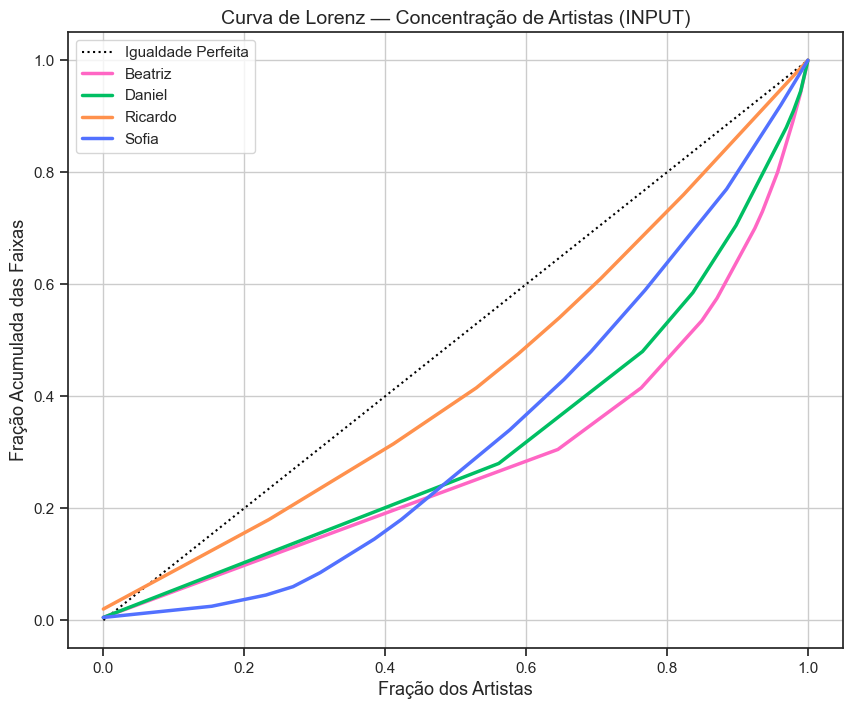
\includegraphics[width=0.85\textwidth]{cross_lorenz.png}
\fontefig{Elaborado pelo autor (2026).}
\label{fig:cross-lorenz}
\end{figure}

\section{Síntese Metodológica e Limitações}
\label{sec:limitacoes}

A estrutura metodológica aqui apresentada estabelece um ambiente controlado e
auditável para a investigação dos algoritmos de recomendação. A validação
estatística dos \emph{inputs} confirma que as quatro personas sintéticas, 
Beatriz, Daniel, Sofia e Ricardo, constituem instrumentos de medição
calibrados, representando vetores de comportamento distintos e isolados.

As métricas de diversidade (Shannon), desigualdade (Gini) e similaridade
(Jaccard) calculadas nesta etapa formam a \textbf{Linha de Base (Baseline)} do
estudo. Nos capítulos subsequentes, esses mesmos indicadores serão reaplicados
sobre as listas de recomendação geradas pelo Spotify (\emph{Daily Mix 1--6}),
permitindo a comparação \emph{Input vs. Output}.

A comparação direta entre os valores de \emph{Input} (apresentados neste
capítulo) e os valores de \emph{Output} (a serem analisados no
Capítulo~\ref{cap:resultados}) revela o ``Delta Algorítmico'': a magnitude e a
direção da interferência do sistema sobre o gosto do usuário. Dessa forma, será
possível responder aos objetivos da pesquisa, determinando se a plataforma atua
como um espelho fiel das preferências do usuário ou como um prisma que distorce a
diversidade cultural em favor de padrões comerciais hegemônicos.

\subsection{Limitações Metodológicas e Achado Original}

\textbf{A) Pré-requisito não-trivial de Incubação Algorítmica.} Verificou-se
empiricamente que o sistema do Spotify \textbf{não materializa as \emph{playlists}
personalizadas} (\emph{Daily Mix}, \emph{Discover Weekly}, \emph{Release Radar})
apenas com base em \emph{likes} e \emph{follows} declarados pelo usuário. A
geração desses produtos exige um histórico mínimo de \textbf{escuta efetiva},
funcionando como sinal implícito de validação. Para satisfazer este
pré-requisito, conduziu-se aproximadamente \textbf{40 horas de escuta no modo
``Aleatório Inteligente'' (\emph{Smart Shuffle})} por conta-persona, 
totalizando $\sim$160 horas de incubação somadas. A escolha do \emph{Smart
Shuffle} (em detrimento do \emph{shuffle} puro) é deliberada: este modo intercala
faixas curtidas com sugestões algorítmicas, garantindo registro de interação
tanto com o \emph{input} declarado (\emph{likes}) quanto com recomendações
exploratórias. Este pré-requisito constitui uma \textbf{observação metodológica
original} desta pesquisa, raramente documentada na literatura de auditoria
algorítmica musical. Estudos futuros que tentem replicar este \emph{pipeline} sem
a etapa de incubação ativa \textbf{não conseguirão coletar os \emph{outputs}
algorítmicos}.

\textbf{B) Achado Central, Obstrução Progressiva da API como Meta-Evidência.}
O acesso à Spotify Web API foi progressivamente restringido em \textbf{três
ondas parcialmente não-anunciadas} entre o final de 2024 e o primeiro semestre
de 2026 (detalhadas na Seção~\ref{sec:adaptacao}). A primeira antecede a fase de
coleta; as duas seguintes foram \textbf{testemunhadas durante a execução} do
experimento: a Onda 1 (Nov/2024, anterior à coleta)
removeu o acesso a \emph{playlists} algorítmicas para \emph{apps} em modo
\emph{development}; a Onda 2 (Fev/2026, durante a pesquisa) exigiu \emph{Premium}
para o titular do
\emph{app}, limitou a 5 usuários autorizados, depreciou o \emph{endpoint}
\texttt{/playlists/\{id\}/tracks} e restringiu \texttt{/items} a apenas dono ou
colaborador; e a Onda 3 (abr/2026, identificação empírica, sem \emph{changelog}
público) removeu
sistematicamente os campos \texttt{popularity}, \texttt{followers} e
\texttt{genres}. A natureza progressiva, parcialmente não-anunciada e unilateral
dessas restrições \textbf{constitui em si um achado científico relevante}: ela
ilustra empiricamente o argumento central da Introdução sobre a \textbf{opacidade
e a governança algorítmica} das plataformas de \emph{streaming}, pois, no caso
das duas ondas de 2026, o próprio
instrumental técnico necessário à auditoria foi sendo obstruído \emph{durante} a
execução do experimento, e não apenas antes dele. Esta observação configura-se como \textbf{meta-evidência}
da assimetria informacional entre plataformas e atores externos, alinhando-se ao
método etnográfico-experimental de \citeonline{eriksson2019spotify} em
\emph{Spotify Teardown}, que já denunciava a resistência da plataforma ao
escrutínio independente.

\textbf{C) Resposta Metodológica, \emph{Apples-to-Apples} via Fontes Externas.}
Para preservar o rigor e a comparabilidade \emph{Input vs. Output}, adotou-se a
substituição das métricas comprometidas por dados de \textbf{fontes externas
consagradas} (Last.fm $+$ MusicBrainz), aplicadas consistentemente aos dois lados
da auditoria. Esta solução transforma a limitação em oportunidade, a pesquisa
passa a se ancorar em três bases de dados independentes (Spotify para
\emph{tracks}/álbuns/datas; Last.fm para audiência/gêneros; MusicBrainz para
\emph{life-span}/tipo/região), aumentando a triangulação metodológica.

\textbf{D) Outras Limitações.}
\begin{itemize}
  \item \textbf{Cobertura do MusicBrainz para \emph{bedroom producers}:} a
  análise de \emph{life-span} (\texttt{mb\_career\_start}) cobre 100\% dos
  artistas de Ricardo, mas apenas 20\% dos de Daniel, refletindo a invisibilidade
  de produtores \emph{lo-fi} obscuros nos catálogos institucionais.
  \item \textbf{Viés geocultural do Last.fm:} as bases Last.fm e MusicBrainz
  subcontam artistas brasileiros (sertanejo, funk, indie nacional) frente ao
  repertório anglófono global. Isso se manifesta nos dados: a cobertura
  simultânea cai para 86,7\% em Sofia, e a composição por país
  (\texttt{mb\_country}) varia de 0\% de artistas BR em Daniel a 61,8\% em Beatriz
  no \emph{input}. A consequência é que os \emph{listeners}/\emph{tiers} de
  artistas brasileiros podem estar subestimados por \emph{artefato de cobertura};
  por isso, os deltas \emph{within-persona} são mais defensáveis do que as
  comparações \emph{cross-persona} de magnitude absoluta.
  \item \textbf{Heterogeneidade da fonte de \emph{tags} (HHI):} o HHI é calculado
  sobre a melhor fonte de \emph{tags} por faixa, na ordem \texttt{mb\_tags} $>$
  \texttt{lastfm\_tags} $>$ \texttt{artist\_genres}. A mistura de granularidades
  introduz ruído menor, reforçando a leitura \textbf{relativa} do HHI.
  \item \textbf{Generalização limitada:} os resultados refletem o comportamento
  do algoritmo do Spotify para perfis brasileiros configurados em abril de 2026;
  extensões para outros mercados ou momentos exigem replicação independente.
  \item \textbf{Possível variabilidade temporal:} os \emph{Daily Mixes} são
  atualizados continuamente. A coleta foi feita em janela curta (mesma semana de
  28/04/2026) para minimizar variabilidade.
\end{itemize}

% ==========================================================
\chapter{Resultados: Análise dos Outputs e o Delta Algorítmico}
\label{cap:resultados}
% ==========================================================

Concluída a fase de validação dos \emph{inputs}
(Capítulo~\ref{cap:metodologia}), o presente capítulo apresenta a análise
empírica dos \emph{outputs} algorítmicos coletados, as faixas que o Spotify
recomendou aos quatro perfis sintéticos por meio dos \emph{Daily Mixes}, após o
período de incubação descrito na Seção~\ref{sec:limitacoes}. O objetivo central
deste capítulo é responder à pergunta condutora da pesquisa: \textbf{em que
magnitude e direção o algoritmo de recomendação distorce o perfil declarado de
cada usuário?}

A análise é estruturada em quatro etapas: (i) apresentação descritiva dos
\emph{outputs} coletados; (ii) cálculo da Taxa de \emph{Overlap} Interno
(redundância dentro da bolha de cada persona); (iii) análise do Delta Algorítmico,
comparação direta \emph{Input vs. Output} das treze métricas centrais; e (iv)
síntese e teste das quatro hipóteses formuladas por persona no
Capítulo~\ref{cap:metodologia}.

\section{Apresentação dos Outputs Coletados (Daily Mixes)}

Após o período de incubação algorítmica ($\sim$40 horas de escuta efetiva por
persona, em modo \emph{Smart Shuffle}), o sistema do Spotify gerou seis
\emph{Daily Mixes} para cada conta. Estas \emph{playlists} foram copiadas
manualmente para \emph{playlists} espelho de propriedade de cada persona, 
\emph{workaround} necessário em virtude da Onda 1 de restrição da API
(Seção~\ref{sec:adaptacao}). Durante o procedimento de cópia, faixas duplicadas
entre os seis \emph{mixes} foram automaticamente filtradas pelo próprio cliente
do Spotify, gerando o conjunto final consolidado. A Tabela~\ref{tab:volume}
sintetiza o volume de dados coletados.

\begin{table}[H]
\centering
\caption{Volume e cobertura dos Outputs.}
\label{tab:volume}
\footnotesize
\begin{tabularx}{\textwidth}{l *{5}{>{\centering\arraybackslash}X}}
\toprule
\textbf{Persona} & \textbf{Faixas únicas (Output)} & \textbf{Faixas (Input)} & \textbf{$\Delta$ tamanho} & \textbf{Artistas únicos (Output)} & \textbf{Cobertura ambas as fontes} \\
\midrule
Beatriz & 276 & 200 & $+38{,}0\%$ & 121 & 100,0\% \\
Daniel  & 281 & 200 & $+40{,}5\%$ & 115 & 98,6\% \\
Ricardo & 268 & 200 & $+34{,}0\%$ & 126 & 100,0\% \\
Sofia   & 264 & 200 & $+32{,}0\%$ & 90  & 86,7\% \\
\bottomrule
\end{tabularx}
\fontefig{Elaborado pelo autor (2026).}
\end{table}

\textbf{Observação.} O tamanho dos \emph{outputs} é sistematicamente maior que o
dos \emph{inputs} (200 faixas), efeito direto dos seis \emph{Daily Mixes}
contendo aproximadamente 50 faixas cada ($\sim$300 faixas brutas, das quais
6--12\% são duplicatas removidas). 100\% das faixas obtiveram ao menos dados do
Last.fm; a coluna de cobertura reporta a presença \emph{simultânea} das duas
fontes. A cobertura mais baixa de Sofia (86,7\%) reflete a menor presença de
artistas \emph{underground} no MusicBrainz.

\section{Taxa de Overlap Interno: Redundância Intra-Persona}

Esta métrica original do estudo quantifica quanto o algoritmo ``insiste nas
mesmas faixas'' entre os seis \emph{clusters} (\emph{Daily Mixes}) gerados para
uma mesma persona. Operacionalmente, é calculada como:
\[ \text{Overlap Interno} = \frac{300 - N}{300} \]
onde $N$ é o número de faixas únicas após \emph{dedupe} (e 300 representa o
\emph{pool} bruto estimado de seis \emph{mixes} $\times$ 50 faixas). Quanto maior
a taxa, mais redundante é o conjunto de \emph{clusters}.

\begin{table}[H]
\centering
\caption{Taxa de Overlap Interno entre os Daily Mixes.}
\label{tab:overlap}
\footnotesize
\begin{tabularx}{\textwidth}{>{\bfseries\raggedright\arraybackslash}p{1.7cm} c c c X}
\toprule
\textbf{Persona} & \textbf{Faixas únicas ($N$)} & \textbf{Duplicatas} & \textbf{Taxa de Overlap Interno} & \textbf{Interpretação} \\
\midrule
Daniel  & 281 & 19 & \textbf{6,33\%}  & Variedade alta dentro do nicho \emph{lo-fi} (muito material disponível). \\
Beatriz & 276 & 24 & 8,00\%  & Variedade moderada (catálogo brasileiro \emph{mainstream} amplo). \\
Ricardo & 268 & 32 & 10,67\% & Redundância média (catálogo clássico tem repertório finito de ``lendas''). \\
Sofia   & 264 & 36 & \textbf{12,00\%} & Maior redundância, bolha mais estreita. \\
\bottomrule
\end{tabularx}
\fontefig{Elaborado pelo autor (2026).}
\end{table}

\textbf{Indicador exploratório (com ressalvas).} O perfil Sofia apresenta a maior
taxa de redundância entre as quatro personas, sugerindo que, com menos
diversidade no \emph{input} declarado (27 artistas únicos contra 99 de Daniel), o
algoritmo tende a repetir faixas entre \emph{clusters}. Esta leitura deve ser
tomada como \textbf{indicador exploratório, e não como achado consolidado}, por
duas limitações estruturais: (i) a métrica é uma transformação determinística e
decrescente do número de faixas únicas, fixado o \emph{pool} em 300,
$(300-N)/300$ não acrescenta informação independente do próprio $N$; e (ii) a
deduplicação entre os seis \emph{Daily Mixes} foi feita automaticamente pelo
cliente do Spotify \emph{antes} da contagem, de modo que o valor bruto do
\emph{pool} é uma suposição não verificável. A amplitude observada é estreita
(6,33\% a 12,00\%); evita-se, portanto, qualquer leitura causal forte de ``bolha
de filtro'' a partir deste indicador, reservando-se a evidência de estreitamento
às métricas de Jaccard \emph{cross-persona} (Seção~\ref{sec:diversidade-output}).

\section{O Delta Algorítmico: Visão Geral}

O \emph{Delta Algorítmico} é o resultado quantitativo central deste estudo: a
diferença entre o valor de cada métrica no \emph{Output} (recomendações
algorítmicas) e no \emph{Input} (perfil declarado pelo usuário), expresso em
variação percentual. A Figura~\ref{fig:heatmap} condensa os deltas de
\textbf{treze métricas $\times$ quatro personas} em uma única visualização.

\begin{figure}[H]
\centering
\caption{Heatmap do Delta Algorítmico Percentual.}
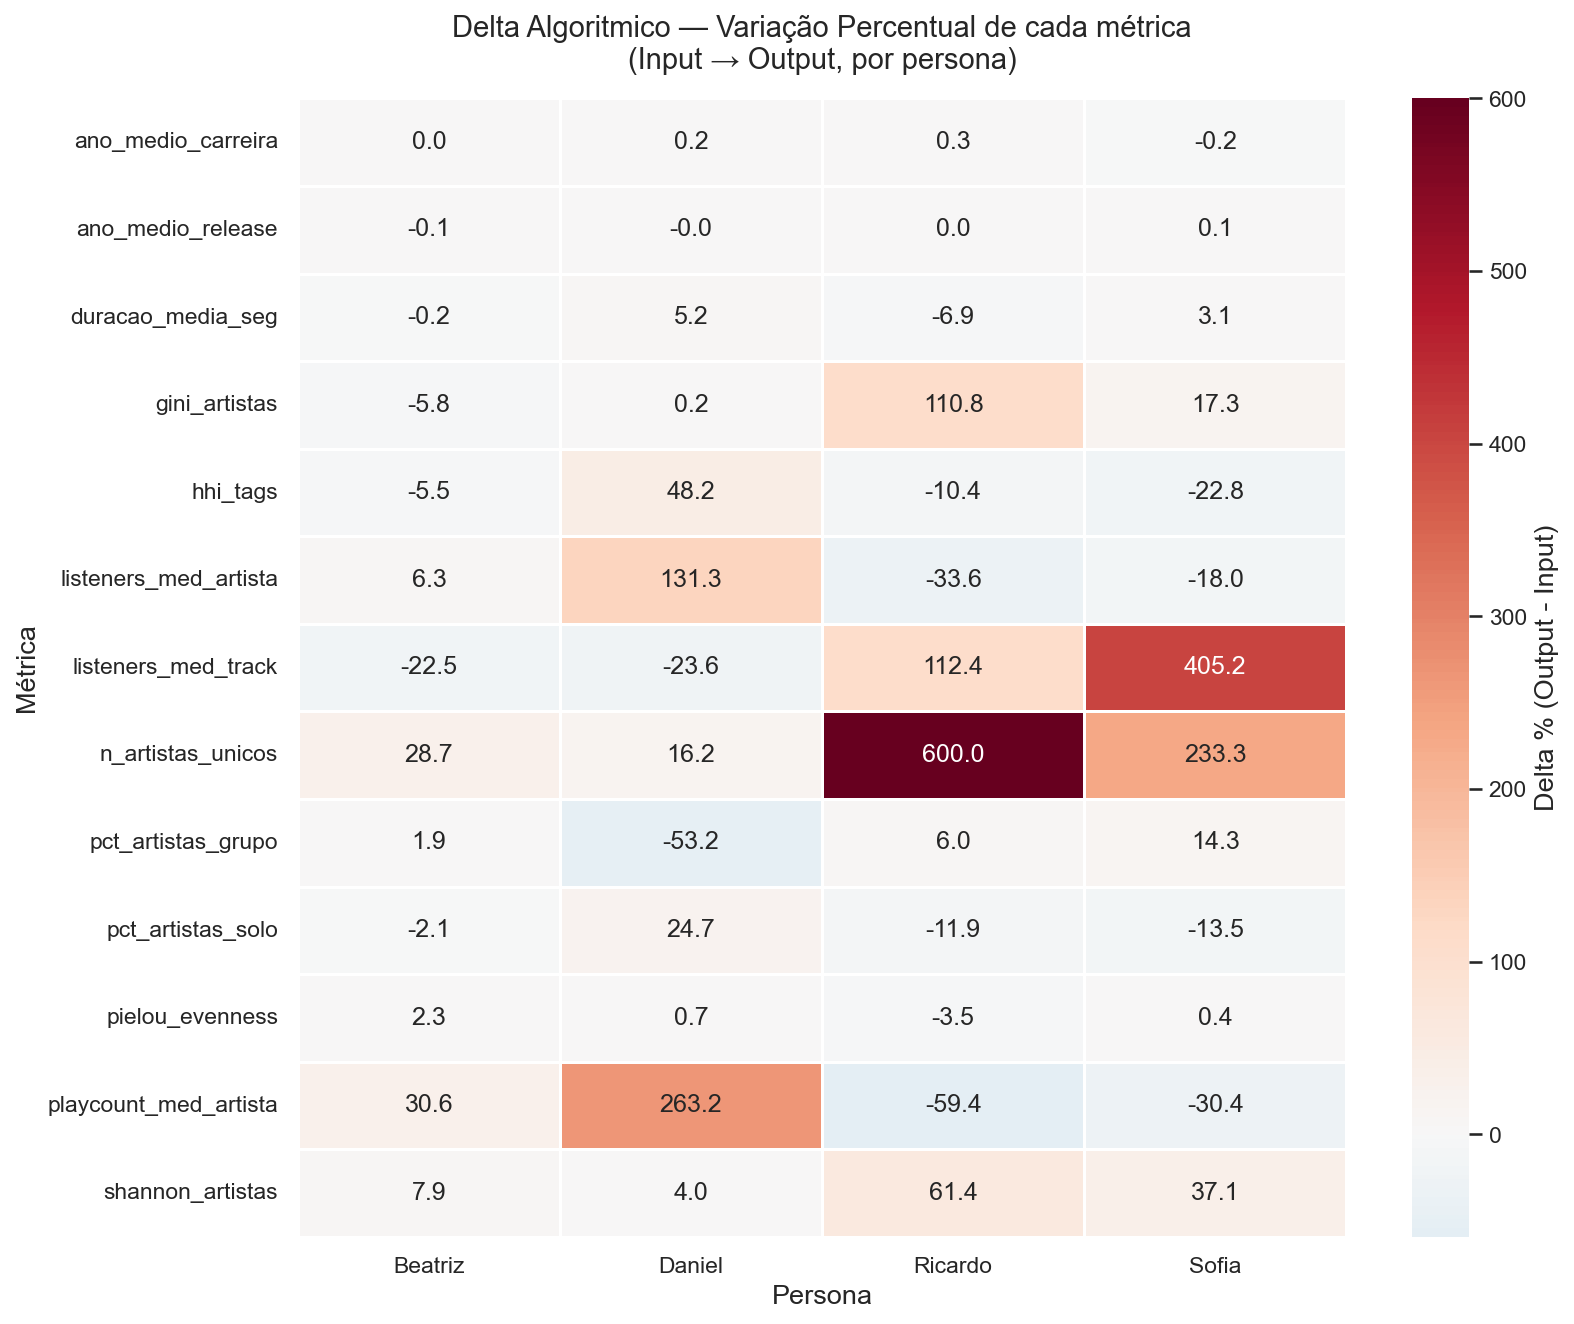
\includegraphics[width=0.95\textwidth]{cmp_heatmap_delta.png}
\fontefig{Elaborado pelo autor (2026).}
\label{fig:heatmap}
\end{figure}

\noindent Cores em vermelho indicam crescimento da métrica do \emph{input} para o
\emph{output}; cores em azul indicam queda. Quanto mais saturada, maior a
magnitude da variação. A Tabela~\ref{tab:delta} sintetiza os deltas percentuais.

\begin{table}[H]
\centering
\caption{Delta Algorítmico Percentual (Input $\rightarrow$ Output).}
\label{tab:delta}
\footnotesize
\begin{tabular}{>{\raggedright\arraybackslash}p{5.5cm} c c c c}
\toprule
\textbf{Métrica} & \textbf{Beatriz} & \textbf{Daniel} & \textbf{Ricardo} & \textbf{Sofia} \\
\midrule
Shannon (Artistas)            & $+7{,}9\%$  & $+4{,}0\%$            & $\mathbf{+61{,}4\%}$  & $\mathbf{+37{,}1\%}$ \\
Gini (Artistas)               & $-5{,}8\%$  & $+0{,}2\%$            & $\mathbf{+110{,}8\%}$ & $+17{,}3\%$ \\
HHI (Tags)                    & $-5{,}5\%$  & $\mathbf{+48{,}2\%}$  & $-10{,}5\%$           & $-22{,}8\%$ \\
Listeners Mediano (Artista)   & $+6{,}3\%$  & $\mathbf{+131{,}3\%}$ & $-33{,}6\%$           & $-18{,}0\%$ \\
Playcount Mediano (Artista)   & $+30{,}6\%$ & $\mathbf{+263{,}2\%}$ & $-59{,}4\%$           & $-30{,}4\%$ \\
Listeners Mediano (Track)     & $-22{,}5\%$ & $-23{,}6\%$           & $+112{,}4\%$         & $\mathbf{+405{,}2\%}$ \\
n.\ Artistas Únicos           & $+28{,}7\%$ & $+16{,}2\%$           & $\mathbf{+600{,}0\%}$ & $+233{,}3\%$ \\
\% Artistas Solo (Person)     & $-2{,}1\%$  & $\mathbf{+24{,}7\%}$  & $-11{,}9\%$           & $-13{,}5\%$ \\
\% Artistas Grupo (Group)     & $+1{,}9\%$  & $\mathbf{-53{,}2\%}$  & $+6{,}0\%$           & $+14{,}3\%$ \\
Ano Médio (Carreira)          & $+0{,}0\%$  & $+0{,}2\%$            & $+0{,}3\%$           & $-0{,}2\%$ \\
Ano Médio (Release)           & $-0{,}1\%$  & $-0{,}0\%$            & $+0{,}0\%$           & $+0{,}1\%$ \\
Duração Média                 & $-0{,}2\%$  & $+5{,}2\%$            & $-6{,}9\%$           & $+3{,}1\%$ \\
\bottomrule
\end{tabular}
\fontefig{Elaborado pelo autor (2026).}
\end{table}

A leitura horizontal (por métrica) revela quais aspectos do consumo o algoritmo
mais distorce; a leitura vertical (por persona) mostra quais perfis sofrem maior
interferência.

\textbf{Nota sobre incerteza (tratamento inferencial, Seção~\ref{sec:inferencial}).}
Cada delta ``manchete'' deste capítulo é acompanhado de sua medida de incerteza,
computada pela rotina de inferência estatística descrita na
Seção~\ref{sec:inferencial}. Para as medianas de audiência,
reportam-se intervalos de confiança de 95\% por \emph{bootstrap} e, quando se
comparam distribuições \emph{track-level}, o $p$-valor de Mann-Whitney U. Por
exemplo: Daniel, \emph{listeners}/artista $79.595 \rightarrow 184.082$
($\mathbf{+131{,}3\%}$), IC95\% \emph{input} [64.290; 111.322] vs.\ \emph{output}
[146.972; 221.535], sem sobreposição; Sofia, \emph{listeners}/\emph{track}
$1.223 \rightarrow 6.178$ ($\mathbf{+405{,}2\%}$), Mann-Whitney
$p \approx 1{,}3 \times 10^{-16}$; Ricardo, \emph{listeners}/\emph{track}
$311.105 \rightarrow 660.893$ ($\mathbf{+112\%}$), $p \approx 2{,}1 \times
10^{-7}$. As variações de riqueza (ex.: Ricardo $+600\%$) são qualificadas pela
rarefação (Seção~\ref{sec:diversidade-output}).

\textbf{Achado preliminar (visão geral).} A magnitude da distorção \textbf{cresce
em ordem inversa ao alinhamento do perfil com o \emph{mainstream}}. Beatriz
(controle \emph{mainstream}) mostra apenas mudanças tímidas; Daniel (funcional,
mas comoditizado) mostra distorções moderadas; Sofia e Ricardo (perfis verticais
e desviantes do \emph{mainstream}) sofrem distorções extremas em múltiplas
dimensões.

\noindent\textbf{Guia de leitura das figuras comparativas (Figuras 4.2 a 4.7).}
As figuras que acompanham a análise persona a persona (Seção 4.4)
são todas \textbf{cross-persona}: cada uma apresenta as quatro personas lado a
lado (barras ou curvas \emph{input} vs.\ \emph{output}), e não apenas o perfil da
subseção em que aparece. Elas são posicionadas junto da persona que melhor
ilustram --- a Figura~\ref{fig:bar-listeners} (audiência) junto de Daniel, a
Figura~\ref{fig:tags} (\emph{tags}) junto de Ricardo, e assim por diante ---, mas
devem ser lidas \textbf{comparativamente}: a coluna ou curva de cada persona só
ganha sentido no contraste com as demais. O leitor pode, portanto, retornar a
qualquer uma delas ao acompanhar qualquer persona. Este bloco funciona como um
\textbf{painel comparativo único}, distribuído pelo capítulo por proximidade
temática, e não como gráficos isolados de cada perfil.

\section{Análise Persona por Persona}

\subsection{Beatriz (Mainstream): O Grupo de Controle Validado}

A persona Beatriz, projetada como controle \emph{mainstream} brasileiro, exibe os
menores deltas entre as quatro personas. As métricas críticas variam dentro de
margens estreitas: Shannon \emph{entropy} $+7{,}9\%$, \emph{listeners} por artista
$+6{,}3\%$, percentuais de tipo de artista praticamente inalterados (variação
$<$3\%). A Figura~\ref{fig:kde-listeners} (KDE de \emph{listeners} por artista)
mostra que as duas distribuições, \emph{input} e \emph{output}, quase se
sobrepõem para Beatriz, com leve deslocamento à direita no \emph{output}.

\begin{figure}[H]
\centering
\caption{Distribuição de \emph{Listeners} por Artista (Last.fm), em escala logarítmica, \emph{Input} vs.\ \emph{Output}.}
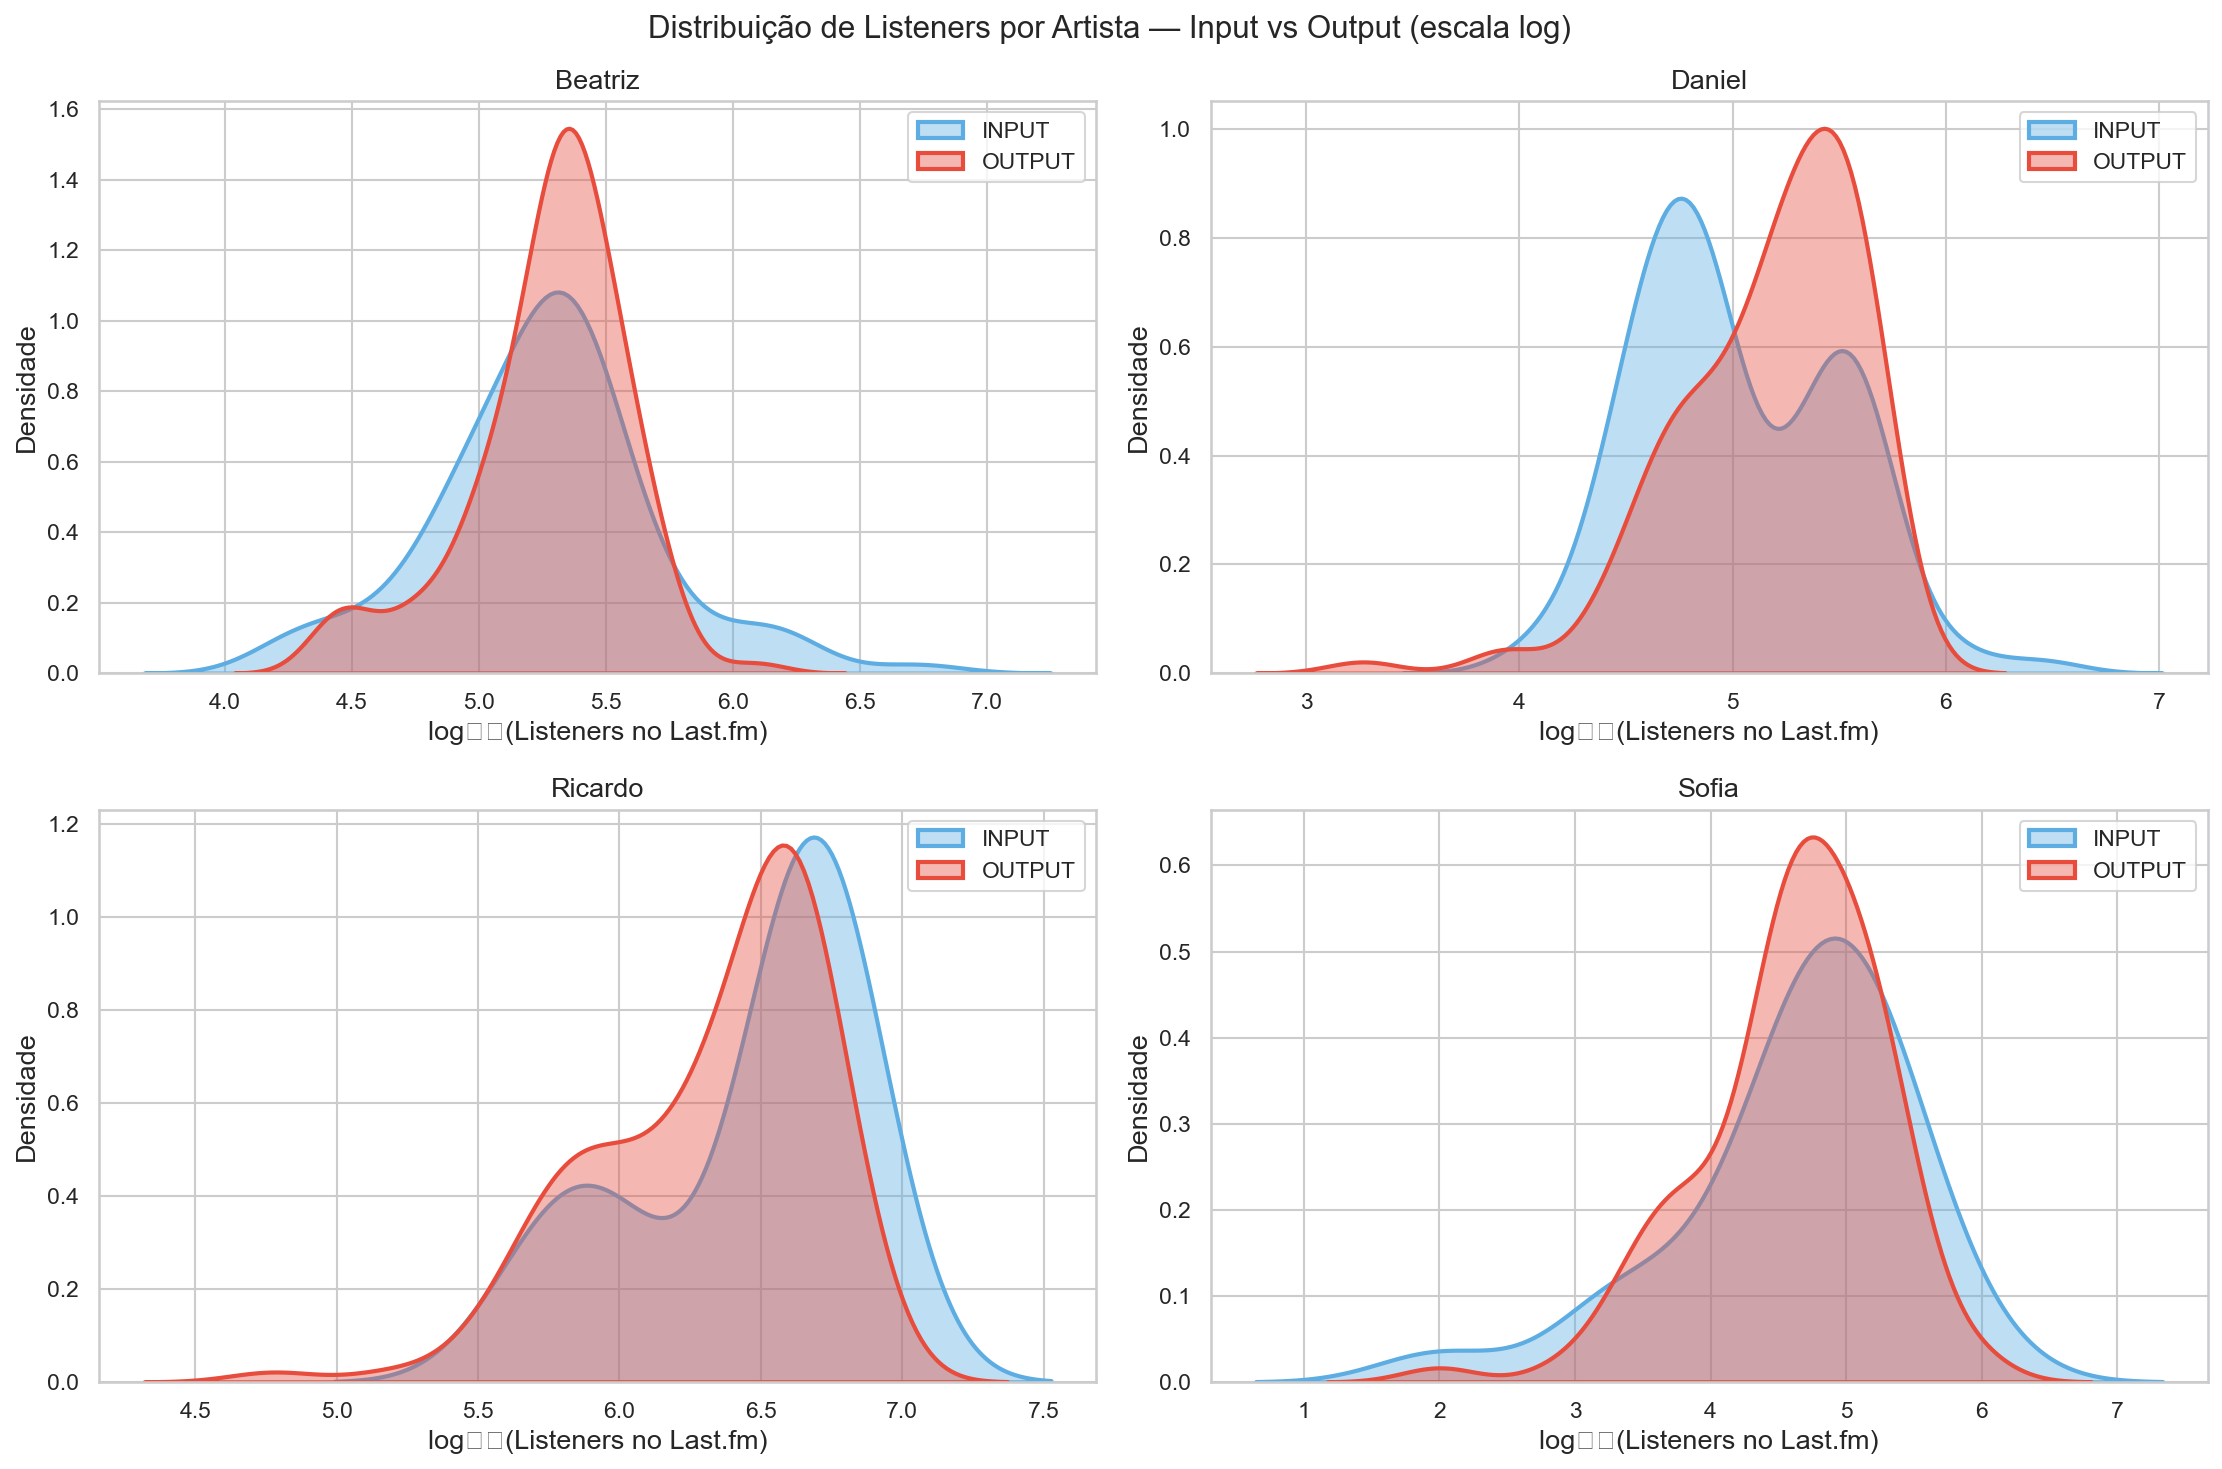
\includegraphics[width=0.95\textwidth]{cmp_kde_listeners.png}
\fontefig{Elaborado pelo autor (2026).}
\label{fig:kde-listeners}
\end{figure}

\noindent Beatriz: distribuições quase coincidentes; Daniel: deslocamento à
direita expressivo (efeito \emph{mainstream}); Ricardo: deslocamento à esquerda
(algoritmo encontra artistas menos consagrados); Sofia: deslocamento bimodal
sutil.

A leve elevação do \texttt{playcount\_med\_artista} ($+30{,}6\%$) e dos
\emph{listeners} ($+6{,}3\%$) indica que o algoritmo \textbf{adiciona artistas com
performance histórica ainda maior}, sem alterar a estrutura geral do perfil. Em
termos de \emph{tags}, observa-se manutenção da concentração temática (sertanejo,
brazil, pop). A composição solo/grupo mantém o equilíbrio do \emph{input}
($\sim$60/40).

\textbf{Conclusão para Beatriz.} O algoritmo ``comportou-se bem'', não há
distorção significativa do perfil declarado. Esta conclusão é metodologicamente
importante: valida o instrumental de medição. Caso Beatriz também apresentasse
grandes deltas, seria difícil isolar viés algorítmico de ruído experimental. A
baixa interferência sobre o perfil \emph{mainstream} \textbf{reforça a
confiabilidade dos achados nas demais personas}, onde os deltas são marcadamente
maiores.

\subsection{Daniel (Lo-fi): Confirmação do Viés de Popularidade}

A persona Daniel, projetada como consumidor funcional de \emph{lo-fi beats}
(perfil de Cauda Longa funcional), revela o achado mais nítido sobre \textbf{viés
de popularidade}. Os \emph{listeners} medianos por artista saltam de
\textbf{79.595 para 184.082 ($+131{,}3\%$)}, e o \emph{playcount} mediano salta de
\textbf{348.630 para 1.266.167 ($+263{,}2\%$)}. A Figura~\ref{fig:bar-listeners}
torna o efeito visualmente evidente.

\begin{figure}[H]
\centering
\caption{Mediana de \emph{Listeners} por Artista, em escala logarítmica, \emph{Input} vs.\ \emph{Output}.}
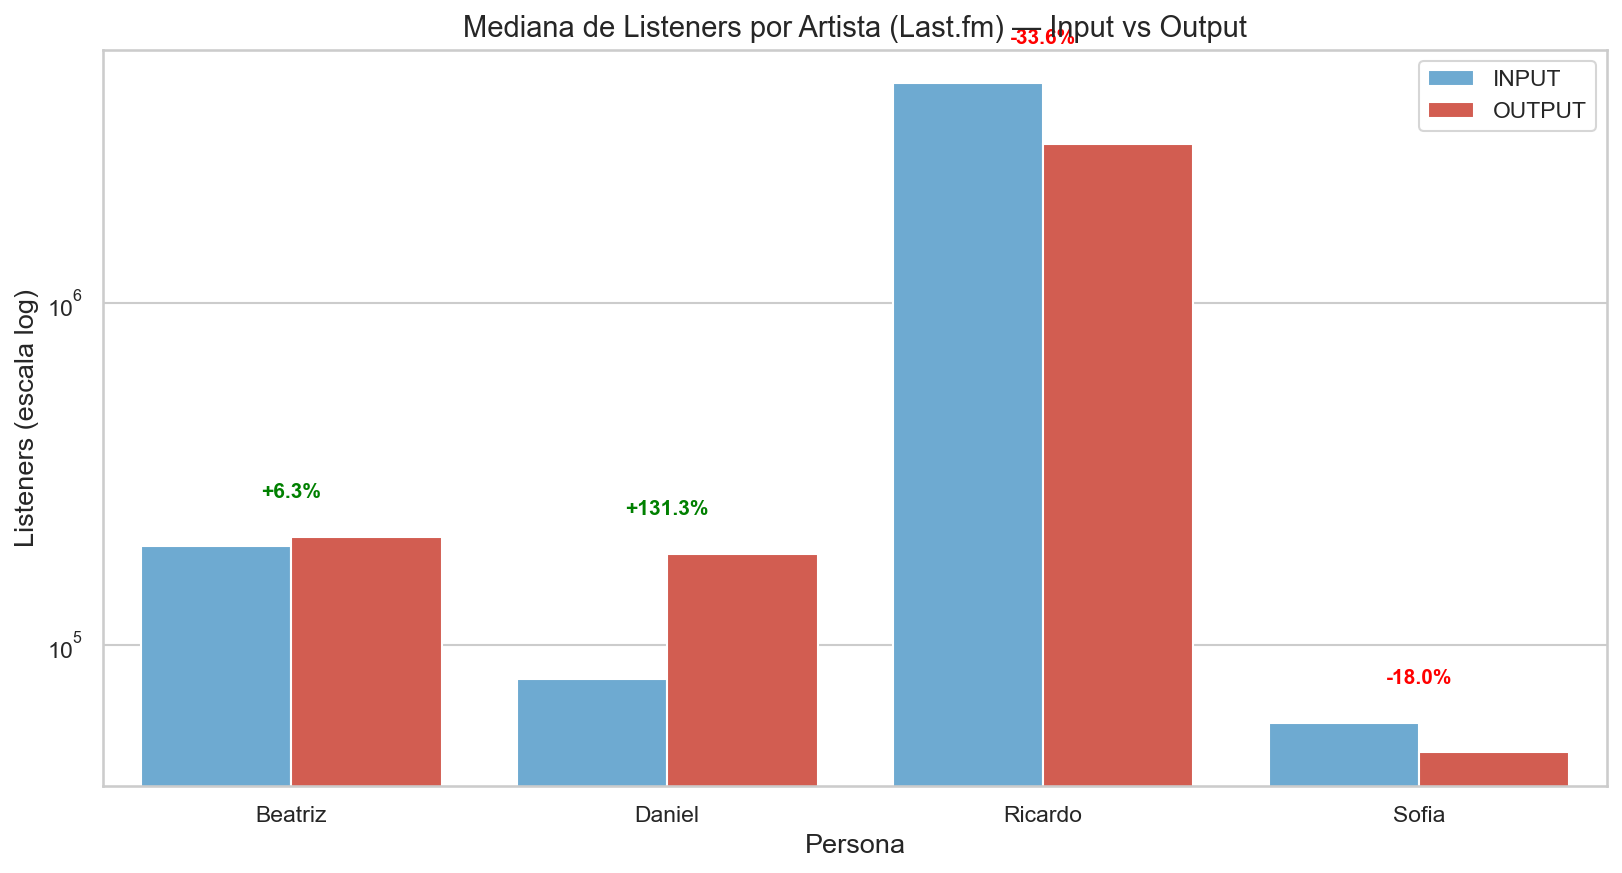
\includegraphics[width=0.85\textwidth]{cmp_bar_listeners.png}
\fontefig{Elaborado pelo autor (2026).}
\label{fig:bar-listeners}
\end{figure}

\noindent A coluna vermelha (\emph{Output}) de Daniel é visivelmente maior que a
azul (\emph{Input}); inversamente, Ricardo e Sofia têm a coluna \emph{Output}
menor. Adicionalmente, a Figura~\ref{fig:bar-solo} mostra a transformação na
estrutura social do consumo.

\begin{figure}[H]
\centering
\caption{Distribuição percentual de Solo (\emph{Person}) vs.\ Grupo (\emph{Group}) entre artistas únicos.}
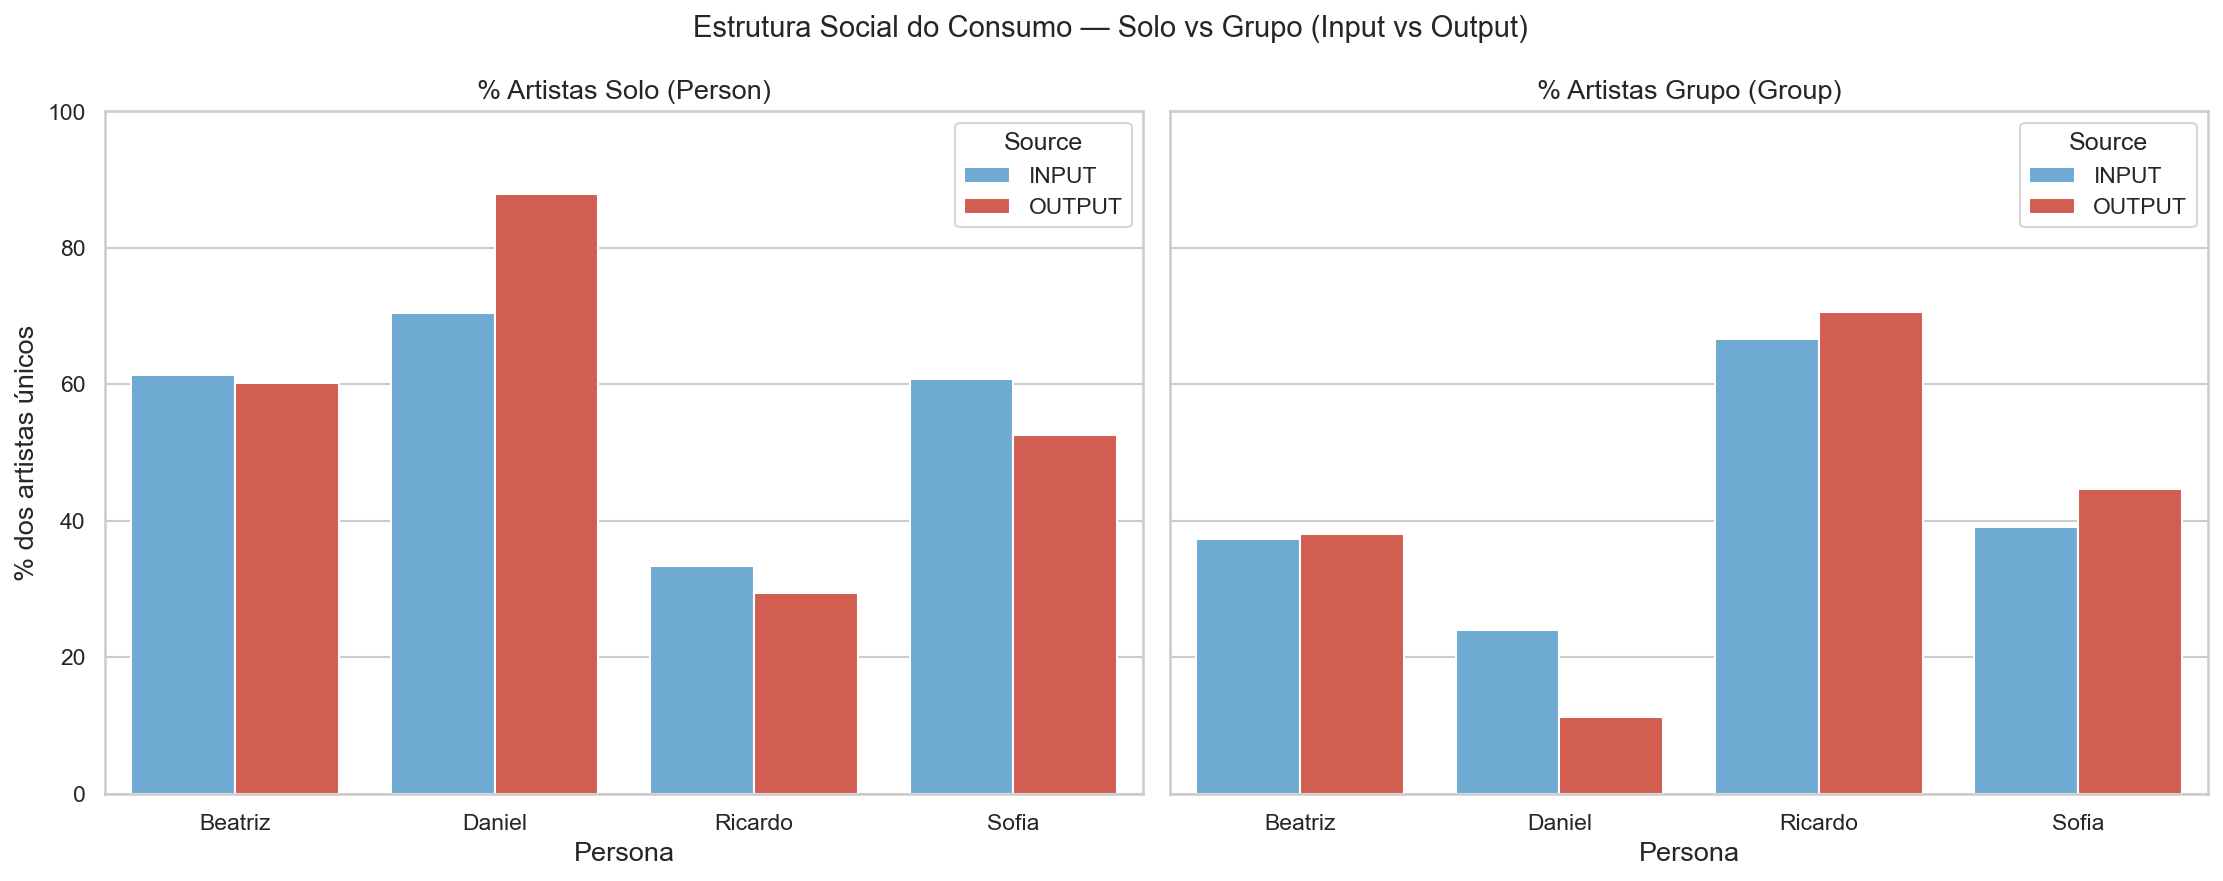
\includegraphics[width=0.85\textwidth]{cmp_bar_solo_group.png}
\fontefig{Elaborado pelo autor (2026).}
\label{fig:bar-solo}
\end{figure}

\noindent Daniel apresenta queda dramática de \% \emph{Group} (de $\sim$24\% para
$\sim$11\%, $\mathbf{-53{,}2\%}$), com correspondente aumento de \% Solo
($+24{,}7\%$). Esta queda de bandas/grupos confirma uma característica estrutural
do nicho \emph{lo-fi}: o ecossistema é dominado por \emph{bedroom producers}
individuais. O algoritmo, ao ``aprender'' o perfil de Daniel, acentua essa
característica social, recomendando ainda mais produtores solo do que o próprio
\emph{input} continha.

\textbf{Ressalva estatística.} A cobertura do campo de tipo de artista
(\texttt{mb\_artist\_type}) é satisfatória para Daniel (71,7\% no \emph{input},
93,0\% no \emph{output}); o cuidado necessário não é de cobertura, mas de
\textbf{base absoluta}: a categoria ``Grupo'' repousa sobre poucos artistas
($17 \rightarrow 12$ entre os tipados), e proporções sobre contagens pequenas têm
alta variância. O IC de Wilson 95\% do \% grupo (\emph{input} [15,5\%; 35,0\%]
vs.\ \emph{output} [6,5\%; 18,6\%]) apresenta sobreposição, de modo que o delta de
$-53\%$ deve ser lido como \emph{indício convergente}, e não como evidência
isolada. A direção do achado é, porém, corroborada de forma mais robusta pelo
aumento de \% solo ($+24{,}7\%$), que se apoia sobre base amostral maior
($50 \rightarrow 94$ artistas individuais únicos).

\textbf{Conclusão para Daniel.} Confirma-se a \textbf{hipótese de Contaminação
\emph{Pop}}. O algoritmo, ao buscar manter Daniel engajado, recomenda artistas
mais conhecidos dentro do nicho \emph{lo-fi}/instrumental, produtores que
migraram do anonimato para a ``elite do nicho'', evidenciando que a ``Zona de
Conforto Algorítmico'' desloca o perfil em direção ao centro de gravidade da
popularidade, mesmo dentro de um \emph{cluster} funcional/comoditizado. Este
resultado é coerente com a literatura sobre \emph{popularity bias} em recomendação
musical \cite{bauer2019global,kowald2020unfairness}.

\subsection{Sofia (Nicho): Viés do Hit dentro da Cauda Longa}

A persona Sofia, projetada como consumidora \emph{underground}/experimental,
apresenta o achado mais sutil e revelador do estudo. A análise das três principais
métricas relacionadas mostra um padrão paradoxal:

\begin{center}
\footnotesize
\begin{tabular}{l c c c}
\toprule
\textbf{Métrica} & \textbf{Input} & \textbf{Output} & \textbf{Delta} \\
\midrule
Listeners Mediano por \textbf{Artista} & 59.042 & 48.406 & $\mathbf{-18{,}0\%}$ \\
Listeners Mediano por \textbf{Track}   & 1.223  & 6.179  & $\mathbf{+405{,}2\%}$ \\
n.\ Artistas Únicos                    & 27     & 90     & $+233{,}3\%$ \\
\bottomrule
\end{tabular}
\end{center}

À primeira leitura, a queda de $-18\%$ nos \emph{listeners} por artista parece
sugerir que o algoritmo respeita o nicho de Sofia. Entretanto, a explosão de
$+405\%$ nos \emph{listeners} por \emph{track} revela um padrão diferente:
\textbf{o algoritmo respeita o nicho a nível de artista, mas dentro desses
artistas, prefere as faixas mais conhecidas}. Em outras palavras, ao invés de
recomendar \emph{deep cuts} obscuros (exatamente o comportamento de escuta
declarado de Sofia, com média de 7,41 faixas por artista), o sistema recomenda os
\emph{singles} mais expostos dos mesmos artistas \emph{indie}. A
Figura~\ref{fig:kde-era} mostra que a distribuição \emph{temporal} das faixas de
Sofia permanece estável entre \emph{input} e \emph{output}; o salto de
\emph{listeners} por faixa ($+405\%$; Tabela~\ref{tab:delta}), por sua vez, é
confirmado pelo teste de Mann-Whitney ($p \approx 1{,}3 \times 10^{-16}$),
revelando que, sob uma superfície temporal inalterada, a composição interna da
bolha mudou drasticamente.

\begin{figure}[H]
\centering
\caption{Distribuição temporal das faixas por persona (KDE, sobreposição \emph{Input}/\emph{Output}).}
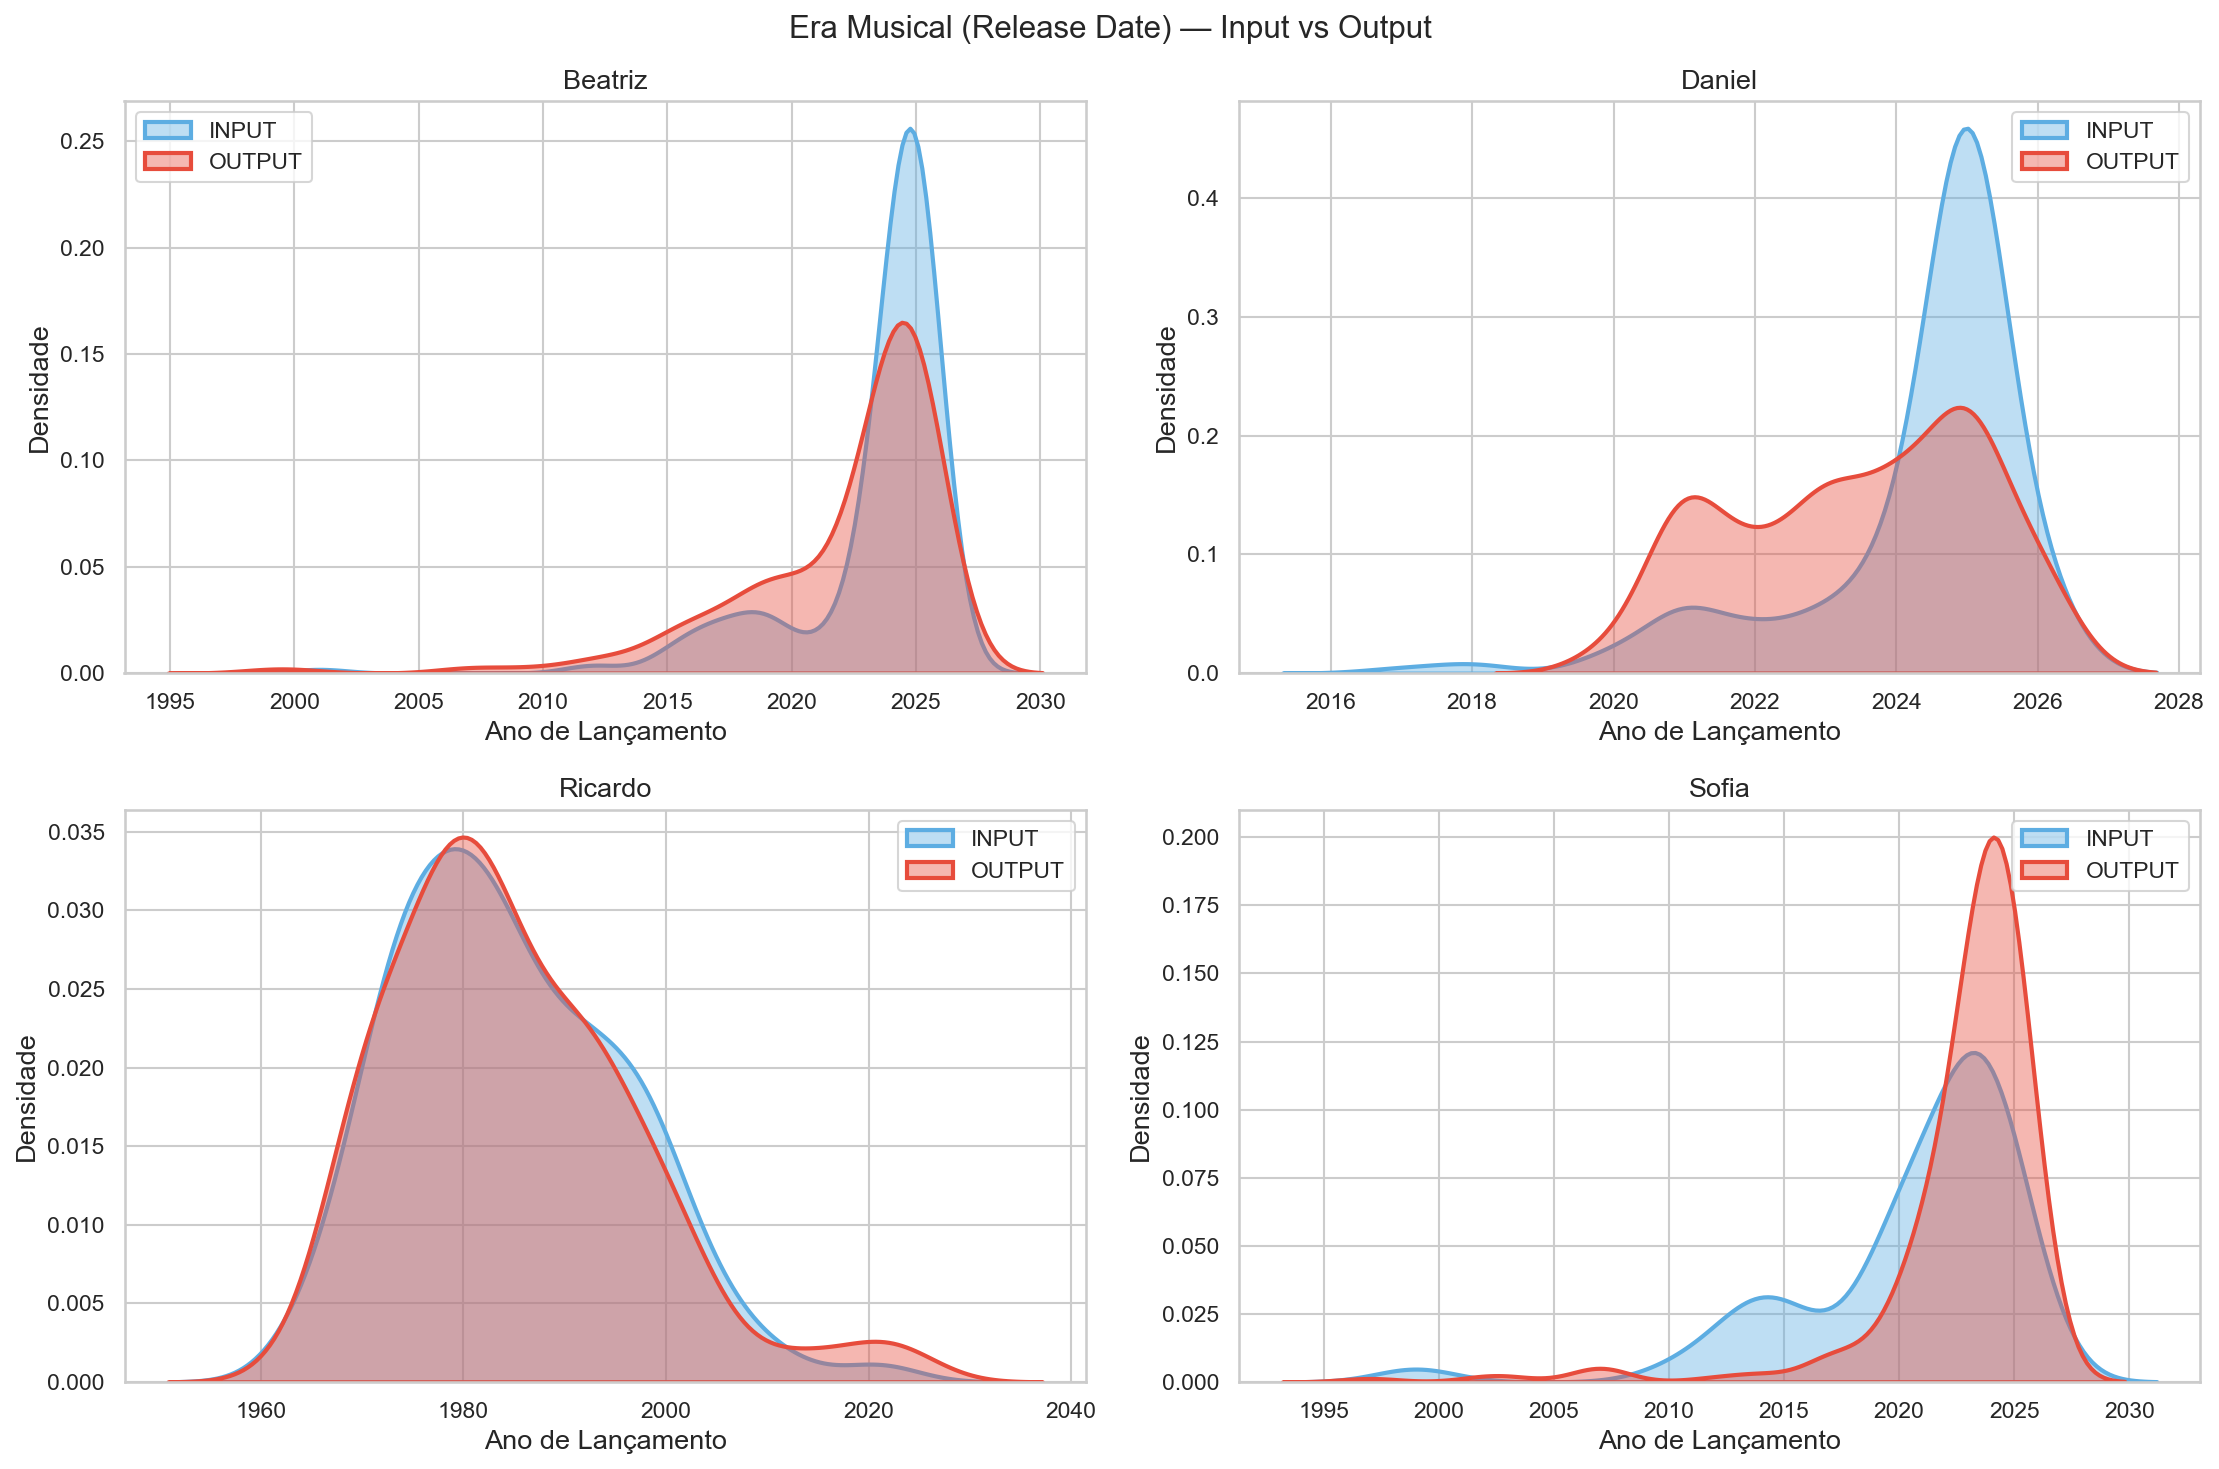
\includegraphics[width=0.95\textwidth]{cmp_kde_era.png}
\fontefig{Elaborado pelo autor (2026).}
\label{fig:kde-era}
\end{figure}

\noindent Adicionalmente, a expansão do leque de artistas ($+233{,}3\%$, de 27
para 90 artistas únicos) sugere que o algoritmo \textbf{fragmentou o consumo
profundo de Sofia}: em vez de deixá-la imersa em discografias completas
(S.Maharba, Eterna, Patch+, com 15+ faixas cada no \emph{input}), abriu o leque
para artistas adicionais com poucas faixas cada, comportamento típico de
``\emph{playlist} exploratória'' ao invés de ``escuta de álbum''.

\textbf{Conclusão para Sofia.} O algoritmo aplica um \textbf{viés de \emph{hit}
dentro da Cauda Longa}: respeita aparentemente o nicho (artistas igualmente
obscuros), mas força um padrão de escuta de ``\emph{singles}'' sobre o gosto
declarado por \emph{deep cuts} e discografia profunda. Adicionalmente, fragmenta
o consumo vertical
(poucos artistas, muitas faixas cada) em direção ao consumo horizontal (muitos
artistas, poucas faixas cada). Este achado refina a hipótese inicial: a
``gentrificação do nicho'' não acontece no eixo \emph{artista} (como
hipotetizado), mas no eixo \emph{faixa}, uma forma mais sutil de viés que
apenas a granularidade \emph{track-level} da fonte Last.fm permitiu capturar.

\subsection{Ricardo (Nostálgico): Pulverização da Fidelidade Canônica}

A persona Ricardo, projetada como consumidor saudosista (\emph{Album-Oriented
Rock} $+$ MPB clássica, 18 artistas com 11,11 faixas/artista em média), exibe os
\textbf{maiores deltas de todo o estudo} em três das métricas de diversidade:
n.\ Artistas Únicos $18 \rightarrow 126$ ($\mathbf{+600{,}0\%}$, o maior delta
absoluto em qualquer métrica/persona); Shannon \emph{Entropy}
$4{,}10 \rightarrow 6{,}61$ ($\mathbf{+61{,}4\%}$, a maior variação relativa de
entropia); e Coeficiente de Gini $0{,}18 \rightarrow 0{,}37$
($\mathbf{+110{,}8\%}$, duplicação da desigualdade).

Estes números indicam uma \textbf{pulverização sistemática da fidelidade
canônica} declarada por Ricardo. Ao invés de respeitar o comportamento de
``escuta de discografia profunda'' (mergulho vertical em poucos ídolos
consagrados), o algoritmo expandiu o leque de artistas em sete vezes, 
recomendando muitos artistas novos com poucas faixas cada, em vez de mais faixas
dos mesmos 18 artistas que Ricardo já declarou consumir. A
Figura~\ref{fig:tags} ilustra a transformação no \emph{Top} 10 de \emph{tags}.

\begin{figure}[H]
\centering
\caption{\emph{Top} 10 \emph{Tags} por Persona, lado a lado: \emph{Input} (azul) vs.\ \emph{Output} (vermelho).}
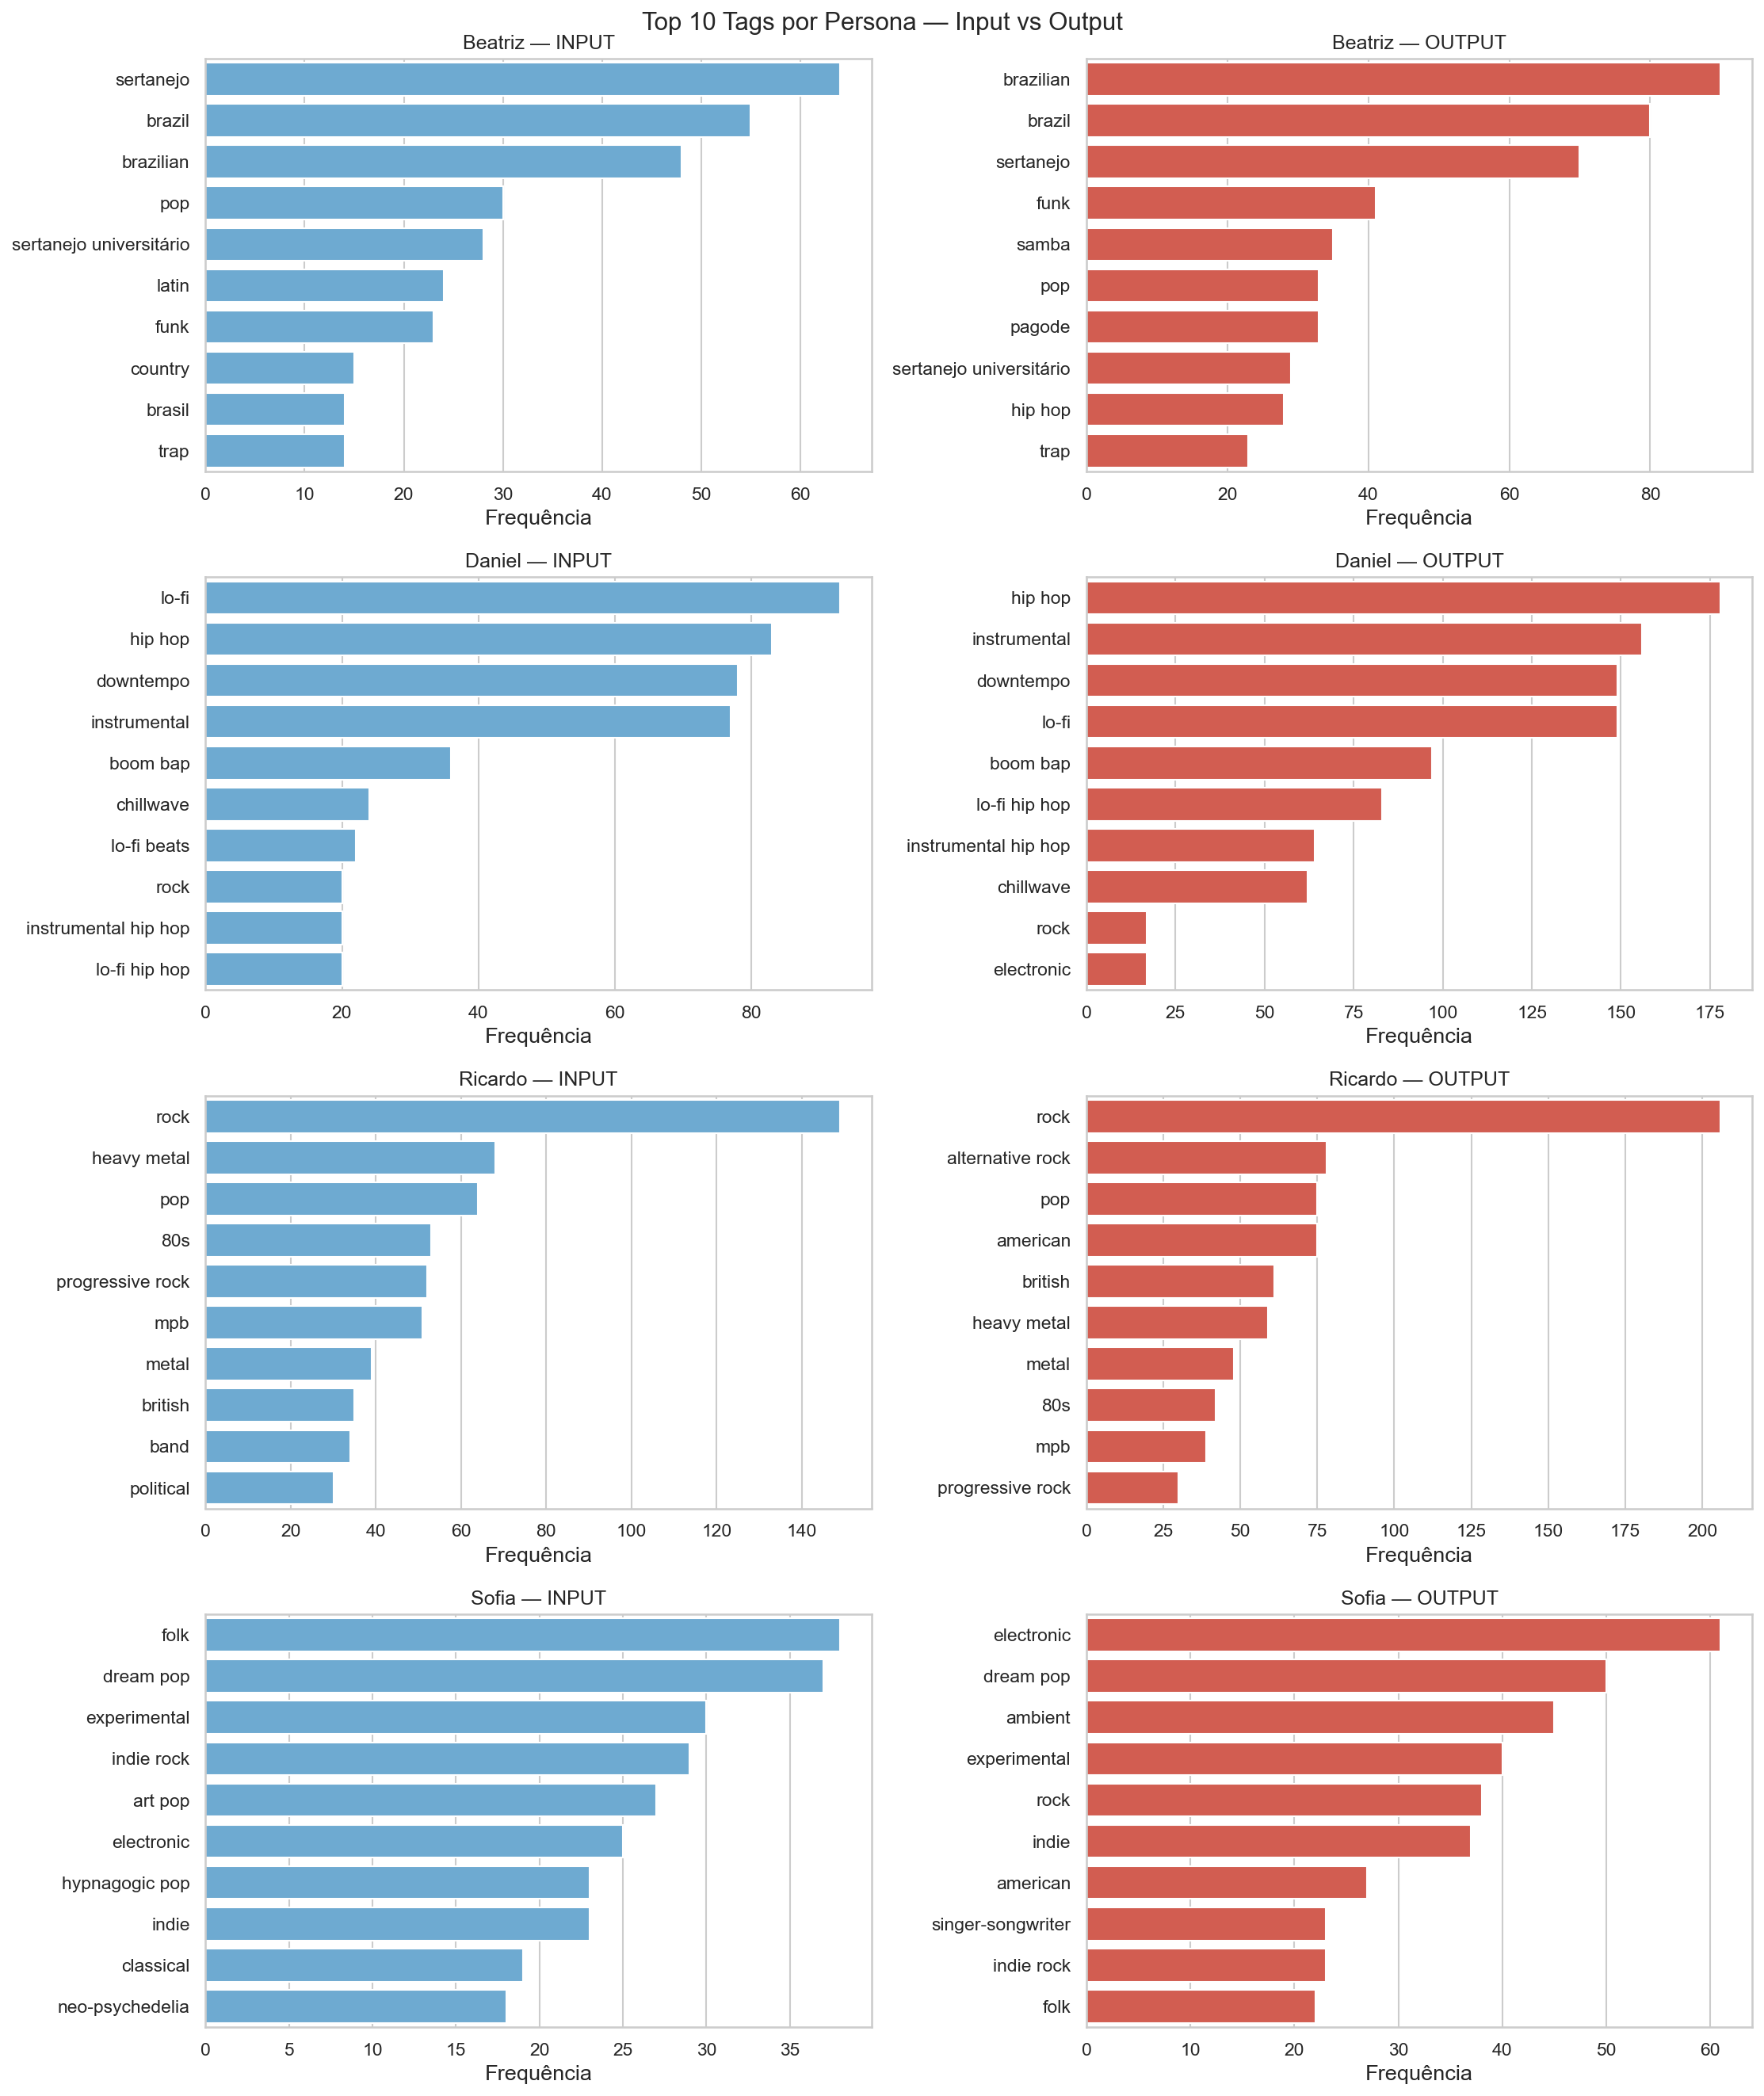
\includegraphics[width=0.95\textwidth]{cmp_tags.png}
\fontefig{Elaborado pelo autor (2026).}
\label{fig:tags}
\end{figure}

\noindent Ricardo mantém o domínio de \texttt{rock}, \texttt{classic rock},
\texttt{hard rock}, mas o \emph{output} introduz \emph{tags} novas como
\texttt{british}, \texttt{progressive rock} e \texttt{90s}, ampliando o espectro
temático.

Surpreendentemente, os \emph{listeners} e \emph{playcount} medianos por artista
\textbf{caem} ($-33{,}6\%$ e $-59{,}4\%$, respectivamente). Isso decorre
matematicamente da expansão do leque: os 18 artistas originais de Ricardo
(Metallica, Beatles, Queen, etc.) têm milhões de \emph{listeners}; os 108 novos
artistas introduzidos pelo algoritmo são em média menos consagrados, abaixando
a mediana global, mesmo que cada um individualmente seja popular.

A análise da \textbf{Era de Carreira} revela um deslocamento sutil mas
significativo: a mediana sobe de \textbf{1965 para 1970,5 ($+5$ anos)}. O
algoritmo, mesmo respeitando a temporalidade geral do perfil (Ano Médio do
\emph{release} permanece em 1985), modernizou de cinco anos a janela formativa dos
artistas recomendados: ao invés de Beatles (carreira iniciada em 1960), introduz
Bon Jovi (1983); ao invés de Rolling Stones (1962), introduz Bryan Adams (1976).
O perfil ``saudosista'' continua, mas é discretamente puxado em direção ao final
dos anos 1970 e 80.

\textbf{Conclusão para Ricardo.} Confirma-se a hipótese de \textbf{violação ativa
do ``\emph{Legacy Control}''}. O algoritmo \textbf{NÃO respeita o comportamento de
fidelidade canônica}, ao contrário, força a substituição de ``discografia
profunda'' por ``exploração horizontal de artistas similares''. Este achado tem
implicações cruciais para o argumento sobre \emph{bolha de filtro}: contraria a
expectativa intuitiva de que perfis ultra-concentrados ficariam ``presos'' em
\emph{loops} temporais. Na prática, o algoritmo faz o oposto: \textbf{arromba a
bolha vertical, fragmenta o gosto consolidado e empurra o usuário em direção a uma
horizontalidade comum}. Vale registrar que esse resultado, embora refute a
hipótese \emph{local} de estagnamento, é plenamente coerente com a mesma
\textbf{gravidade de popularidade} observada nas demais personas: o extremo
superior de Ricardo (audiência na casa dos milhões) é puxado \emph{para baixo}
(\emph{listeners} $-33{,}6\%$; carreira mediana $+5$ anos, rumo a artistas menos
canônicos), assim como o extremo inferior de Daniel é puxado \emph{para cima}.
Ricardo não é, portanto, uma anomalia que contradiz o estudo, mas mais uma
confirmação da regressão à média de popularidade.

\section{Reconfiguração da Diversidade: Expansão de Riqueza com Manutenção de Silos}
\label{sec:diversidade-output}

A análise integrada das quatro personas revela o \textbf{achado central deste
estudo}, mais sutil e mais robusto do que a hipótese inicial de um ``colapso
de contexto'' entendido como fusão dos perfis. Quando se decompõe a noção de
``convergência'' em três níveis distintos (conteúdo, tema e magnitude de
diversidade), os dados \textbf{refutam a homogeneização de conteúdo} e revelam um
fenômeno estratificado: o algoritmo expande a riqueza interna de cada perfil e os
aproxima \emph{tematicamente}, mas mantém os repertórios de artistas rigidamente
separados.

\subsection*{Nível 1: Conteúdo (artistas): silos preservados, não colapso}

\noindent\textbf{Nota sobre os eixos.} Este nível mede a sobreposição de artistas
\textbf{entre personas distintas}, e não a substituição de artistas
\textbf{dentro} de uma mesma persona (fenômeno tratado como expansão de riqueza
no Nível 3). São perguntas ortogonais: ainda que cada perfil receba dezenas de
artistas novos no \emph{output}, o que se verifica aqui é se algum desses
artistas passa a ser \emph{compartilhado} com outra persona.

A métrica direta da convergência entre personas é o Índice de Jaccard
\emph{cross-persona} sobre os conjuntos de artistas. O resultado é inequívoco: o
Jaccard médio dos seis pares é \textbf{exatamente 0,000 tanto no \emph{input}
quanto no \emph{output}}, os quatro conjuntos de artistas recomendados são
integralmente disjuntos (união de 452 artistas, idêntica à soma dos tamanhos). Um
teste de permutação (rótulos de persona reembaralhados, mil reamostragens,
correção de \citeonline{phipson2010permutation}) demonstra que essa separação é
\textbf{significativamente maior do que a esperada ao acaso}: dado o tamanho dos
conjuntos, esperar-se-ia um Jaccard de 0,142 (IC 95\% [0,125; 0,161]) por mero
sorteio, contra 0,000 observado ($p < 0{,}001$). Em vez de fundir os perfis, o
algoritmo preserva, e estatisticamente acentua, silos de repertório
distintos. O contraste é notável: mesmo tendo triplicado ou até sextuplicado o
número de artistas de cada perfil (Nível 3), o algoritmo não introduziu
\textbf{um único} artista compartilhado entre duas personas, razão pela qual a
disjunção observada é ainda mais acentuada do que a esperada ao acaso.

\subsection*{Nível 2: Tema (gêneros/tags): convergência parcial}

No nível temático, o quadro se inverte parcialmente: o Jaccard médio de
\emph{tags} sobe de \textbf{0,128 (\emph{input}) para 0,154 (\emph{output})}, com
aumento em todos os seis pares. Ou seja, embora os artistas permaneçam disjuntos,
as recomendações aproximam tematicamente os perfis. Essa dissociação entre
proximidade temática e disjunção de artistas é coerente com
\citeonline{anderson2020algorithmic}, cujo estudo na própria Spotify mede
diversidade por proximidade sonora (\emph{embeddings}) e não por riqueza de
artistas.

\begin{table}[H]
\centering
\caption{Jaccard médio cross-persona (6 pares) vs.\ nulo de permutação.}
\label{tab:jaccard}
\footnotesize
\begin{tabularx}{\textwidth}{>{\raggedright\arraybackslash}p{2.6cm} >{\centering\arraybackslash}p{1.5cm} >{\centering\arraybackslash}p{1.5cm} >{\centering\arraybackslash}p{2.6cm} X}
\toprule
\textbf{Nível de comparação} & \textbf{Jaccard Input} & \textbf{Jaccard Output} & \textbf{Esperado ao acaso (Output)} & \textbf{Veredito} \\
\midrule
Artistas (conteúdo) & 0,000 & 0,000 & 0,142 [0,125; 0,161] & Disjunção total; mais segregado que o acaso ($p < 0{,}001$). \\
Gêneros/tags (tema) & 0,128 & 0,154 & 0,201 [0,182; 0,220] & Convergência temática parcial ($+20\%$), porém ainda abaixo do acaso. \\
\bottomrule
\end{tabularx}
\fontefig{Elaborado pelo autor (2026).}
\end{table}

\subsection*{Nível 3: Magnitude da diversidade: convergência por expansão de riqueza}

Há, de fato, convergência da Entropia de Shannon para um patamar comum
($\sim$6,5), antes dispersa entre 4,10 e 6,27, uma redução de $\sim$75\% na
amplitude entre personas. A Figura~\ref{fig:bar-shannon} e a
Tabela~\ref{tab:shannon} sintetizam o fenômeno.

\begin{figure}[H]
\centering
\caption{Shannon \emph{Entropy} de Artistas, \emph{Input} (azul) vs.\ \emph{Output} (vermelho), com delta \% anotado.}
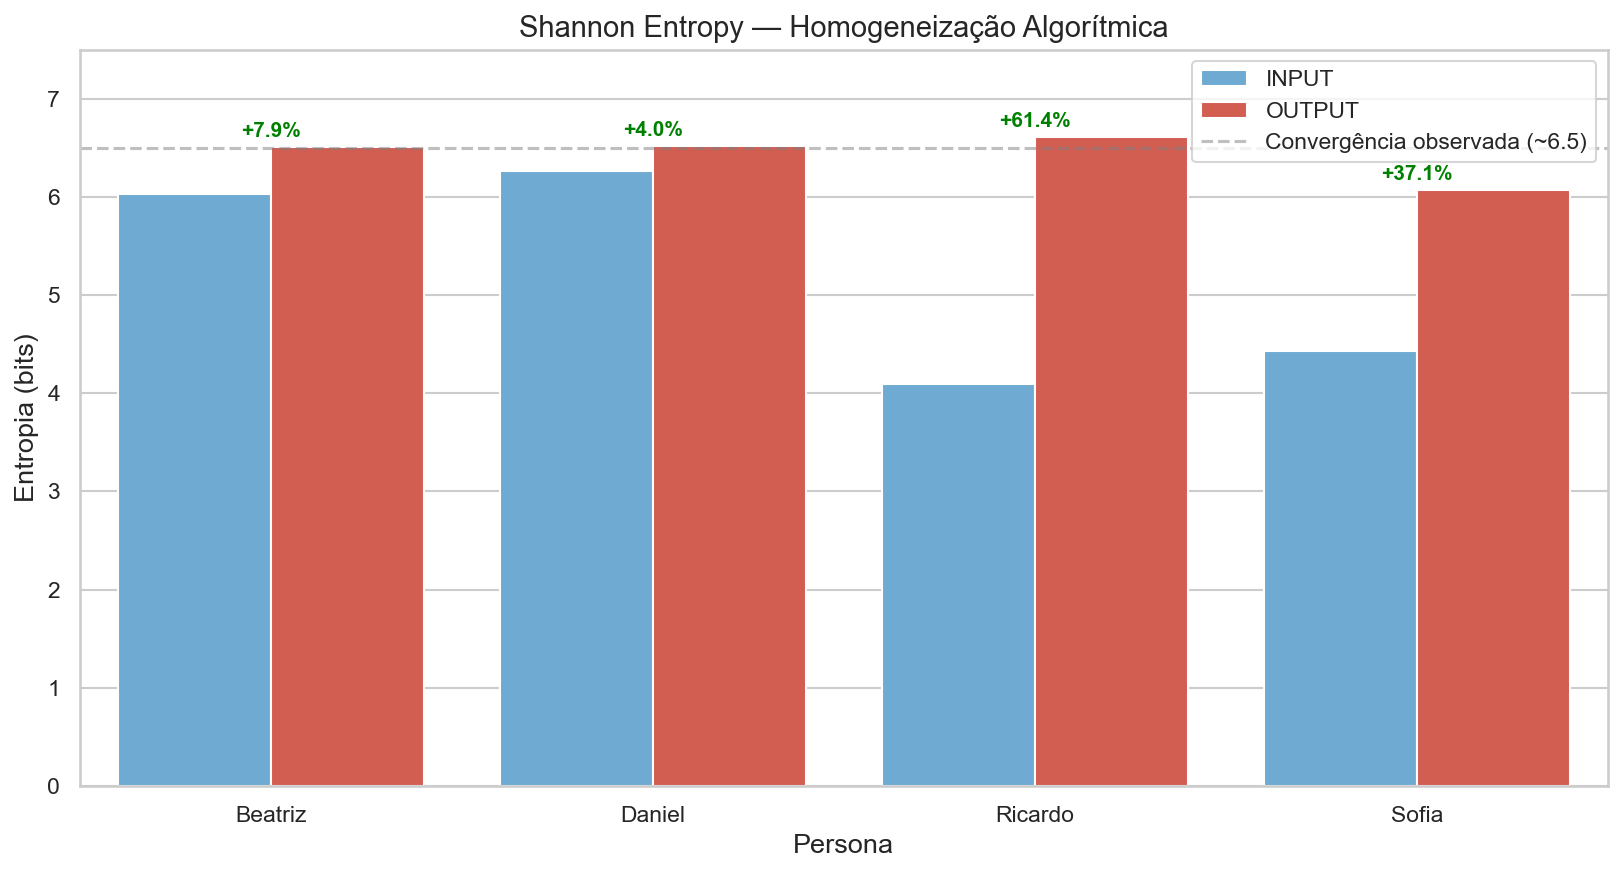
\includegraphics[width=0.85\textwidth]{cmp_bar_shannon.png}
\fontefig{Elaborado pelo autor (2026).}
\label{fig:bar-shannon}
\end{figure}

\noindent A linha tracejada cinza marca a faixa de convergência observada
($\sim$6,5).

\begin{table}[H]
\centering
\caption{Convergência da Shannon \emph{Entropy} (e a \emph{evenness} de Pielou).}
\label{tab:shannon}
\footnotesize
\begin{tabular}{>{\bfseries}l c c c c}
\toprule
\textbf{Persona} & \textbf{Shannon Input} & \textbf{Shannon Output} & \textbf{$\Delta$ relativo} & \textbf{Pielou In $\rightarrow$ Out} \\
\midrule
Beatriz & 6,03 & 6,51 & $+7{,}9\%$  & $0{,}92 \rightarrow 0{,}94$ \\
Daniel  & 6,27 & 6,52 & $+4{,}0\%$  & $0{,}95 \rightarrow 0{,}95$ \\
Ricardo & 4,10 & 6,61 & $\mathbf{+61{,}4\%}$ & $0{,}98 \rightarrow 0{,}95$ \\
Sofia   & 4,43 & 6,07 & $\mathbf{+37{,}1\%}$ & $0{,}93 \rightarrow 0{,}93$ \\
\bottomrule
\end{tabular}
\fontefig{Elaborado pelo autor (2026).}
\end{table}

Contudo, \textbf{essa convergência não é homogeneização de entropia, e sim
expansão de riqueza de catálogo}. A evidência é dupla. Primeiro, a \emph{evenness}
de Pielou permanece praticamente constante (0,92--0,98), para Ricardo, ela
inclusive \emph{cai} levemente ($0{,}98 \rightarrow 0{,}95$) enquanto a Shannon
dispara, prova de que o ganho vem do número de artistas ($18 \rightarrow 126$,
$+600\%$), não de maior uniformidade. Segundo, o controle por \textbf{rarefação}
(subamostragem do \emph{output} a $N = 200$ faixas, igual ao \emph{input};
\citeonline{gotelli2001quantifying}) confirma que o efeito não é artefato do maior
número de faixas: a riqueza de Ricardo mantém-se em \textbf{108 artistas (IC 95\%
[102; 113])} mesmo sob esforço amostral padronizado, contra 18 no \emph{input}. O
efeito persiste com robustez para Ricardo e Sofia; para Daniel, ao contrário, o
ganho de Shannon \textbf{perde significância após a rarefação} (IC 95\% [6,25;
6,44], que contém o valor de \emph{input}, 6,27), indicando que, nesse caso, parte
do ganho era mero artefato amostral.

\subsection*{Síntese: a bolha não se funde, alarga-se por dentro}

Os três níveis, considerados em conjunto, sustentam um achado mais forte que o
originalmente hipotetizado: \textbf{o algoritmo não homogeneíza o gosto entre
usuários}. Ele expande a riqueza interna de cada perfil (arrombando bolhas
verticais, como a de Ricardo) e os aproxima tematicamente, mas mantém repertórios
de artistas rigidamente disjuntos. O ``Colapso de Contexto'' anunciado nos
objetivos ocorre apenas no eixo temático e no de \emph{magnitude} de diversidade,
não no eixo de conteúdo. A bolha não se rompe nem se funde com as demais: ela
se alarga internamente enquanto suas paredes de conteúdo permanecem de pé.

\section{Síntese dos Achados e Discussão}

A Tabela~\ref{tab:sintese} consolida os achados centrais do estudo, mapeando-os
contra as hipóteses formuladas por persona no Capítulo~\ref{cap:metodologia}.

\begin{table}[H]
\centering
\caption{Síntese dos Achados por Persona e Hipóteses Confirmadas.}
\label{tab:sintese}
\footnotesize
\begin{tabularx}{\textwidth}{>{\bfseries\raggedright\arraybackslash}p{1.5cm} X X >{\centering\arraybackslash}p{1.8cm} >{\centering\arraybackslash}p{2.2cm}}
\toprule
\textbf{Persona} & \textbf{Hipótese Original} & \textbf{Achado Empírico} & \textbf{Magnitude} & \textbf{Status} \\
\midrule
Beatriz & \emph{Feedback loop} positivo blindando contra nicho & Mudanças tímidas, perfil \emph{mainstream} preservado & Baixa ($\sim$5--8\%) & Confirmada \\
Daniel & Contaminação \emph{Pop} dentro do nicho funcional & \emph{Listeners} $+131\%$, \emph{playcount} $+263\%$, \% Solo $+25\%$ & Alta ($\sim$131--263\%) & Confirmada \\
Sofia & Gentrificação do nicho de Cauda Longa & Viés do \emph{hit track-level} ($+405\%$), fragmentação vertical & Extrema (eixo \emph{track}) & Confirmada e refinada \\
Ricardo & Estagnamento de descoberta (\emph{loop} temporal) & Pulverização ($+600\%$); audiência puxada para baixo, coerente com a regressão à média & Extrema (diversidade) & Refutada localmente e reinterpretada \\
\bottomrule
\end{tabularx}
\fontefig{Elaborado pelo autor (2026).}
\end{table}

A hipótese de Ricardo merece destaque: o estudo havia antecipado que o algoritmo
poderia ``ficar preso'' em recomendações de eras passadas, gerando estagnamento de
descoberta. O resultado empírico aponta o oposto: o algoritmo arromba ativamente a
bolha vertical, introduzindo 108 novos artistas ($+600\%$) e modernizando
sutilmente a janela temporal ($+5$ anos na carreira mediana). Este achado é
cientificamente mais valioso do que a hipótese original, pois revela uma
\textbf{direcionalidade não-óbvia} do viés: o algoritmo prefere fragmentar
profundidade do que respeitá-la. Mais do que simplesmente refutar a hipótese, o
resultado a reposiciona: a fragmentação de Ricardo e o deslocamento de sua
audiência para baixo são a face, no extremo superior da distribuição, da mesma
gravidade que puxa Daniel para cima --- uma regressão à média de popularidade que
atravessa todas as personas.

\subsection{Os Quatro Achados Centrais}

Antes de enumerá-los, cabe explicitar a \textbf{moldura que os unifica}. Os
quatro achados a seguir não são fenômenos isolados: podem ser lidos como
manifestações de um único mecanismo, uma \textbf{``gravidade algorítmica'' que
desloca os perfis em direção a um patamar médio de popularidade} (regressão à
média). Daniel, na cauda, é puxado \emph{para cima}; Ricardo, no topo, é puxado
\emph{para baixo}; Sofia tem os artistas obscuros preservados, mas as faixas
empurradas para os \emph{hits}; e Beatriz, já próxima desse centro de gravidade,
quase não se move. Essa leitura, cujos mecanismos prováveis se discutem na
Seção 4.6.2, confere coerência ao conjunto dos resultados por
persona: o que parecia um catálogo de vieses heterogêneos é, no fundo, a mesma
força atuando sobre pontos diferentes da distribuição.

\textbf{1. Expansão de Riqueza com Manutenção de Silos.} O Spotify converge a
\emph{magnitude} de diversidade dos perfis para uma faixa estreita de Shannon
($\sim$6,5 \emph{bits}), mas, como provam a \emph{evenness} de Pielou plana e a
rarefação, isso é expansão de riqueza de catálogo, não homogeneização de
entropia. Crucialmente, no nível de conteúdo não há convergência alguma: o
Jaccard \emph{cross-persona} de artistas é 0,000, mais segregado que o acaso
($p < 0{,}001$). O algoritmo aproxima os perfis tematicamente (Jaccard de
\emph{tags} $+20\%$) enquanto mantém os repertórios de artistas disjuntos. Este é
o achado mais robusto e contraintuitivo do estudo.

\textbf{2. Viés de Popularidade Direcionalmente Dependente.} Daniel (perfil
moderado de nicho) é puxado \emph{para cima} em \emph{listeners} ($+131\%$);
Ricardo (perfil de \emph{superstars}) é puxado \emph{para baixo} ($-34\%$). Em
ambos os casos, a direção converge para um patamar médio de visibilidade,
evidenciando uma ``gravidade algorítmica'' que repele os extremos.

\textbf{3. Viés de \emph{Hit} dentro da Cauda Longa.} O algoritmo respeita a
Cauda Longa a nível de artista (Sofia mantém artistas obscuros), mas força
\emph{hits} a nível de faixa ($+405\%$ \emph{listeners} por \emph{track}). A
fragmentação do \emph{track-level} é uma forma de viés mais sutil que o eixo
\emph{artist-level} não captura.

\textbf{4. Pulverização da Fidelidade Canônica.} Perfis verticais (escuta de
álbum) são sistematicamente fragmentados em horizontais (escuta de
\emph{playlist}). O algoritmo prefere expansão de catálogo a profundidade
discográfica, mesmo quando o sinal de gosto declarado aponta no sentido oposto.

\subsection{Implicações Teóricas e Sociotécnicas}

Os quatro achados, considerados em conjunto, sustentam o argumento central da
pesquisa: o algoritmo do Spotify, longe de ser um espelho neutro do gosto
declarado, opera como \textbf{um prisma com geometria conhecida}. Sua geometria
privilegia (i) horizontalidade sobre verticalidade, (ii) artistas medianos sobre
extremos (\emph{superstars} ou \emph{underground} absolutos), e (iii) faixas
reconhecíveis sobre \emph{deep cuts}, em coerência com o modelo de negócio da
Economia da Atenção.

\textbf{Mecanismos plausíveis (inferidos).} Sendo esta uma auditoria de
caixa-preta, os mecanismos internos do recomendador são inobserváveis por
construção; ainda assim, os padrões medidos são compatíveis com hipóteses de
mecanismo bem estabelecidas na literatura técnica referida na Introdução
(Filtragem Colaborativa, Processamento de Linguagem Natural e \emph{Deep
Learning}). A \textbf{gravidade em direção à média de popularidade} (Daniel
$\uparrow$, Ricardo $\downarrow$) é o comportamento esperado de uma
\textbf{filtragem colaborativa}: itens co-consumidos por muitos vizinhos
tornam-se coocorrências frequentes, de modo que perfis situados nos extremos da
distribuição são atraídos para regiões de maior densidade de dados de
engajamento. O \textbf{viés de \emph{hit} no nível da faixa} (Sofia) é compatível
com um sinal de treino \textbf{ponderado por volume de reprodução}: dentro de um
mesmo artista, a faixa mais tocada domina a vizinhança de recomendação,
deslocando \emph{deep cuts} para \emph{singles}. Por fim, a \textbf{pulverização
de perfis ultra-concentrados} (Ricardo) é coerente com a \textbf{suavização no
espaço de \emph{embeddings}}: poucos artistas densamente repetidos deixam ampla
margem para o preenchimento com vizinhos sonoros, fragmentando a profundidade
discográfica em horizontalidade. Reforça-se que se trata de \emph{hipóteses de
mecanismo}, e não de observações diretas do sistema, cuja verificação exigiria
acesso interno hoje vedado pela opacidade documentada nesta pesquisa.

A Onda 3 da restrição da API, que removeu silenciosamente os campos
\texttt{popularity}, \texttt{followers} e \texttt{genres} durante a execução desta
pesquisa, corrobora institucionalmente o argumento: a plataforma opera para
preservar opacidade sobre exatamente as variáveis que permitem auditá-la
externamente. Esta meta-evidência confere robustez epistemológica adicional aos
achados quantitativos.

A Cauda Longa, central na literatura de economia digital
\cite{anderson2006longtail}, revela-se acessível apenas parcialmente: o algoritmo
permite ao usuário \emph{visitar} artistas de nicho, mas o conduz pelos
\emph{singles} consagrados desses artistas, uma forma de ``Cauda Longa
Curada''. Para o pesquisador interessado em diversidade cultural, não basta
perguntar \emph{se} o algoritmo recomenda nicho; é preciso perguntar \emph{como}
ele recomenda nicho, preocupação que dialoga com a literatura de \emph{fairness}
para fornecedores e a defesa de \emph{marketplaces} equilibrados
\cite{mehrotra2018towards}.

\textbf{Diálogo com a literatura.} \citeonline{anderson2020algorithmic} reportam
que a personalização tende a \emph{reduzir} a diversidade de consumo medida por
\emph{embeddings} (proximidade sonora), aparente contradição com a elevação de
diversidade aqui observada. Os resultados são, porém, compatíveis quando se
distingue a \emph{riqueza de artistas} (que sobe, por expansão de catálogo) da
\emph{proximidade no espaço sonoro} (que pode convergir). O resultado também
ressoa com \citeonline{hosanagar2014will}, que observam que sistemas de
recomendação podem \emph{aumentar} a comunalidade entre usuários, aqui, essa
comunalidade aparece no nível temático (Jaccard de \emph{tags} $\uparrow$), mas
não no de conteúdo (Jaccard de artistas $= 0$). Por fim, trabalhos recentes de
auditoria e \emph{fairness} em \emph{streaming} musical
\cite{turnbull2022exploring,matrosova2024recommender,shakespeare2025reframing}
confirmam a atualidade do problema.

\subsection{Limitações Específicas dos Resultados deste Capítulo}

Além das limitações gerais já discutidas na Seção~\ref{sec:limitacoes}, dois
pontos específicos merecem registro:

\begin{itemize}
  \item \textbf{Janela temporal única de coleta:} os \emph{outputs} analisados
  refletem o estado dos \emph{Daily Mixes} na semana de 28/04/2026; o algoritmo é
  dinâmico e estes valores podem variar em coletas longitudinais.
  \item \textbf{Cobertura desigual de \texttt{mb\_career\_start}:} a métrica de
  Era de Carreira tem cobertura integral (100\%) para Ricardo, mas baixa (20\%)
  para Daniel (produtores \emph{lo-fi} obscuros frequentemente ausentes do
  catálogo institucional).
\end{itemize}

Apesar dessas limitações, a triangulação metodológica adotada (Shannon, Gini,
HHI, \emph{Listeners}, \emph{Playcount}, Era de Carreira, Tipo de Artista, sete
famílias de métricas independentes) e o uso de duas fontes externas consagradas
na literatura de recuperação de informação musical
(Last.fm $+$ MusicBrainz) conferem ao conjunto de achados uma robustez que
justifica os resultados aqui apresentados como \textbf{evidência empírica forte e
auditável} da governança algorítmica do Spotify sobre a diversidade musical de
seus usuários.

% ==========================================================
\chapter{Considerações Finais}
% ==========================================================

Este trabalho teve como objetivo geral auditar o comportamento do sistema de
recomendação do Spotify, por meio de uma metodologia de caixa-preta com personas
sintéticas, a fim de mensurar o impacto da curadoria algorítmica sobre a
diversidade cultural. O conjunto de evidências reunido permite responder
afirmativamente à pergunta condutora, o algoritmo interfere de modo sistemático
e mensurável sobre o gosto declarado, mas exige refinar a forma como essa
interferência é compreendida.

Quanto aos objetivos específicos, todos foram cumpridos. Primeiro, os quatro
arquétipos de consumo foram modelados e implementados em contas reais,
traduzindo perfis psicográficos em \emph{datasets} controlados. Segundo, a
heterogeneidade e o isolamento dos \emph{inputs} foram validados
estatisticamente: o Índice de Jaccard nulo entre as personas confirmou a
ortogonalidade da linha de base (\emph{cold start}). Terceiro, os metadados das
recomendações (\emph{Daily Mixes}) foram coletados e processados, contornando-se a
obstrução progressiva da \emph{Web API} por meio de \emph{playlists} espelho e do
enriquecimento via Last.fm e MusicBrainz. Quarto, a diversidade e a concentração
foram mensuradas por um conjunto triangulado de indicadores, Entropia de
Shannon, \emph{evenness} de Pielou, Coeficiente de Gini, HHI e Jaccard,
acompanhados de tratamento estatístico inferencial.

O achado central revelou-se mais sutil do que a hipótese inicial de um ``colapso
de contexto'' entendido como fusão dos perfis. Decomposta a noção de convergência
em três níveis, observou-se que: no nível do \textbf{conteúdo}, os repertórios de
artistas das quatro personas permanecem integralmente disjuntos (Jaccard $= 0$),
de forma estatisticamente mais segregada do que o acaso ($p < 0{,}001$); no nível
\textbf{temático}, há convergência parcial de gêneros (Jaccard de \emph{tags} de
0,128 para 0,154); e no nível da \textbf{magnitude da diversidade}, a aparente
convergência da Entropia de Shannon é, na realidade, expansão de riqueza de
catálogo, comprovada pela \emph{evenness} de Pielou praticamente constante e
pela análise de rarefação, e não homogeneização de entropia. Assim, o
algoritmo não homogeneíza o gosto entre usuários: ele alarga internamente a bolha
de cada perfil e os aproxima tematicamente, mas preserva paredes de conteúdo
distintas.

A esse achado somam-se vieses direcionais bem definidos: uma ``gravidade
algorítmica'' que desloca perfis em direção a um patamar médio de popularidade
(Daniel, $+131\%$ de ouvintes por artista) e um viés de \emph{hit} que, mesmo
respeitando a cauda longa no eixo do artista, força as faixas mais expostas no
eixo da obra (Sofia, $+405\%$ de ouvintes por faixa). De modo contraintuitivo, o
perfil de fidelidade canônica (Ricardo) teve sua bolha vertical arrombada, com
expansão de 18 para 126 artistas, o oposto do estagnamento temporal
hipotetizado.

Como contribuições, o trabalho (i) oferece evidência empírica, inferencialmente
sustentada, da geometria de viés do recomendador do Spotify para o mercado
brasileiro; (ii) demonstra a importância metodológica de separar \emph{riqueza}
de \emph{uniformidade} e \emph{conteúdo} de \emph{tema} na medição de
diversidade, evitando conclusões equivocadas a partir da Entropia de Shannon
bruta; e (iii) documenta, como meta-evidência, a obstrução progressiva e
unilateral da \emph{Web API} durante a própria execução da auditoria, 
ilustração concreta da opacidade e da assimetria informacional que motivam, sob a
ótica da Gestão da Informação, a agenda de auditoria algorítmica.

Duas dessas contribuições merecem destaque por seu alcance para além do caso do
Spotify. A primeira é de ordem \textbf{conceitual e transferível}: a decomposição
da noção de ``convergência'' em três eixos independentes --- \textbf{conteúdo}
(sobreposição de artistas), \textbf{tema} (gêneros/\emph{tags}) e
\textbf{magnitude} de diversidade (entropia, por sua vez decomposta em riqueza e
uniformidade) --- constitui um instrumento analítico reaproveitável por outras
auditorias de recomendadores, que com frequência tratam a ``homogeneização''
como um bloco único e indiferenciado. A segunda é de ordem \textbf{teórica}: o
\textbf{viés de \emph{hit} dentro da cauda longa} --- a distinção entre respeitar
o nicho no eixo do \emph{artista}, mas não no eixo da \emph{faixa} --- refina a
literatura de \emph{popularity bias}, que raramente separa esses dois níveis de
granularidade.

No plano \textbf{normativo e prático}, sob a ótica da Gestão da Informação, os
achados sustentam uma agenda concreta. Para o \textbf{ouvinte}, evidenciam que
``acessar o nicho'' não equivale a ``escapar do \emph{hit}'', o que reposiciona o
debate sobre autonomia informacional e serendipidade: a diversidade oferecida é
real em riqueza, mas curada em direção ao reconhecível. Para o \textbf{artista de
cauda longa} (o fornecedor do \emph{marketplace}), mostram que a visibilidade
algorítmica tende a se concentrar nos \emph{singles} já consagrados, com
implicações diretas de \emph{fairness} de fornecedor. E para o \textbf{gestor da
informação e o regulador}, reforçam a urgência de mecanismos de transparência,
auditabilidade e portabilidade de dados que reduzam a assimetria informacional
entre plataforma e sociedade --- a mesma assimetria que a obstrução progressiva
da API, testemunhada ao vivo durante esta pesquisa, tornou palpável.

Reconhecem-se as limitações do estudo: a coleta constitui um \emph{snapshot}
temporal único, conduzido com quatro agentes e em um único mercado (Brasil); as
fontes externas, sobretudo o Last.fm, apresentam viés de cobertura geocultural
que torna as comparações \emph{cross-persona} de magnitude absoluta menos
robustas que os deltas \emph{within-persona}; e a métrica de diversidade temática
depende de \emph{tags} de granularidade heterogênea.

Como agenda futura, recomendam-se estudos longitudinais que acompanhem a evolução
das recomendações ao longo do tempo; a ampliação do número de personas e a
replicação em outros mercados culturais; a incorporação de métricas de
diversidade baseadas em \emph{embeddings} sonoros, que permitiriam o diálogo
direto com a literatura da própria indústria; e a investigação de mecanismos de
transparência e auditabilidade que reduzam a assimetria informacional aqui
evidenciada. Em síntese, mais do que perguntar \emph{se} o algoritmo recomenda
nicho, esta pesquisa demonstra a importância de perguntar \emph{como} ele o faz,
distinção decisiva para o debate sobre diversidade cultural na era da
governança algorítmica.

% ----------------------------------------------------------
% ELEMENTOS PÓS-TEXTUAIS
% ----------------------------------------------------------
\postextual

% ----------------------------------------------------------
% Referências bibliográficas
% ----------------------------------------------------------
\bibliography{referencias}

% ==========================================================
% APENDICE A -- Listas de Artistas por Persona (gerado automaticamente)
% ==========================================================
\begin{apendicesenv}
\chapter{Listas de Artistas por Persona (\emph{Input} e \emph{Output})}

\noindent Relação dos artistas únicos (identificados por \texttt{primary\_artist\_name}) que compõem os estímulos declarados (\emph{input}) e as recomendações algorítmicas coletadas (\emph{output}) de cada persona. Elaboração própria do autor (2026), a partir dos dados coletados via Spotify e enriquecidos com Last.fm e MusicBrainz. Estas listas sustentam empiricamente o Índice de Jaccard cross-persona igual a zero discutido na Seção~\ref{sec:diversidade-output}: não há um único artista compartilhado entre personas distintas.

\section*{A.1\quad Beatriz (Mainstream)}
\addcontentsline{toc}{section}{A.1 Beatriz (Mainstream)}

\noindent\textbf{Input (estímulo declarado) --- 94 artistas:} AgroPlay; Ana Castela; Anitta; BLOW RECORDS; Brenno \& Matheus; Bruno \& Barretto; Bruno Rosa; Burna Boy; cjnobeat; Clayton \& Romário; CountryBeat; Danilo e Davi; Dave; Diego \& Arnaldo; Diego \& Victor Hugo; DJ BRIZY; Dj Caio Vieira; Dj GBR; Dj GM; Dj Guuh; DJ Japa NK; Dj Luan Gomes; DJ NATAN 22; DJ Oreia; DJ Ryder; Dj Yuri Pedrada; Eric Land; Felipe Amorim; Felipe e Rodrigo; Ferrugem; FloyyMenor; Grupo Chocolate; Grupo Menos É Mais; Guilherme \& Benuto; Gunna; Gusttavo Lima; Henrique \& Juliano; Hugo \& Guilherme; J. Eskine; Jennifer e Stephany; Jmilton; Jorge \& Mateus; KayBlack; Lauana Prado; Lu \& Rayane; Luan Pereira; Luis Fonsi; Léo Santana; Mari Fernandez; Matheus \& Kauan; Matheus Fernandes; Matheus Vargas; Matuê; Mayke \& Rodrigo; MC Cebezinho; MC GP; Mc IG; MC Jvila; Mc Lele JP; MC LUUKY; MC Marks; MC Meno K; Mc Negão Original; Mc Rodrigo do CN; MC Ryan SP; MC Tuto; MC Willian; Murilo Huff; Nagalli; Naiara Azevedo; Natanzinho Lima; NATTAN; Orochi; Oruam; Panda; Pedro Paulo \& Alex; PEDRO SAMPAIO; Rafa e Junior; Repsaj; Ricky Martin; Simone Mendes; Som de Faculdade; Sorriso Maroto; Suel; Thales Lessa; The Weeknd; Turma do Pagode; US Agroboy; Veigh; Vitinho Imperador; Wesley Safadão; WIU; Yasmin Sensação; Zé Neto \& Cristiano.


\noindent\textbf{Output (recomendações) --- 121 artistas:} AgroPlay; Ana Castela; Anitta; Atitude 67; Belo; BK; Bruno \& Barretto; Bruno \& Marrone; Clayton \& Romário; Cristiano Araújo; Delacruz; Di Propósito; Diego \& Victor Hugo; Dilsinho; Diogo Nogueira; DJ BRIZY; Dj GBR; Dj Guuh; DJ Japa NK; DJ NATAN 22; DJ Oreia; Dj Yuri Pedrada; DJ Zigão; Eric Land; Exaltasamba; Felipe Amorim; Felipe Araújo; Felipe e Rodrigo; Fernando \& Sorocaba; Ferrugem; Filho do Piseiro; George Henrique \& Rodrigo; Grupo Chocolate; Grupo Menos É Mais; Grupo Revelação; Guilherme \& Benuto; Guilherme \& Santiago; Gustavo Mioto; Gusttavo Lima; Henrique \& Juliano; Henrique Casttro; Henry Freitas; Hugo \& Guilherme; Humberto \& Ronaldo; Hungria; Israel \& Rodolffo; Jads \& Jadson; Jorge \& Mateus; Jorge Aragão; João Gomes; Juan Marcus \& Vinícius; Kamisa 10; KayBlack; Lauana Prado; Luan Pereira; Luan Santana; LUDMILLA; Léo Foguete; Léo Santana; Mari Fernandez; Marvvila; Marília Mendonça; Matheus \& Kauan; Matheus Fernandes; Matheus Vargas; Matuê; Mayke \& Rodrigo; MC Cebezinho; Mc Daniel; Mc Davi; Mc Don Juan; MC Du Black; MC GP; Mc IG; Mc Jacaré; Mc Kevin; Mc Lele JP; Mc Leozin; MC Marks; MC Meno K; MC Menor da VG; MC Neguinho do Kaxeta; Mc Negão Original; Mc Paiva ZS; MC PH; Mc Rodrigo do CN; MC Ryan SP; MC Tuto; Mumuzinho; Murilo Huff; Natanzinho Lima; NATTAN; Orochi; Os Barões Da Pisadinha; Pablo; Panda; PEDRO SAMPAIO; Perera DJ; Pixote; Péricles; Rey Vaqueiro; Simone Mendes; Sorriso Maroto; Sotam; Soweto; Suel; Talita Mel; THE BOX; Thiaguinho; Turma do Pagode; Tz da Coronel; Veigh; Vitinho; Vitinho Imperador; Vou Zuar; Vulgo FK; Wesley Safadão; WIU; Yan; Zé Neto \& Cristiano; Zé Vaqueiro.

\section*{A.2\quad Daniel (Lo-fi/Funcional)}
\addcontentsline{toc}{section}{A.2 Daniel (Lo-fi/Funcional)}

\noindent\textbf{Input (estímulo declarado) --- 99 artistas:} \$imba; Ali Kaj; Alto; Ambulo; amies; Analogue Alf; Banks; Bcalm; Beats on 21st; BeatsBySindri; Breezonic; Bring Me The Horizon; butterfli; Cloudroom; Corridor; Cozeen; cxlt.; deadman; Dimension 32; Dosi; Dozy Duzzn; DreamWavez; Dry Season; Erwin Do; Flitz\&Suppe; Floating Basket; fnonose; Fracta Aurea; Frances The Mute; French Connection; Fya Playce; Golden Mist; Goson; heirloom; Hevi; HM Surf; Hoogway; Indigo Songs; jaackson; Jazzamass; jean opal; Juliàn; jxsn; Kainbeats; KiddoCalvin; Leavv; Lenny Loops; lil francky; Lil Leaf; lilibu; Lofi Girl; loutwo; low pines; marsquake; mell-ø; mellow fox; Mellow Melt; Mellow Mirror; mommy; Mondo Loops; morningtime; Mujo; Muroki; mxgnetic.; nate2timez; new vibe; No Spirit; Notation; Oh, My.; Oroshi; Osian Lewis; ourchase; pete castle; Philanthrope; Phlocalyst; Photosynthetic; Plaxon; Project AER; sad notes; saint rumi; sellar; Sleepr Cell; slowburn; Slowday; Smith Beats; softflow; softy; Soulflu; Space Queen; Spring Bingo; Sunny Léo; Sátyr; Theo Aabel; Tooslo; Towerz; xander.; Yasumu; Youthology; Yumeoka.


\noindent\textbf{Output (recomendações) --- 115 artistas:} after noon; Alto; amies; Bcalm; Bert; Blue Fox; Blue Wednesday; BluntOne; Breezonic; BVG; Charlee Nguyen; Chiccote's Beats; Cloudroom; cxlt.; Dosi; dryhope; eleven; ENRA; entsy; eugenio izzi; Floating Basket; fnonose; fosse; fourwalls; gCoope; Gerardo Millán; Golden Mist; Goofy Cat; Goson; H.1; Haku-San; Hevi; HM Surf; Hoogway; idylla; Indigo Songs; Intoku; j'san; Jhove; Juliàn; Julián Aponte; juniorodeo; jxsn; Kainbeats; Kanisan; Khutko; KioKo; Krynoze; kudo; Kupla; Kurt Stewart; Ky akasha; Laffey; Lawrence Dor; Leavv; Lenny Loops; LESKY; Lil Leaf; Lilac; lilibu; Living Room; Loafy Building; LUQĘT; lusha; mell-ø; mellow fox; Mellow Melt; midnight alpha.; Mindeliq; Miramare; Mondo Loops; morningtime; Mujo; Muroki; MyceliumBug; møndberg; new vibe; No Spirit; noni; Nothingtosay; ornaut; Osaki; Peach; Peak Twilight; Pearldiver; Phlocalyst; Pierson Booth; Plaxon; Project AER; S N U G; Sebastian Kamae; Sheath; sinnr; slowburn; softy; Spencer Hunt; Spring Bingo; stream\_error; Swink; Sátyr; TABAL; Tatami Construct; Theo Aabel; Tibeauthetraveler; ticofaces; Tom Doolie; Towerz; trxxshed; vini; WYS; xander.; Yasumu; Yestalgia; Your Magnolia; yvwn..

\section*{A.3\quad Ricardo (Nostalgico)}
\addcontentsline{toc}{section}{A.3 Ricardo (Nostalgico)}

\noindent\textbf{Input (estímulo declarado) --- 18 artistas:} AC/DC; Alceu Valença; Bon Jovi; Caetano Veloso; Dire Straits; Djavan; Eagles; Elton John; Gal Costa; Led Zeppelin; Maria Bethânia; Metallica; Pink Floyd; Queen; Scorpions; The Beatles; The Rolling Stones; U2.


\noindent\textbf{Output (recomendações) --- 126 artistas:} a-ha; AC/DC; Aerosmith; Alceu Valença; America; Audioslave; Bee Gees; Belchior; Billy Idol; Billy Joel; Black Sabbath; Blitz; Blondie; Bob Dylan; Bob Seger; Bon Jovi; Bruce Springsteen; Caetano Veloso; Cartola; Cazuza; Chico Buarque; Chuck Berry; Counting Crows; Cream; Creed; Creedence Clearwater Revival; Crowded House; Cutting Crew; Cássia Eller; Dalto; Danzig; Daryl Hall \& John Oates; David Bowie; Deep Purple; Def Leppard; Derek \& The Dominos; Dio; Dire Straits; Djavan; Duran Duran; Eagles; Elis Regina; Elvis Presley; Eric Clapton; Evanescence; Fleetwood Mac; Foo Fighters; Foreigner; Gal Costa; George Thorogood \& The Destroyers; Gilberto Gil; Gonzaguinha; Green Day; Guns N' Roses; Heart; Iron Maiden; John Lennon; Jon Bon Jovi; Jorge Ben Jor; Judas Priest; KISS; Led Zeppelin; Legião Urbana; Lenny Kravitz; Limp Bizkit; Maria Bethânia; Marvin Gaye; Men At Work; Metallica; Milton Nascimento; New Radicals; Ney Matogrosso; Nirvana; No Doubt; Os Paralamas Do Sucesso; Ozzy Osbourne; Pearl Jam; Peter Frampton; Pink Floyd; Queen; R.E.M.; Radiohead; Raul Seixas; Red Hot Chili Peppers; Rita Lee; Roy Orbison; Rupert Holmes; Rush; Scorpions; Secos \& Molhados; Simple Minds; Steppenwolf; Supertramp; System Of A Down; T. Rex; Talking Heads; Tears For Fears; The Alan Parsons Project; The Beatles; The Cardigans; The Cars; The Clash; The Cranberries; The Cure; The Doobie Brothers; The Doors; The Human League; The Killers; The Mamas \& The Papas; The Offspring; The Outfield; The Police; The Rolling Stones; The Smashing Pumpkins; The Verve; The White Stripes; The Who; Tim Maia; Timbalada; Tom Petty; TOTO; Twisted Sister; U2; Van Halen; Yusuf / Cat Stevens; ZZ Top.

\section*{A.4\quad Sofia (Nicho)}
\addcontentsline{toc}{section}{A.4 Sofia (Nicho)}

\noindent\textbf{Input (estímulo declarado) --- 27 artistas:} bar italia; Camille Keller; Chanel Beads; Dean Blunt; Double Virgo; Eterna; Inga Copeland; Joanne Robertson; Lee Ikari; LEYA; mark william lewis; Michael Angelo; Ngahere Wafer; NINA; Patch +; Pedro Vian; S.Maharba; Sam Fenton; Samba Jean-Baptiste; Sokora Violetov; spirit blue; Taraneh; Tom Greenwood; untitled (halo); voyeur; X \& Yde; Ydegirl.


\noindent\textbf{Output (recomendações) --- 90 artistas:} 500; A Good Year; a.s.o.; Acopia; Adios Adios; Angel Investor; ari; Babyfather; bar italia; blair; Blessed and blushing; Camille Keller; Car Culture; Chanel Beads; Charlie Osborne; Colle; Contacto; Cryogeyser; Dean Blunt; Deer park; Detente; dottie; Double Knee; Double Virgo; Elvira del Rocío; Eterna; Eternal Dust; Evan Wright; EXUM; Fine; FLat7; Florence Sinclair; Forma Norte; Guther; Gyeongsu; Heading; helen island; Horse Vision; Ivy Knight; Jabu; jaso; Jessica Bailiff; Joanne Robertson; Josephine Moriko; Knifeplay; Lancer; Lauren Duffus; Locust; Loukeman; Lovefear; mark william lewis; Mike Midnight; ML Buch; Moin; Mori Mori; nahdoitagain; NINA; Nova Varnrable; Oli XL; Operelly; Oxhy; Patch +; Quiet Light; Requisit; RIP Swirl; Rita P; Rockie Rode; Samba Jean-Baptiste; Sepiatone; shower curtain; snuggle; Solvent OS; Sta Dormida; Stina Nordenstam; sweet93; Sydenham High Road; synecdoche new york; Taraneh; The Crying Nudes; The Furniture Group; Threshold; Tiffi M; TONE; Touching Ice; untitled (halo); Witches Exist; X \& Yde; Ydegirl; Yorck Street; You'll Never Get to Heaven.

\end{apendicesenv}


\end{document}
